\documentclass[thesis]{subfiles}

\begin{document}

\OnlyInSubfile{\setcounter{chapter}{4}}
\chapter{Classical simulations}

% \TODO: general intro
%
% \newpage
% \section{Intrusion of electrolyte in ZIF-8}
%
% One of the novel applications that has been proposed for hydrophobic nanoporous
% materials is related to mechanical energy storage or dissipation through water
% intrusion\cite{Eroshenko2001, Soulard2004}. In a hydrophobic porous material,
% the pressure at which external water will enter the pore space is greater than
% the vapor pressure of water. That is, adsorption happens only in the liquid
% phase --- and this high-pressure adsorption is called
% \emph{intrusion}\cite{Fraux2017}. This phenomenon has been extensively studied
% in inorganic nanoporous materials, such as zeolites\cite{Saada2010,
% Desbiens2005, Humplik2014a, Humplik2014b}, and more recently evidenced in
% hydrophobic metal--organic frameworks\cite{Ortiz2013, Grosu2015,
% MichelinJamois2015}. Depending on the nature of the nanoporous material and the
% strength of the host--guest interactions, intrusion curves can have different
% shapes and be classified as either as a molecular spring, a shock adsorber, or a
% bumper. This classification depends on the level of hysteresis during an
% intrusion--extrusion cycle.
%
% A very sought-after property related to the intrusion of water in hydrophobic
% frameworks is the ability to tune the intrusion pressure and the amount of
% hysteresis present. This can be achieved by chemical modifications of the
% structure of the host material\cite{AOrtiz2014}, or by changing the nature of
% the liquid --- namely, by adding ions to the water\cite{Ortiz2014}. Depending on
% the size of the ions and porous channels, in some cases only water can enter the
% nanopores while ions stay in the bulk liquid. The change in the intrusion
% pressure is then directly related to additional osmotic pressure the fluid has
% to overcome to enter the structure\cite{MichelinJamois2015}. But in other cases,
% the addition of ions has a more complex impact on both the intrusion pressure
% and the shape of intrusion curves. For example, in the pure-silica analogue of
% the $\beta$ zeolite\cite{Camblor1996}, increasing the electrolyte concentration
% from \SI{5}{mol/L} to \SI{10}{mol/L} only shifts the intrusion pressure, but
% increasing it again to \SI{15}{mol/L} changes the overall behavior from a
% shock-absorber to a spring\cite{Ryzhikov2014}. Such changes indicate that the
% interaction between the electrolyte fluid and the host structure is not merely
% reduced to a simple effect of size-based exclusion. At the same time, \emph{in
% situ} X-ray diffraction measurements performed during intrusion--extrusion
% cycles showed that \ce{MgCl2} ions can enter a pure-silica ferrierite during
% intrusion\cite{Arletti2016}. All this evidence points to a more complex effect
% than pure osmotic pressure when using an electrolyte fluid for intrusion.
%
% Moreover, we know that adsorption of water in the gas phase can induce large
% structural changes in nanoporous materials\cite{Lee2001, Seoung2013}. This is
% particular true of soft porous crystals\cite{Horike2009}, such as flexible
% MOFs\cite{Schneemann2014}, exhibiting dynamic frameworks that are able to
% respond to external stimuli. This has been studied, by both experimental and
% computational means, on the MIL-53 family of \emph{breathing} frameworks: the
% presence of water influences the structure of MIL-53(Cr)\cite{Haigis2013}, and
% is responsible for the occurrence of numerous structural transitions in
% MIL-53(Ga), as a function of both water vapor pressure and
% temperature\cite{Boutin2013, Coudert2014}. Relatively little is known, in
% contrast, on the impact of liquid water --- and aqueous solution --- intrusion
% on the structure of flexible MOFs.
%
% During my PhD, I worked on high-pressure electrolyte intrusion in \ZIF8. \ZIF8
% is hydrophobic\cite{AOrtiz2014}, and presents interesting behavior upon
% intrusion. While osmotic pressure effects do not depend on the chemical nature
% of the ions, \ZIF8 shows changes from one energetic behavior to another when the
% ion nature changes while keeping concentration constant\cite{Ortiz2014}. \ZIF8
% behavior can also be tuned chemically, by modifying the nature of the linkers,
% for example changing the methylimidazolate to a chloroimidazolate increases the
% intrusion pressure\cite{Mortada2018}.
%
% However, the exact mechanism and behavior at the molecular level upon intrusion
% of electrolytes in \ZIF8 are still unknown. In this work, I used classical
% molecular simulations to study the structure, dynamics and energetic
% implications of confining water and aqueous solutions of LiCl in \ZIF8. Using
% these simulations, I was able to explore different aspects of the \{water,
% \ZIF8\} and \{electrolyte, \ZIF8\} systems. I describe below the structure of
% the liquids and the influence of confinement, their dynamics, the mechanical
% properties of \ZIF8 and the impact of liquid intrusion on them. I also looks at
% the energetic behavior of intrusion, and the thermodynamics of ions entry in
% \ZIF8.
%
% \subsubsection{Computational methods}
%
% I ran classical molecular dynamics (MD) simulations and umbrella sampling
% simulations using the LAMMPS\cite{Plimpton1993} software. The umbrella sampling
% simulations additionally used the COLVARS\cite{Fiorin2013} module for collective
% variables. I used a combination of different force fields for the component of
% the system: a rigid SPC/E\cite{Berendsen1987} for water, for its ability to
% describe the dynamics of liquid water and the solvation of ions; a flexible
% force-field adapted from AMBER by \citeauthor{Zheng2012}\cite{Zheng2012} for the
% description of the \ZIF8 framework; and a combination of electrostatic and
% Lennard-Jones potentials for the ions\cite{Chowdhuri2003}. I used
% Lorentz-Berthelot mixing rules for cross-terms in Lennard-Jones potential, and
% Ewald summation to account efficiently for electrostatic interactions. I used a
% cutoff of \SI{8.5}{\AA} for both the Lennard-Jones potential and the
% separation between real space and Fourier space in the Ewald summation.
%
% After an initial energy minimization, I carried all simulations in the
% isothermal-isobaric $NPT$ ensemble with a timestep of \SI{1}{fs}, using a
% Nosé-Hoover thermostat with a time constant of \SI{1}{ps} and a Nosé-Hoover
% barostat with a time constant of \SI{10}{ps}. I allowed the barostat to make
% arbitrary changes to unit cell lengths and tilt factors (fully flexible
% anisotropic cell), while imposing an isotropic pressure to the system. Unless
% specified otherwise, I ran all simulations in the $NPT$ ensemble for
% \SI{10}{ns}, and only used the last \SI{4}{ns} for analysis.
%
% I used three different types of systems in this study. First, bulk liquids at
% different LiCl concentration: \SI{0}{mol/L} (pure water), \SI{1}{mol/L},
% \SI{5}{mol/L}, \SI{10}{mol/L}, \SI{15}{mol/L} and \SI{20}{mol/L} --- the
% experimental solubility of LiCl in water at 25~{\textdegree C} is
% \SI{19.87}{mol/L}. Then a $3\times3\times3$ super-cell of \ZIF8, with liquid
% confined inside the pores, at the same concentrations as the bulk liquid.
% Finally, I used a $2\times2\times3$ \ZIF8 super-cell containing pure water
% together with a \SI{34}{\AA} cubic reservoir of water on top (this system
% featuring an explicit \ZIF8/liquid interface) for the umbrella sampling
% simulations. This last system is represented in
% figure~\ref{fig:licl-zif:umbrella-system}.
%
% I generated the initial configuration using the packmol
% software\cite{Martnez2009}, randomly placing the desired number of particles in
% the system. I started with bulk electrolyte in a \SI{32}{\AA} cubic box
% containing 750 water molecules for the pure water, and added ions for the
% different LiCl concentrations. For the liquids confined in \ZIF8, I needed to
% know how many molecules would fit in the \ZIF8 pores. For that, I ran a constant
% pressure simulation with a reservoir of pure water outside an empty
% $2\times2\times3$ \ZIF8 super-cell at \SI{0.5}{GPa} for \SI{10}{ns} and counted
% 75 water molecules by unit cell that entered \ZIF8. I then ran simulations of
% the bulk liquid at varying concentration at the constant pressure of
% \SI{0}{GPa}, and recorded the corresponding particles density. Using the density
% of pure water, I mapped the 75 molecules per unit cell to an accessible porous
% volume of \SI{2.286}{nm^3}, or 46\% of the unit cell. From this volume and the
% density of the bulk liquids, I could compute the number of molecule to put
% in the $3\times3\times3$ super-cell for each concentration. The resulting
% system was a cubic box of \SI{51}{\AA}, containing roughly 13\,000 atoms.
%
% \subsection{Structuration of the liquid}
% \label{sec:licl-zifliquid-structure}
%
% From the point of view of the liquid, the principal effect of intrusion is the
% confinement of the fluid to a pore space of nanometric dimensions, i.e. the
% nanoporous material acts as a host matrix --- although a flexible one. I looked
% at the effects of this confinement on the liquid structure, as a function of the
% electrolyte concentration. In order to characterize the structure of the liquid
% and the solvation of ions confined in \ZIF8, I computed radial distribution
% function for each pair of atom types in the system. Integrating the radial
% distribution function until the first minimum gives the number of neighbors in
% the first solvation shell of each atom. The evolution of this number of
% neighbors as a function of LiCl concentration is presented in
% figure~\ref{fig:licl-zif:neighbors}, for both the bulk liquid and the confined
% liquid.
%
% \begin{figure}[ht]
%     \centering
%     % GNUPLOT: LaTeX picture with Postscript
\begingroup
  \makeatletter
  \providecommand\color[2][]{%
    \GenericError{(gnuplot) \space\space\space\@spaces}{%
      Package color not loaded in conjunction with
      terminal option `colourtext'%
    }{See the gnuplot documentation for explanation.%
    }{Either use 'blacktext' in gnuplot or load the package
      color.sty in LaTeX.}%
    \renewcommand\color[2][]{}%
  }%
  \providecommand\includegraphics[2][]{%
    \GenericError{(gnuplot) \space\space\space\@spaces}{%
      Package graphicx or graphics not loaded%
    }{See the gnuplot documentation for explanation.%
    }{The gnuplot epslatex terminal needs graphicx.sty or graphics.sty.}%
    \renewcommand\includegraphics[2][]{}%
  }%
  \providecommand\rotatebox[2]{#2}%
  \@ifundefined{ifGPcolor}{%
    \newif\ifGPcolor
    \GPcolortrue
  }{}%
  \@ifundefined{ifGPblacktext}{%
    \newif\ifGPblacktext
    \GPblacktextfalse
  }{}%
  % define a \g@addto@macro without @ in the name:
  \let\gplgaddtomacro\g@addto@macro
  % define empty templates for all commands taking text:
  \gdef\gplbacktext{}%
  \gdef\gplfronttext{}%
  \makeatother
  \ifGPblacktext
    % no textcolor at all
    \def\colorrgb#1{}%
    \def\colorgray#1{}%
  \else
    % gray or color?
    \ifGPcolor
      \def\colorrgb#1{\color[rgb]{#1}}%
      \def\colorgray#1{\color[gray]{#1}}%
      \expandafter\def\csname LTw\endcsname{\color{white}}%
      \expandafter\def\csname LTb\endcsname{\color{black}}%
      \expandafter\def\csname LTa\endcsname{\color{black}}%
      \expandafter\def\csname LT0\endcsname{\color[rgb]{1,0,0}}%
      \expandafter\def\csname LT1\endcsname{\color[rgb]{0,1,0}}%
      \expandafter\def\csname LT2\endcsname{\color[rgb]{0,0,1}}%
      \expandafter\def\csname LT3\endcsname{\color[rgb]{1,0,1}}%
      \expandafter\def\csname LT4\endcsname{\color[rgb]{0,1,1}}%
      \expandafter\def\csname LT5\endcsname{\color[rgb]{1,1,0}}%
      \expandafter\def\csname LT6\endcsname{\color[rgb]{0,0,0}}%
      \expandafter\def\csname LT7\endcsname{\color[rgb]{1,0.3,0}}%
      \expandafter\def\csname LT8\endcsname{\color[rgb]{0.5,0.5,0.5}}%
    \else
      % gray
      \def\colorrgb#1{\color{black}}%
      \def\colorgray#1{\color[gray]{#1}}%
      \expandafter\def\csname LTw\endcsname{\color{white}}%
      \expandafter\def\csname LTb\endcsname{\color{black}}%
      \expandafter\def\csname LTa\endcsname{\color{black}}%
      \expandafter\def\csname LT0\endcsname{\color{black}}%
      \expandafter\def\csname LT1\endcsname{\color{black}}%
      \expandafter\def\csname LT2\endcsname{\color{black}}%
      \expandafter\def\csname LT3\endcsname{\color{black}}%
      \expandafter\def\csname LT4\endcsname{\color{black}}%
      \expandafter\def\csname LT5\endcsname{\color{black}}%
      \expandafter\def\csname LT6\endcsname{\color{black}}%
      \expandafter\def\csname LT7\endcsname{\color{black}}%
      \expandafter\def\csname LT8\endcsname{\color{black}}%
    \fi
  \fi
    \setlength{\unitlength}{0.0500bp}%
    \ifx\gptboxheight\undefined%
      \newlength{\gptboxheight}%
      \newlength{\gptboxwidth}%
      \newsavebox{\gptboxtext}%
    \fi%
    \setlength{\fboxrule}{0.5pt}%
    \setlength{\fboxsep}{1pt}%
\begin{picture}(6800.00,3960.00)%
    \gplgaddtomacro\gplbacktext{%
      \csname LTb\endcsname%%
      \put(514,694){\makebox(0,0)[r]{\strut{}$0$}}%
      \csname LTb\endcsname%%
      \put(514,1456){\makebox(0,0)[r]{\strut{}$2$}}%
      \csname LTb\endcsname%%
      \put(514,2218){\makebox(0,0)[r]{\strut{}$4$}}%
      \csname LTb\endcsname%%
      \put(514,2980){\makebox(0,0)[r]{\strut{}$6$}}%
      \csname LTb\endcsname%%
      \put(514,3742){\makebox(0,0)[r]{\strut{}$8$}}%
      \csname LTb\endcsname%%
      \put(633,477){\makebox(0,0){\strut{}$0$}}%
      \csname LTb\endcsname%%
      \put(1996,477){\makebox(0,0){\strut{}$5$}}%
      \csname LTb\endcsname%%
      \put(3359,477){\makebox(0,0){\strut{}$10$}}%
      \csname LTb\endcsname%%
      \put(4722,477){\makebox(0,0){\strut{}$15$}}%
      \csname LTb\endcsname%%
      \put(6085,477){\makebox(0,0){\strut{}$20$}}%
      \csname LTb\endcsname%%
      \put(6204,694){\makebox(0,0)[l]{\strut{}$0$}}%
      \csname LTb\endcsname%%
      \put(6204,1456){\makebox(0,0)[l]{\strut{}$2$}}%
      \csname LTb\endcsname%%
      \put(6204,2218){\makebox(0,0)[l]{\strut{}$4$}}%
      \csname LTb\endcsname%%
      \put(6204,2980){\makebox(0,0)[l]{\strut{}$6$}}%
      \csname LTb\endcsname%%
      \put(6204,3742){\makebox(0,0)[l]{\strut{}$8$}}%
      \csname LTb\endcsname%%
      \put(3168,3171){\makebox(0,0)[l]{\strut{}Li-Cl neighbors}}%
    }%
    \gplgaddtomacro\gplfronttext{%
      \csname LTb\endcsname%%
      \put(178,2218){\rotatebox{-270}{\makebox(0,0){\strut{}Water neighbors}}}%
      \csname LTb\endcsname%%
      \put(3359,152){\makebox(0,0){\strut{}Concentration (mol/L)}}%
      \csname LTb\endcsname%%
      \put(2218,3547){\makebox(0,0)[r]{\strut{}water}}%
      \csname LTb\endcsname%%
      \put(3375,3547){\makebox(0,0)[r]{\strut{}Li}}%
      \csname LTb\endcsname%%
      \put(4532,3547){\makebox(0,0)[r]{\strut{}Cl}}%
    }%
    \gplbacktext
    \put(0,0){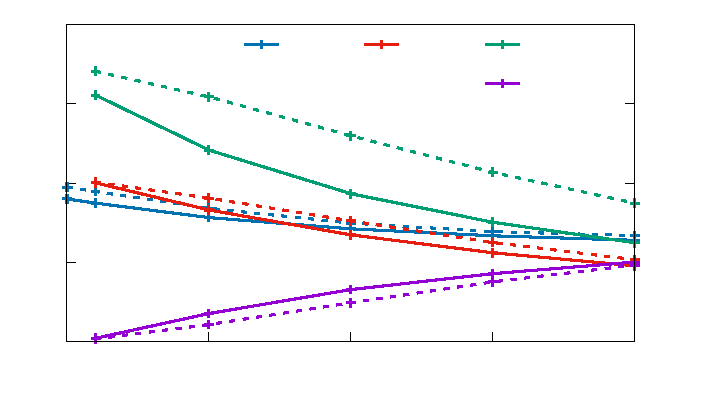
\includegraphics{licl-zif-neighbors}}%
    \gplfronttext
  \end{picture}%
\endgroup

%     \caption{Number of water neighbors in the first solvation shell in the
%     confined liquid (plain lines) and the bulk liquid (dotted lines) as
%     function of the concentration, at the constant pressure of \SI{0}{GPa}.
%     The number of chlorine neighbors for lithium ions is also represented.}
%     \label{fig:licl-zif:neighbors}
% \end{figure}
%
% The first thing we can see here is that, for all species (\ce{Li+}, \ce{Cl-} and
% water), the number of neighboring water molecules --- i.e., the solvation ---
% decreases as the LiCl concentration increases. At \SI{0}{mol/L} and
% \SI{1}{mol/L}, there are more than enough water molecules for each ion (roughly
% 55 water molecule per ion at \SI{1}{mol/L}) so that they can be in their ideal
% solvation state: 4 \ce{H2O} per \ce{Li+}, and 6 \ce{H2O} per \ce{Cl-}. But as
% the concentration increases, there are fewer available water molecules and the
% ions have to accommodate by having less molecule in their first solvation shell.
% At \SI{20}{mol/L}, there are only 2.7 water molecule available for each lithium
% ion; and each cation is thus surrounded by 1.9 water molecule, less than half
% its complete solvation state. The same is true for water/water coordination
% through hydrogen bonds, as the water molecules compete with the ions to surround
% themselves with other water molecules.
%
% \begin{figure}[b]
%     \centering
%     % GNUPLOT: LaTeX picture with Postscript
\begingroup
  \makeatletter
  \providecommand\color[2][]{%
    \GenericError{(gnuplot) \space\space\space\@spaces}{%
      Package color not loaded in conjunction with
      terminal option `colourtext'%
    }{See the gnuplot documentation for explanation.%
    }{Either use 'blacktext' in gnuplot or load the package
      color.sty in LaTeX.}%
    \renewcommand\color[2][]{}%
  }%
  \providecommand\includegraphics[2][]{%
    \GenericError{(gnuplot) \space\space\space\@spaces}{%
      Package graphicx or graphics not loaded%
    }{See the gnuplot documentation for explanation.%
    }{The gnuplot epslatex terminal needs graphicx.sty or graphics.sty.}%
    \renewcommand\includegraphics[2][]{}%
  }%
  \providecommand\rotatebox[2]{#2}%
  \@ifundefined{ifGPcolor}{%
    \newif\ifGPcolor
    \GPcolortrue
  }{}%
  \@ifundefined{ifGPblacktext}{%
    \newif\ifGPblacktext
    \GPblacktextfalse
  }{}%
  % define a \g@addto@macro without @ in the name:
  \let\gplgaddtomacro\g@addto@macro
  % define empty templates for all commands taking text:
  \gdef\gplbacktext{}%
  \gdef\gplfronttext{}%
  \makeatother
  \ifGPblacktext
    % no textcolor at all
    \def\colorrgb#1{}%
    \def\colorgray#1{}%
  \else
    % gray or color?
    \ifGPcolor
      \def\colorrgb#1{\color[rgb]{#1}}%
      \def\colorgray#1{\color[gray]{#1}}%
      \expandafter\def\csname LTw\endcsname{\color{white}}%
      \expandafter\def\csname LTb\endcsname{\color{black}}%
      \expandafter\def\csname LTa\endcsname{\color{black}}%
      \expandafter\def\csname LT0\endcsname{\color[rgb]{1,0,0}}%
      \expandafter\def\csname LT1\endcsname{\color[rgb]{0,1,0}}%
      \expandafter\def\csname LT2\endcsname{\color[rgb]{0,0,1}}%
      \expandafter\def\csname LT3\endcsname{\color[rgb]{1,0,1}}%
      \expandafter\def\csname LT4\endcsname{\color[rgb]{0,1,1}}%
      \expandafter\def\csname LT5\endcsname{\color[rgb]{1,1,0}}%
      \expandafter\def\csname LT6\endcsname{\color[rgb]{0,0,0}}%
      \expandafter\def\csname LT7\endcsname{\color[rgb]{1,0.3,0}}%
      \expandafter\def\csname LT8\endcsname{\color[rgb]{0.5,0.5,0.5}}%
    \else
      % gray
      \def\colorrgb#1{\color{black}}%
      \def\colorgray#1{\color[gray]{#1}}%
      \expandafter\def\csname LTw\endcsname{\color{white}}%
      \expandafter\def\csname LTb\endcsname{\color{black}}%
      \expandafter\def\csname LTa\endcsname{\color{black}}%
      \expandafter\def\csname LT0\endcsname{\color{black}}%
      \expandafter\def\csname LT1\endcsname{\color{black}}%
      \expandafter\def\csname LT2\endcsname{\color{black}}%
      \expandafter\def\csname LT3\endcsname{\color{black}}%
      \expandafter\def\csname LT4\endcsname{\color{black}}%
      \expandafter\def\csname LT5\endcsname{\color{black}}%
      \expandafter\def\csname LT6\endcsname{\color{black}}%
      \expandafter\def\csname LT7\endcsname{\color{black}}%
      \expandafter\def\csname LT8\endcsname{\color{black}}%
    \fi
  \fi
    \setlength{\unitlength}{0.0500bp}%
    \ifx\gptboxheight\undefined%
      \newlength{\gptboxheight}%
      \newlength{\gptboxwidth}%
      \newsavebox{\gptboxtext}%
    \fi%
    \setlength{\fboxrule}{0.5pt}%
    \setlength{\fboxsep}{1pt}%
\begin{picture}(7360.00,7080.00)%
    \gplgaddtomacro\gplbacktext{%
      \csname LTb\endcsname%%
      \put(578,5032){\makebox(0,0)[r]{\strut{}\tiny -0.5}}%
      \csname LTb\endcsname%%
      \put(578,5482){\makebox(0,0)[r]{\strut{}\tiny -0.25}}%
      \csname LTb\endcsname%%
      \put(578,5932){\makebox(0,0)[r]{\strut{}\tiny 0}}%
      \csname LTb\endcsname%%
      \put(578,6382){\makebox(0,0)[r]{\strut{}\tiny 0.25}}%
      \csname LTb\endcsname%%
      \put(578,6832){\makebox(0,0)[r]{\strut{}\tiny 0.5}}%
      \csname LTb\endcsname%%
      \put(646,4908){\makebox(0,0){\strut{}\tiny -0.5}}%
      \csname LTb\endcsname%%
      \put(1096,4908){\makebox(0,0){\strut{}\tiny -0.25}}%
      \csname LTb\endcsname%%
      \put(1546,4908){\makebox(0,0){\strut{}\tiny 0}}%
      \csname LTb\endcsname%%
      \put(1995,4908){\makebox(0,0){\strut{}\tiny 0.25}}%
      \csname LTb\endcsname%%
      \put(2445,4908){\makebox(0,0){\strut{}\tiny 0.5}}%
      \colorrgb{1.00,0.00,0.00}%%
      \put(74,5899){\makebox(0,0)[l]{\strut{}O}}%
      \colorrgb{0.00,0.00,1.00}%%
      \put(74,3681){\makebox(0,0)[l]{\strut{}Li}}%
      \colorrgb{0.00,0.32,0.19}%%
      \put(74,1321){\makebox(0,0)[l]{\strut{}Cl}}%
    }%
    \gplgaddtomacro\gplfronttext{%
      \csname LTb\endcsname%%
      \put(1545,7018){\makebox(0,0){\strut{}1 mol/L}}%
    }%
    \gplgaddtomacro\gplbacktext{%
      \csname LTb\endcsname%%
      \put(2847,5032){\makebox(0,0)[r]{\strut{}\tiny -0.5}}%
      \csname LTb\endcsname%%
      \put(2847,5482){\makebox(0,0)[r]{\strut{}\tiny -0.25}}%
      \csname LTb\endcsname%%
      \put(2847,5932){\makebox(0,0)[r]{\strut{}\tiny 0}}%
      \csname LTb\endcsname%%
      \put(2847,6382){\makebox(0,0)[r]{\strut{}\tiny 0.25}}%
      \csname LTb\endcsname%%
      \put(2847,6832){\makebox(0,0)[r]{\strut{}\tiny 0.5}}%
      \csname LTb\endcsname%%
      \put(2915,4908){\makebox(0,0){\strut{}\tiny -0.5}}%
      \csname LTb\endcsname%%
      \put(3365,4908){\makebox(0,0){\strut{}\tiny -0.25}}%
      \csname LTb\endcsname%%
      \put(3815,4908){\makebox(0,0){\strut{}\tiny 0}}%
      \csname LTb\endcsname%%
      \put(4264,4908){\makebox(0,0){\strut{}\tiny 0.25}}%
      \csname LTb\endcsname%%
      \put(4714,4908){\makebox(0,0){\strut{}\tiny 0.5}}%
      \colorrgb{1.00,0.00,0.00}%%
      \put(74,5899){\makebox(0,0)[l]{\strut{}O}}%
      \colorrgb{0.00,0.00,1.00}%%
      \put(74,3681){\makebox(0,0)[l]{\strut{}Li}}%
      \colorrgb{0.00,0.32,0.19}%%
      \put(74,1321){\makebox(0,0)[l]{\strut{}Cl}}%
    }%
    \gplgaddtomacro\gplfronttext{%
      \csname LTb\endcsname%%
      \put(3814,7018){\makebox(0,0){\strut{}10 mol/L}}%
    }%
    \gplgaddtomacro\gplbacktext{%
      \csname LTb\endcsname%%
      \put(5116,5032){\makebox(0,0)[r]{\strut{}\tiny -0.5}}%
      \csname LTb\endcsname%%
      \put(5116,5482){\makebox(0,0)[r]{\strut{}\tiny -0.25}}%
      \csname LTb\endcsname%%
      \put(5116,5932){\makebox(0,0)[r]{\strut{}\tiny 0}}%
      \csname LTb\endcsname%%
      \put(5116,6382){\makebox(0,0)[r]{\strut{}\tiny 0.25}}%
      \csname LTb\endcsname%%
      \put(5116,6832){\makebox(0,0)[r]{\strut{}\tiny 0.5}}%
      \csname LTb\endcsname%%
      \put(5184,4908){\makebox(0,0){\strut{}\tiny -0.5}}%
      \csname LTb\endcsname%%
      \put(5634,4908){\makebox(0,0){\strut{}\tiny -0.25}}%
      \csname LTb\endcsname%%
      \put(6084,4908){\makebox(0,0){\strut{}\tiny 0}}%
      \csname LTb\endcsname%%
      \put(6533,4908){\makebox(0,0){\strut{}\tiny 0.25}}%
      \csname LTb\endcsname%%
      \put(6983,4908){\makebox(0,0){\strut{}\tiny 0.5}}%
      \colorrgb{1.00,0.00,0.00}%%
      \put(74,5899){\makebox(0,0)[l]{\strut{}O}}%
      \colorrgb{0.00,0.00,1.00}%%
      \put(74,3681){\makebox(0,0)[l]{\strut{}Li}}%
      \colorrgb{0.00,0.32,0.19}%%
      \put(74,1321){\makebox(0,0)[l]{\strut{}Cl}}%
    }%
    \gplgaddtomacro\gplfronttext{%
      \csname LTb\endcsname%%
      \put(6083,7018){\makebox(0,0){\strut{}20 mol/L}}%
    }%
    \gplgaddtomacro\gplbacktext{%
      \csname LTb\endcsname%%
      \put(578,2796){\makebox(0,0)[r]{\strut{}\tiny -0.5}}%
      \csname LTb\endcsname%%
      \put(578,3246){\makebox(0,0)[r]{\strut{}\tiny -0.25}}%
      \csname LTb\endcsname%%
      \put(578,3696){\makebox(0,0)[r]{\strut{}\tiny 0}}%
      \csname LTb\endcsname%%
      \put(578,4146){\makebox(0,0)[r]{\strut{}\tiny 0.25}}%
      \csname LTb\endcsname%%
      \put(578,4596){\makebox(0,0)[r]{\strut{}\tiny 0.5}}%
      \csname LTb\endcsname%%
      \put(646,2672){\makebox(0,0){\strut{}\tiny -0.5}}%
      \csname LTb\endcsname%%
      \put(1096,2672){\makebox(0,0){\strut{}\tiny -0.25}}%
      \csname LTb\endcsname%%
      \put(1546,2672){\makebox(0,0){\strut{}\tiny 0}}%
      \csname LTb\endcsname%%
      \put(1995,2672){\makebox(0,0){\strut{}\tiny 0.25}}%
      \csname LTb\endcsname%%
      \put(2445,2672){\makebox(0,0){\strut{}\tiny 0.5}}%
      \colorrgb{1.00,0.00,0.00}%%
      \put(74,5899){\makebox(0,0)[l]{\strut{}O}}%
      \colorrgb{0.00,0.00,1.00}%%
      \put(74,3681){\makebox(0,0)[l]{\strut{}Li}}%
      \colorrgb{0.00,0.32,0.19}%%
      \put(74,1321){\makebox(0,0)[l]{\strut{}Cl}}%
    }%
    \gplgaddtomacro\gplfronttext{%
    }%
    \gplgaddtomacro\gplbacktext{%
      \csname LTb\endcsname%%
      \put(2847,2796){\makebox(0,0)[r]{\strut{}\tiny -0.5}}%
      \csname LTb\endcsname%%
      \put(2847,3246){\makebox(0,0)[r]{\strut{}\tiny -0.25}}%
      \csname LTb\endcsname%%
      \put(2847,3696){\makebox(0,0)[r]{\strut{}\tiny 0}}%
      \csname LTb\endcsname%%
      \put(2847,4146){\makebox(0,0)[r]{\strut{}\tiny 0.25}}%
      \csname LTb\endcsname%%
      \put(2847,4596){\makebox(0,0)[r]{\strut{}\tiny 0.5}}%
      \csname LTb\endcsname%%
      \put(2915,2672){\makebox(0,0){\strut{}\tiny -0.5}}%
      \csname LTb\endcsname%%
      \put(3365,2672){\makebox(0,0){\strut{}\tiny -0.25}}%
      \csname LTb\endcsname%%
      \put(3815,2672){\makebox(0,0){\strut{}\tiny 0}}%
      \csname LTb\endcsname%%
      \put(4264,2672){\makebox(0,0){\strut{}\tiny 0.25}}%
      \csname LTb\endcsname%%
      \put(4714,2672){\makebox(0,0){\strut{}\tiny 0.5}}%
      \colorrgb{1.00,0.00,0.00}%%
      \put(74,5899){\makebox(0,0)[l]{\strut{}O}}%
      \colorrgb{0.00,0.00,1.00}%%
      \put(74,3681){\makebox(0,0)[l]{\strut{}Li}}%
      \colorrgb{0.00,0.32,0.19}%%
      \put(74,1321){\makebox(0,0)[l]{\strut{}Cl}}%
    }%
    \gplgaddtomacro\gplfronttext{%
    }%
    \gplgaddtomacro\gplbacktext{%
      \csname LTb\endcsname%%
      \put(5116,2796){\makebox(0,0)[r]{\strut{}\tiny -0.5}}%
      \csname LTb\endcsname%%
      \put(5116,3246){\makebox(0,0)[r]{\strut{}\tiny -0.25}}%
      \csname LTb\endcsname%%
      \put(5116,3696){\makebox(0,0)[r]{\strut{}\tiny 0}}%
      \csname LTb\endcsname%%
      \put(5116,4146){\makebox(0,0)[r]{\strut{}\tiny 0.25}}%
      \csname LTb\endcsname%%
      \put(5116,4596){\makebox(0,0)[r]{\strut{}\tiny 0.5}}%
      \csname LTb\endcsname%%
      \put(5184,2672){\makebox(0,0){\strut{}\tiny -0.5}}%
      \csname LTb\endcsname%%
      \put(5634,2672){\makebox(0,0){\strut{}\tiny -0.25}}%
      \csname LTb\endcsname%%
      \put(6084,2672){\makebox(0,0){\strut{}\tiny 0}}%
      \csname LTb\endcsname%%
      \put(6533,2672){\makebox(0,0){\strut{}\tiny 0.25}}%
      \csname LTb\endcsname%%
      \put(6983,2672){\makebox(0,0){\strut{}\tiny 0.5}}%
      \colorrgb{1.00,0.00,0.00}%%
      \put(74,5899){\makebox(0,0)[l]{\strut{}O}}%
      \colorrgb{0.00,0.00,1.00}%%
      \put(74,3681){\makebox(0,0)[l]{\strut{}Li}}%
      \colorrgb{0.00,0.32,0.19}%%
      \put(74,1321){\makebox(0,0)[l]{\strut{}Cl}}%
    }%
    \gplgaddtomacro\gplfronttext{%
    }%
    \gplgaddtomacro\gplbacktext{%
      \csname LTb\endcsname%%
      \put(578,436){\makebox(0,0)[r]{\strut{}\tiny -0.5}}%
      \csname LTb\endcsname%%
      \put(578,886){\makebox(0,0)[r]{\strut{}\tiny -0.25}}%
      \csname LTb\endcsname%%
      \put(578,1336){\makebox(0,0)[r]{\strut{}\tiny 0}}%
      \csname LTb\endcsname%%
      \put(578,1786){\makebox(0,0)[r]{\strut{}\tiny 0.25}}%
      \csname LTb\endcsname%%
      \put(578,2236){\makebox(0,0)[r]{\strut{}\tiny 0.5}}%
      \csname LTb\endcsname%%
      \put(646,312){\makebox(0,0){\strut{}\tiny -0.5}}%
      \csname LTb\endcsname%%
      \put(1096,312){\makebox(0,0){\strut{}\tiny -0.25}}%
      \csname LTb\endcsname%%
      \put(1546,312){\makebox(0,0){\strut{}\tiny 0}}%
      \csname LTb\endcsname%%
      \put(1995,312){\makebox(0,0){\strut{}\tiny 0.25}}%
      \csname LTb\endcsname%%
      \put(2445,312){\makebox(0,0){\strut{}\tiny 0.5}}%
      \colorrgb{1.00,0.00,0.00}%%
      \put(74,5899){\makebox(0,0)[l]{\strut{}O}}%
      \colorrgb{0.00,0.00,1.00}%%
      \put(74,3681){\makebox(0,0)[l]{\strut{}Li}}%
      \colorrgb{0.00,0.32,0.19}%%
      \put(74,1321){\makebox(0,0)[l]{\strut{}Cl}}%
    }%
    \gplgaddtomacro\gplfronttext{%
    }%
    \gplgaddtomacro\gplbacktext{%
      \csname LTb\endcsname%%
      \put(2847,436){\makebox(0,0)[r]{\strut{}\tiny -0.5}}%
      \csname LTb\endcsname%%
      \put(2847,886){\makebox(0,0)[r]{\strut{}\tiny -0.25}}%
      \csname LTb\endcsname%%
      \put(2847,1336){\makebox(0,0)[r]{\strut{}\tiny 0}}%
      \csname LTb\endcsname%%
      \put(2847,1786){\makebox(0,0)[r]{\strut{}\tiny 0.25}}%
      \csname LTb\endcsname%%
      \put(2847,2236){\makebox(0,0)[r]{\strut{}\tiny 0.5}}%
      \csname LTb\endcsname%%
      \put(2915,312){\makebox(0,0){\strut{}\tiny -0.5}}%
      \csname LTb\endcsname%%
      \put(3365,312){\makebox(0,0){\strut{}\tiny -0.25}}%
      \csname LTb\endcsname%%
      \put(3815,312){\makebox(0,0){\strut{}\tiny 0}}%
      \csname LTb\endcsname%%
      \put(4264,312){\makebox(0,0){\strut{}\tiny 0.25}}%
      \csname LTb\endcsname%%
      \put(4714,312){\makebox(0,0){\strut{}\tiny 0.5}}%
      \colorrgb{1.00,0.00,0.00}%%
      \put(74,5899){\makebox(0,0)[l]{\strut{}O}}%
      \colorrgb{0.00,0.00,1.00}%%
      \put(74,3681){\makebox(0,0)[l]{\strut{}Li}}%
      \colorrgb{0.00,0.32,0.19}%%
      \put(74,1321){\makebox(0,0)[l]{\strut{}Cl}}%
    }%
    \gplgaddtomacro\gplfronttext{%
    }%
    \gplgaddtomacro\gplbacktext{%
      \csname LTb\endcsname%%
      \put(5116,436){\makebox(0,0)[r]{\strut{}\tiny -0.5}}%
      \csname LTb\endcsname%%
      \put(5116,886){\makebox(0,0)[r]{\strut{}\tiny -0.25}}%
      \csname LTb\endcsname%%
      \put(5116,1336){\makebox(0,0)[r]{\strut{}\tiny 0}}%
      \csname LTb\endcsname%%
      \put(5116,1786){\makebox(0,0)[r]{\strut{}\tiny 0.25}}%
      \csname LTb\endcsname%%
      \put(5116,2236){\makebox(0,0)[r]{\strut{}\tiny 0.5}}%
      \csname LTb\endcsname%%
      \put(5184,312){\makebox(0,0){\strut{}\tiny -0.5}}%
      \csname LTb\endcsname%%
      \put(5634,312){\makebox(0,0){\strut{}\tiny -0.25}}%
      \csname LTb\endcsname%%
      \put(6084,312){\makebox(0,0){\strut{}\tiny 0}}%
      \csname LTb\endcsname%%
      \put(6533,312){\makebox(0,0){\strut{}\tiny 0.25}}%
      \csname LTb\endcsname%%
      \put(6983,312){\makebox(0,0){\strut{}\tiny 0.5}}%
      \colorrgb{1.00,0.00,0.00}%%
      \put(74,5899){\makebox(0,0)[l]{\strut{}O}}%
      \colorrgb{0.00,0.00,1.00}%%
      \put(74,3681){\makebox(0,0)[l]{\strut{}Li}}%
      \colorrgb{0.00,0.32,0.19}%%
      \put(74,1321){\makebox(0,0)[l]{\strut{}Cl}}%
    }%
    \gplgaddtomacro\gplfronttext{%
    }%
    \gplbacktext
    \put(0,0){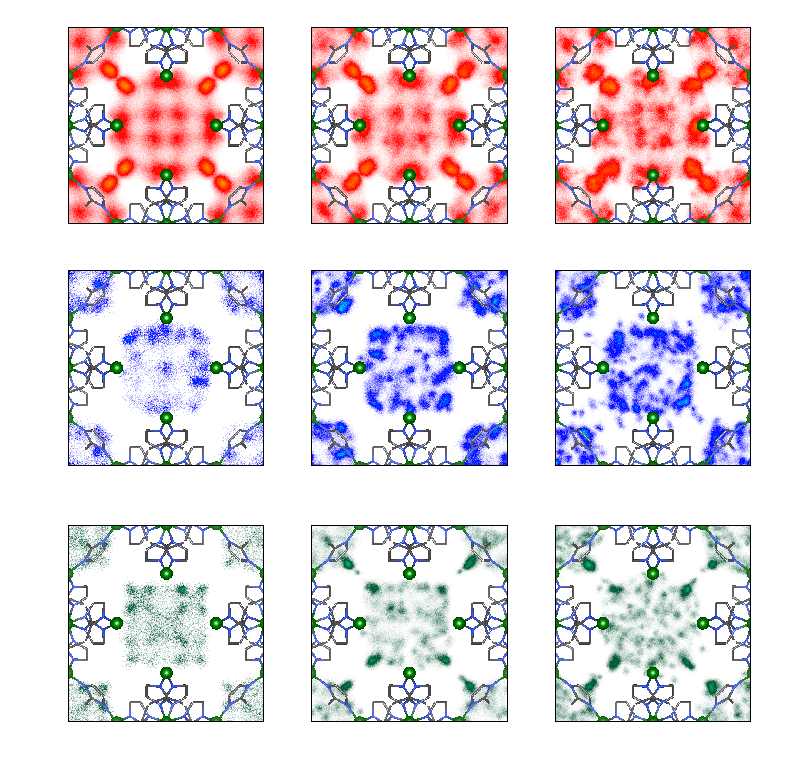
\includegraphics{licl-zif-density}}%
    \gplfronttext
  \end{picture}%
\endgroup

%     \caption{Two-dimensional density profile of oxygen (top), lithium (middle) and
%     chlorine (bottom) atoms in LiCl electrolyte confined in \ZIF8 at \SI{0}{GPa}
%     as a function of LiCl concentration (left to right). The atoms from the
%     \ZIF8 framework are superimposed, with some linkers omitted for clarity
%     between the four central zinc atoms.}
%     \label{fig:licl-zif:density}
% \end{figure}
%
% In the bulk liquid, the loss of neighbors is linear with the concentration, as
% all the molecules in the system are able to adapt to find the state of largest
% possible solvation. In the confined liquid however, the molecules are
% geometrically constrained by the presence of the \ZIF8 framework, which
% manifests as an excluded volume, and thus are not able to adapt as well to the
% increase in LiCl concentration, making the number of neighbors drop faster. We
% also note a slight increase in the number of chlorine neighbors of lithium ions
% at intermediate concentration, compared to the bulk: the effect of confinement,
% by diminishing the solvation of the ions, favors the occurrence of anion--cation
% pairs. The number of lithium neighbors for chlorine ions is the same as the
% number of chlorine neighbors for lithium ions.
%
% Going from bulk liquid to confined liquid also changes the number of neighbors
% for water and Cl ions, even at \SI{1}{mol/L}. In addition to preventing a full
% reorganization of the water molecules when the concentration increases, the
% presence of the framework also affects the structure of the solvation shells.
% Molecules close to the framework can only have neighbors from the liquid on one
% side --- this is an excluded volume effect. However, the framework also has an
% effect at longer range, the available space in the pores dictating the
% arrangement of molecules. Instead of being widely distributed, the molecules are
% restricted to specific preferential locations, due to host--guest interactions.
% This effect is particularly visible on figure~\ref{fig:licl-zif:density}, and is
% stronger on Cl/water pairs than water/water or Li/water, as the Cl has a larger
% radius and binds to the hydrogen atoms in water, making its solvation sphere
% both bigger and "softer".
%
% \begin{figure}[p]
%     \centering
%     % GNUPLOT: LaTeX picture with Postscript
\begingroup
  \makeatletter
  \providecommand\color[2][]{%
    \GenericError{(gnuplot) \space\space\space\@spaces}{%
      Package color not loaded in conjunction with
      terminal option `colourtext'%
    }{See the gnuplot documentation for explanation.%
    }{Either use 'blacktext' in gnuplot or load the package
      color.sty in LaTeX.}%
    \renewcommand\color[2][]{}%
  }%
  \providecommand\includegraphics[2][]{%
    \GenericError{(gnuplot) \space\space\space\@spaces}{%
      Package graphicx or graphics not loaded%
    }{See the gnuplot documentation for explanation.%
    }{The gnuplot epslatex terminal needs graphicx.sty or graphics.sty.}%
    \renewcommand\includegraphics[2][]{}%
  }%
  \providecommand\rotatebox[2]{#2}%
  \@ifundefined{ifGPcolor}{%
    \newif\ifGPcolor
    \GPcolortrue
  }{}%
  \@ifundefined{ifGPblacktext}{%
    \newif\ifGPblacktext
    \GPblacktextfalse
  }{}%
  % define a \g@addto@macro without @ in the name:
  \let\gplgaddtomacro\g@addto@macro
  % define empty templates for all commands taking text:
  \gdef\gplbacktext{}%
  \gdef\gplfronttext{}%
  \makeatother
  \ifGPblacktext
    % no textcolor at all
    \def\colorrgb#1{}%
    \def\colorgray#1{}%
  \else
    % gray or color?
    \ifGPcolor
      \def\colorrgb#1{\color[rgb]{#1}}%
      \def\colorgray#1{\color[gray]{#1}}%
      \expandafter\def\csname LTw\endcsname{\color{white}}%
      \expandafter\def\csname LTb\endcsname{\color{black}}%
      \expandafter\def\csname LTa\endcsname{\color{black}}%
      \expandafter\def\csname LT0\endcsname{\color[rgb]{1,0,0}}%
      \expandafter\def\csname LT1\endcsname{\color[rgb]{0,1,0}}%
      \expandafter\def\csname LT2\endcsname{\color[rgb]{0,0,1}}%
      \expandafter\def\csname LT3\endcsname{\color[rgb]{1,0,1}}%
      \expandafter\def\csname LT4\endcsname{\color[rgb]{0,1,1}}%
      \expandafter\def\csname LT5\endcsname{\color[rgb]{1,1,0}}%
      \expandafter\def\csname LT6\endcsname{\color[rgb]{0,0,0}}%
      \expandafter\def\csname LT7\endcsname{\color[rgb]{1,0.3,0}}%
      \expandafter\def\csname LT8\endcsname{\color[rgb]{0.5,0.5,0.5}}%
    \else
      % gray
      \def\colorrgb#1{\color{black}}%
      \def\colorgray#1{\color[gray]{#1}}%
      \expandafter\def\csname LTw\endcsname{\color{white}}%
      \expandafter\def\csname LTb\endcsname{\color{black}}%
      \expandafter\def\csname LTa\endcsname{\color{black}}%
      \expandafter\def\csname LT0\endcsname{\color{black}}%
      \expandafter\def\csname LT1\endcsname{\color{black}}%
      \expandafter\def\csname LT2\endcsname{\color{black}}%
      \expandafter\def\csname LT3\endcsname{\color{black}}%
      \expandafter\def\csname LT4\endcsname{\color{black}}%
      \expandafter\def\csname LT5\endcsname{\color{black}}%
      \expandafter\def\csname LT6\endcsname{\color{black}}%
      \expandafter\def\csname LT7\endcsname{\color{black}}%
      \expandafter\def\csname LT8\endcsname{\color{black}}%
    \fi
  \fi
    \setlength{\unitlength}{0.0500bp}%
    \ifx\gptboxheight\undefined%
      \newlength{\gptboxheight}%
      \newlength{\gptboxwidth}%
      \newsavebox{\gptboxtext}%
    \fi%
    \setlength{\fboxrule}{0.5pt}%
    \setlength{\fboxsep}{1pt}%
\begin{picture}(6500.00,12000.00)%
    \gplgaddtomacro\gplbacktext{%
    }%
    \gplgaddtomacro\gplfronttext{%
      \csname LTb\endcsname%%
      \put(1126,11693){\makebox(0,0){\strut{}\small 0 mol/L}}%
    }%
    \gplgaddtomacro\gplbacktext{%
    }%
    \gplgaddtomacro\gplfronttext{%
      \csname LTb\endcsname%%
      \put(3249,11693){\makebox(0,0){\strut{}\small 1 mol/L}}%
    }%
    \gplgaddtomacro\gplbacktext{%
    }%
    \gplgaddtomacro\gplfronttext{%
      \csname LTb\endcsname%%
      \put(5372,11693){\makebox(0,0){\strut{}\small 5 mol/L}}%
    }%
    \gplgaddtomacro\gplbacktext{%
    }%
    \gplgaddtomacro\gplfronttext{%
      \csname LTb\endcsname%%
      \put(1126,9733){\makebox(0,0){\strut{}\small 10 mol/L}}%
    }%
    \gplgaddtomacro\gplbacktext{%
    }%
    \gplgaddtomacro\gplfronttext{%
      \csname LTb\endcsname%%
      \put(3249,9733){\makebox(0,0){\strut{}\small 15 mol/L}}%
    }%
    \gplgaddtomacro\gplbacktext{%
    }%
    \gplgaddtomacro\gplfronttext{%
      \csname LTb\endcsname%%
      \put(5372,9733){\makebox(0,0){\strut{}\small 20 mol/L}}%
    }%
    \gplgaddtomacro\gplbacktext{%
    }%
    \gplgaddtomacro\gplfronttext{%
      \csname LTb\endcsname%%
      \put(3249,7773){\makebox(0,0){\strut{}\small 1 mol/L}}%
    }%
    \gplgaddtomacro\gplbacktext{%
    }%
    \gplgaddtomacro\gplfronttext{%
      \csname LTb\endcsname%%
      \put(5372,7773){\makebox(0,0){\strut{}\small 5 mol/L}}%
    }%
    \gplgaddtomacro\gplbacktext{%
    }%
    \gplgaddtomacro\gplfronttext{%
      \csname LTb\endcsname%%
      \put(1126,5813){\makebox(0,0){\strut{}\small 10 mol/L}}%
    }%
    \gplgaddtomacro\gplbacktext{%
    }%
    \gplgaddtomacro\gplfronttext{%
      \csname LTb\endcsname%%
      \put(3249,5813){\makebox(0,0){\strut{}\small 15 mol/L}}%
    }%
    \gplgaddtomacro\gplbacktext{%
    }%
    \gplgaddtomacro\gplfronttext{%
      \csname LTb\endcsname%%
      \put(5372,5813){\makebox(0,0){\strut{}\small 20 mol/L}}%
    }%
    \gplgaddtomacro\gplbacktext{%
    }%
    \gplgaddtomacro\gplfronttext{%
      \csname LTb\endcsname%%
      \put(3249,3853){\makebox(0,0){\strut{}\small 1 mol/L}}%
    }%
    \gplgaddtomacro\gplbacktext{%
    }%
    \gplgaddtomacro\gplfronttext{%
      \csname LTb\endcsname%%
      \put(5372,3853){\makebox(0,0){\strut{}\small 5 mol/L}}%
    }%
    \gplgaddtomacro\gplbacktext{%
    }%
    \gplgaddtomacro\gplfronttext{%
      \csname LTb\endcsname%%
      \put(1126,1893){\makebox(0,0){\strut{}\small 10 mol/L}}%
    }%
    \gplgaddtomacro\gplbacktext{%
    }%
    \gplgaddtomacro\gplfronttext{%
      \csname LTb\endcsname%%
      \put(3249,1893){\makebox(0,0){\strut{}\small 15 mol/L}}%
    }%
    \gplgaddtomacro\gplbacktext{%
    }%
    \gplgaddtomacro\gplfronttext{%
      \csname LTb\endcsname%%
      \put(5372,1893){\makebox(0,0){\strut{}\small 20 mol/L}}%
    }%
    \gplbacktext
    \put(0,0){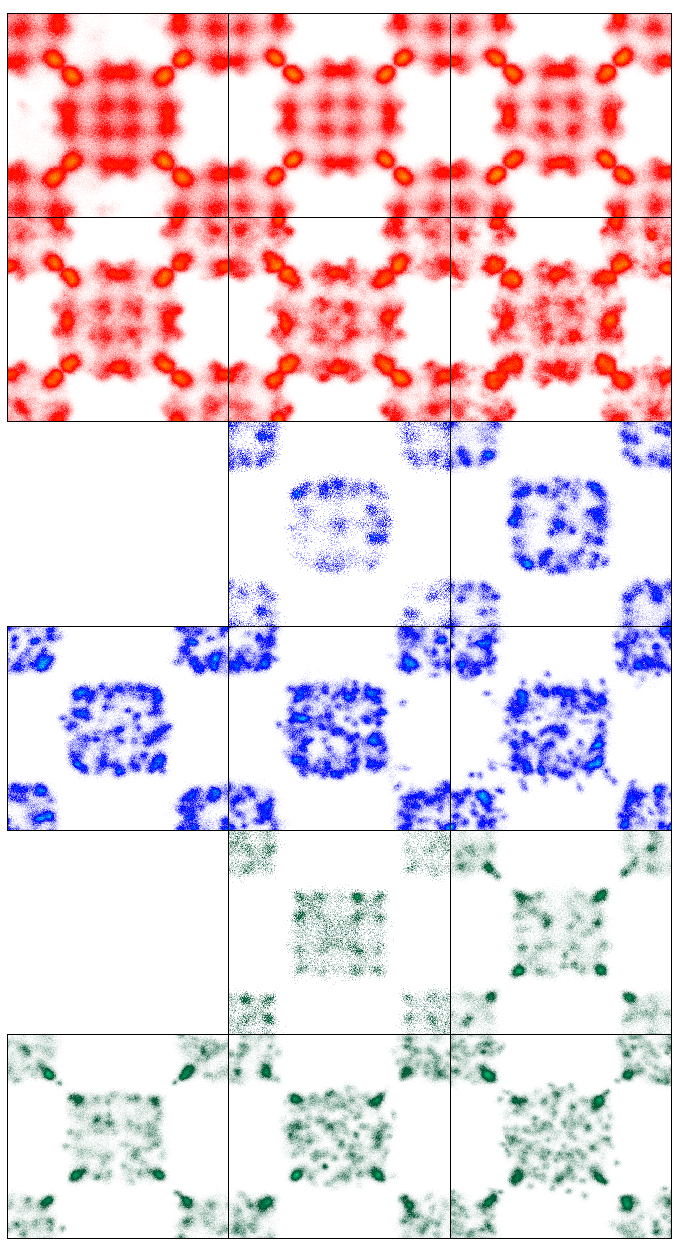
\includegraphics{licl-zif-density-all}}%
    \gplfronttext
  \end{picture}%
\endgroup

%     \caption{2 dimensional density profile of oxygen (red), lithium (blue) and
%     chlorine (green) atoms in LiCl electrolyte confined in \ZIF8 at \SI{0}{GPa}
%     as a function of LiCl concentration. Every graph is presented in fractional
%     coordinates between -0.5 and 0.5.}
%     \label{fig:licl-zif:density:all}
% \end{figure}
%
%
% I also computed in figures~\ref{fig:licl-zif:density}
% and~\ref{fig:licl-zif:density:all} the density profile of atoms in the confined
% liquid, represented in the $xy$ plane, averaged over $z$ and the
% $3\times3\times3$ super-cell. To account for cell deformation during the $NPT$
% simulations, I used fractional coordinates to represent the positions of atoms.
%
% Here we clearly see the long distance structuration of water inside the \ZIF8
% pores. At low concentration (\SI{1}{mol/L}), the water molecules occupy very
% well-defined sites, in particular inside the windows between two neighboring
% cages. As the concentration increases, this organization is perturbed by the
% ions inserted in the water molecules' network --- however this effect is
% relatively small, and the water distribution is not greatly affected. The same
% can be observed in the distribution of chlorine ions, with a well defined, high
% symmetry distribution at low concentration, but as the concentration increases
% the distribution of ions becomes more and more distributed over the whole pore
% space. Concerning lithium ions, they present a looser arrangement inside the
% pores, and are distributed relatively evenly, yet present a preferential
% occupation next to the water molecules in the 6-member windows (in the diagonal
% in figure~\ref{fig:licl-zif:density}).
%
% These results can be explained by both the difference in kinetic
% radius\cite{Marcus1988} for water molecules (\SI{2.65}{\AA}), chlorine
% ions (\SI{3.2}{\AA}) and lithium ions (\SI{2.1}{\AA}), as well as
% the strong attraction between water oxygen atoms and lithium. The difference in
% size allows lithium ions to fit in smaller spaces, and an even distribution of
% ions will increase the total entropy of the system. At the same time, chlorine
% ions and water molecules are more polarizable than lithium, and as such will
% have stronger interactions with the aromatic linkers, making it preferable for
% them to take the highly organized arrangement we observe.
%
% \FloatBarrier
% \subsection{Dynamics under confinement}
%
% I used two different indicators to quantify the dynamics of water molecules
% confined in \ZIF8 and the impact of LiCl concentration and pressure on this
% dynamic. The first one is based on the lifetime of hydrogen bonds between water
% molecules. Following \citeauthor{Luzar1996}\cite{Luzar1996}, I characterize the
% presence of a hydrogen bond between two water molecules as two oxygen atoms
% separated by less than \SI{3.5}{\AA}, with an oxygen--oxygen--hydrogen
% ($\widehat{\text{OOH}}$) angle less than 30\textdegree. I then computed the
% time autocorrelation function of the hydrogen bond existence functions $H(t)$
% --- set to 1 if the bond exists at time $t$, 0 if is does not exists --- as:
% \[C_{\text{hbonds}}(t) = \left\langle H(t_0) \cdot H(t_0 + t) \right\rangle_{t_0} \]
% The decay of this autocorrelation function, presented in
% figure~\ref{fig:licl-zif:hbonds}, is characteristic of the dynamics of the
% hydrogen bond network and the lifetime of individual hydrogen bonds.
%
% \begin{figure}[ht]
%     \centering
%     % GNUPLOT: LaTeX picture with Postscript
\begingroup
  \makeatletter
  \providecommand\color[2][]{%
    \GenericError{(gnuplot) \space\space\space\@spaces}{%
      Package color not loaded in conjunction with
      terminal option `colourtext'%
    }{See the gnuplot documentation for explanation.%
    }{Either use 'blacktext' in gnuplot or load the package
      color.sty in LaTeX.}%
    \renewcommand\color[2][]{}%
  }%
  \providecommand\includegraphics[2][]{%
    \GenericError{(gnuplot) \space\space\space\@spaces}{%
      Package graphicx or graphics not loaded%
    }{See the gnuplot documentation for explanation.%
    }{The gnuplot epslatex terminal needs graphicx.sty or graphics.sty.}%
    \renewcommand\includegraphics[2][]{}%
  }%
  \providecommand\rotatebox[2]{#2}%
  \@ifundefined{ifGPcolor}{%
    \newif\ifGPcolor
    \GPcolortrue
  }{}%
  \@ifundefined{ifGPblacktext}{%
    \newif\ifGPblacktext
    \GPblacktextfalse
  }{}%
  % define a \g@addto@macro without @ in the name:
  \let\gplgaddtomacro\g@addto@macro
  % define empty templates for all commands taking text:
  \gdef\gplbacktext{}%
  \gdef\gplfronttext{}%
  \makeatother
  \ifGPblacktext
    % no textcolor at all
    \def\colorrgb#1{}%
    \def\colorgray#1{}%
  \else
    % gray or color?
    \ifGPcolor
      \def\colorrgb#1{\color[rgb]{#1}}%
      \def\colorgray#1{\color[gray]{#1}}%
      \expandafter\def\csname LTw\endcsname{\color{white}}%
      \expandafter\def\csname LTb\endcsname{\color{black}}%
      \expandafter\def\csname LTa\endcsname{\color{black}}%
      \expandafter\def\csname LT0\endcsname{\color[rgb]{1,0,0}}%
      \expandafter\def\csname LT1\endcsname{\color[rgb]{0,1,0}}%
      \expandafter\def\csname LT2\endcsname{\color[rgb]{0,0,1}}%
      \expandafter\def\csname LT3\endcsname{\color[rgb]{1,0,1}}%
      \expandafter\def\csname LT4\endcsname{\color[rgb]{0,1,1}}%
      \expandafter\def\csname LT5\endcsname{\color[rgb]{1,1,0}}%
      \expandafter\def\csname LT6\endcsname{\color[rgb]{0,0,0}}%
      \expandafter\def\csname LT7\endcsname{\color[rgb]{1,0.3,0}}%
      \expandafter\def\csname LT8\endcsname{\color[rgb]{0.5,0.5,0.5}}%
    \else
      % gray
      \def\colorrgb#1{\color{black}}%
      \def\colorgray#1{\color[gray]{#1}}%
      \expandafter\def\csname LTw\endcsname{\color{white}}%
      \expandafter\def\csname LTb\endcsname{\color{black}}%
      \expandafter\def\csname LTa\endcsname{\color{black}}%
      \expandafter\def\csname LT0\endcsname{\color{black}}%
      \expandafter\def\csname LT1\endcsname{\color{black}}%
      \expandafter\def\csname LT2\endcsname{\color{black}}%
      \expandafter\def\csname LT3\endcsname{\color{black}}%
      \expandafter\def\csname LT4\endcsname{\color{black}}%
      \expandafter\def\csname LT5\endcsname{\color{black}}%
      \expandafter\def\csname LT6\endcsname{\color{black}}%
      \expandafter\def\csname LT7\endcsname{\color{black}}%
      \expandafter\def\csname LT8\endcsname{\color{black}}%
    \fi
  \fi
    \setlength{\unitlength}{0.0500bp}%
    \ifx\gptboxheight\undefined%
      \newlength{\gptboxheight}%
      \newlength{\gptboxwidth}%
      \newsavebox{\gptboxtext}%
    \fi%
    \setlength{\fboxrule}{0.5pt}%
    \setlength{\fboxsep}{1pt}%
\begin{picture}(5660.00,5660.00)%
    \gplgaddtomacro\gplbacktext{%
      \csname LTb\endcsname%%
      \put(752,3264){\makebox(0,0)[r]{\strut{}$0$}}%
      \csname LTb\endcsname%%
      \put(752,3700){\makebox(0,0)[r]{\strut{}$0.2$}}%
      \csname LTb\endcsname%%
      \put(752,4135){\makebox(0,0)[r]{\strut{}$0.4$}}%
      \csname LTb\endcsname%%
      \put(752,4571){\makebox(0,0)[r]{\strut{}$0.6$}}%
      \csname LTb\endcsname%%
      \put(752,5006){\makebox(0,0)[r]{\strut{}$0.8$}}%
      \csname LTb\endcsname%%
      \put(752,5442){\makebox(0,0)[r]{\strut{}$1$}}%
      \csname LTb\endcsname%%
      \put(871,3047){\makebox(0,0){\strut{}$0$}}%
      \csname LTb\endcsname%%
      \put(1979,3047){\makebox(0,0){\strut{}$5$}}%
      \csname LTb\endcsname%%
      \put(3087,3047){\makebox(0,0){\strut{}$10$}}%
      \csname LTb\endcsname%%
      \put(4194,3047){\makebox(0,0){\strut{}$15$}}%
      \csname LTb\endcsname%%
      \put(5302,3047){\makebox(0,0){\strut{}$20$}}%
    }%
    \gplgaddtomacro\gplfronttext{%
      \csname LTb\endcsname%%
      \put(178,4353){\rotatebox{-270}{\makebox(0,0){\strut{}auto correlation}}}%
      \csname LTb\endcsname%%
      \put(2631,5247){\makebox(0,0)[r]{\strut{}0 mol/L}}%
      \csname LTb\endcsname%%
      \put(2631,5030){\makebox(0,0)[r]{\strut{}1 mol/L}}%
      \csname LTb\endcsname%%
      \put(2631,4813){\makebox(0,0)[r]{\strut{}5 mol/L}}%
      \csname LTb\endcsname%%
      \put(4383,5247){\makebox(0,0)[r]{\strut{}10 mol/L}}%
      \csname LTb\endcsname%%
      \put(4383,5030){\makebox(0,0)[r]{\strut{}15 mol/L}}%
      \csname LTb\endcsname%%
      \put(4383,4813){\makebox(0,0)[r]{\strut{}20 mol/L}}%
    }%
    \gplgaddtomacro\gplbacktext{%
      \csname LTb\endcsname%%
      \put(752,694){\makebox(0,0)[r]{\strut{}$0$}}%
      \csname LTb\endcsname%%
      \put(752,1078){\makebox(0,0)[r]{\strut{}$0.2$}}%
      \csname LTb\endcsname%%
      \put(752,1462){\makebox(0,0)[r]{\strut{}$0.4$}}%
      \csname LTb\endcsname%%
      \put(752,1845){\makebox(0,0)[r]{\strut{}$0.6$}}%
      \csname LTb\endcsname%%
      \put(752,2229){\makebox(0,0)[r]{\strut{}$0.8$}}%
      \csname LTb\endcsname%%
      \put(752,2613){\makebox(0,0)[r]{\strut{}$1$}}%
      \csname LTb\endcsname%%
      \put(871,477){\makebox(0,0){\strut{}$0$}}%
      \csname LTb\endcsname%%
      \put(1979,477){\makebox(0,0){\strut{}$5$}}%
      \csname LTb\endcsname%%
      \put(3087,477){\makebox(0,0){\strut{}$10$}}%
      \csname LTb\endcsname%%
      \put(4194,477){\makebox(0,0){\strut{}$15$}}%
      \csname LTb\endcsname%%
      \put(5302,477){\makebox(0,0){\strut{}$20$}}%
    }%
    \gplgaddtomacro\gplfronttext{%
      \csname LTb\endcsname%%
      \put(178,1653){\rotatebox{-270}{\makebox(0,0){\strut{}auto correlation}}}%
      \csname LTb\endcsname%%
      \put(3086,152){\makebox(0,0){\strut{}time (ps)}}%
    }%
    \gplbacktext
    \put(0,0){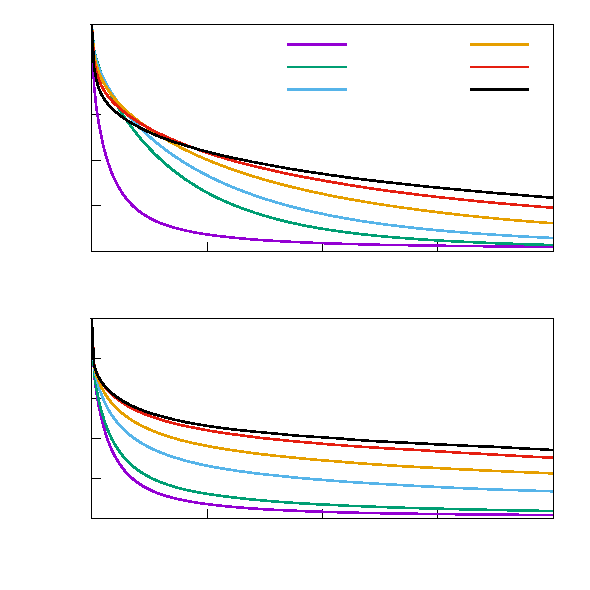
\includegraphics{licl-zif-hbonds}}%
    \gplfronttext
  \end{picture}%
\endgroup

%     \caption{Hydrogen bonds existence autocorrelation in bulk (left) and
%     confined (right) electrolyte as function of LiCl concentration.}
%     \label{fig:licl-zif:hbonds}
% \end{figure}
%
% I then fitted all the autocorrelation functions with bi-exponential functions:
% \[ f(t) = A_1 e^{-t / \tau_1} + A_2 e^{-t / \tau_2}, \]
% where $\tau_1$ and $\tau_2$ are the two time scales of decay, and $A_1$ and
% $A_2$ are their relative weights. The resulting fit parameters are presented in
% table~\ref{table:licl-zif:hbonds} and figure~\ref{fig:licl-zif:hbonds:fit:pressure}.
%
% \begin{table}[b]
%     \caption{Fit coefficients for the hydrogen bonds autocorrelation decay at \SI{0}{GPa}.}
%     \label{table:licl-zif:hbonds}
%     \centering
%     \begin{tabular}{c c c c c c c c c c}
%         \toprule
%         \multicolumn{1}{c}{~} & \multicolumn{4}{c}{Bulk}                          &~& \multicolumn{4}{c}{Confined} \\
%         \multicolumn{1}{c}{~} & $\tau_1$ (ps) & $\tau_2$ (ps) & $A_1$   & $A_2$   &~& $\tau_1$ (ps) & $\tau_2$ (ps) & $A_1$   & $A_2$   \\
%         \midrule
%         \SI{0}{mol/L}         &    3.27       &    9.84       & 69.7 \% & 15.4 \% &~&  1.41         &  11.3         & 45.2 \% & 8.94 \% \\
%         \SI{1}{mol/L}         &    3.36       &    10.1       & 67.0 \% & 17.3 \% &~&  1.56         &  13.8         & 42.3 \% & 15.0 \% \\
%         \SI{5}{mol/L}         &    3.70       &    11.1       & 48.8 \% & 32.4 \% &~&  2.05         &  26.8         & 35.4 \% & 28.0 \% \\
%         \SI{10}{mol/L}        &    3.31       &    14.6       & 30.3 \% & 47.2 \% &~&  2.31         &  38.7         & 29.1 \% & 37.4 \% \\
%         \SI{15}{mol/L}        &    3.28       &    21.5       & 25.5 \% & 47.6 \% &~&  2.37         &  49.3         & 23.8 \% & 45.7 \% \\
%         \SI{20}{mol/L}        &    2.87       &    27.7       & 20.9 \% & 47.9 \% &~&  2.36         &  61.9         & 22.0 \% & 47.5 \% \\
%         \bottomrule
%     \end{tabular}
% \end{table}
%
% \begin{figure}[ht]
%     \centering
%     % GNUPLOT: LaTeX picture with Postscript
\begingroup
  \makeatletter
  \providecommand\color[2][]{%
    \GenericError{(gnuplot) \space\space\space\@spaces}{%
      Package color not loaded in conjunction with
      terminal option `colourtext'%
    }{See the gnuplot documentation for explanation.%
    }{Either use 'blacktext' in gnuplot or load the package
      color.sty in LaTeX.}%
    \renewcommand\color[2][]{}%
  }%
  \providecommand\includegraphics[2][]{%
    \GenericError{(gnuplot) \space\space\space\@spaces}{%
      Package graphicx or graphics not loaded%
    }{See the gnuplot documentation for explanation.%
    }{The gnuplot epslatex terminal needs graphicx.sty or graphics.sty.}%
    \renewcommand\includegraphics[2][]{}%
  }%
  \providecommand\rotatebox[2]{#2}%
  \@ifundefined{ifGPcolor}{%
    \newif\ifGPcolor
    \GPcolortrue
  }{}%
  \@ifundefined{ifGPblacktext}{%
    \newif\ifGPblacktext
    \GPblacktextfalse
  }{}%
  % define a \g@addto@macro without @ in the name:
  \let\gplgaddtomacro\g@addto@macro
  % define empty templates for all commands taking text:
  \gdef\gplbacktext{}%
  \gdef\gplfronttext{}%
  \makeatother
  \ifGPblacktext
    % no textcolor at all
    \def\colorrgb#1{}%
    \def\colorgray#1{}%
  \else
    % gray or color?
    \ifGPcolor
      \def\colorrgb#1{\color[rgb]{#1}}%
      \def\colorgray#1{\color[gray]{#1}}%
      \expandafter\def\csname LTw\endcsname{\color{white}}%
      \expandafter\def\csname LTb\endcsname{\color{black}}%
      \expandafter\def\csname LTa\endcsname{\color{black}}%
      \expandafter\def\csname LT0\endcsname{\color[rgb]{1,0,0}}%
      \expandafter\def\csname LT1\endcsname{\color[rgb]{0,1,0}}%
      \expandafter\def\csname LT2\endcsname{\color[rgb]{0,0,1}}%
      \expandafter\def\csname LT3\endcsname{\color[rgb]{1,0,1}}%
      \expandafter\def\csname LT4\endcsname{\color[rgb]{0,1,1}}%
      \expandafter\def\csname LT5\endcsname{\color[rgb]{1,1,0}}%
      \expandafter\def\csname LT6\endcsname{\color[rgb]{0,0,0}}%
      \expandafter\def\csname LT7\endcsname{\color[rgb]{1,0.3,0}}%
      \expandafter\def\csname LT8\endcsname{\color[rgb]{0.5,0.5,0.5}}%
    \else
      % gray
      \def\colorrgb#1{\color{black}}%
      \def\colorgray#1{\color[gray]{#1}}%
      \expandafter\def\csname LTw\endcsname{\color{white}}%
      \expandafter\def\csname LTb\endcsname{\color{black}}%
      \expandafter\def\csname LTa\endcsname{\color{black}}%
      \expandafter\def\csname LT0\endcsname{\color{black}}%
      \expandafter\def\csname LT1\endcsname{\color{black}}%
      \expandafter\def\csname LT2\endcsname{\color{black}}%
      \expandafter\def\csname LT3\endcsname{\color{black}}%
      \expandafter\def\csname LT4\endcsname{\color{black}}%
      \expandafter\def\csname LT5\endcsname{\color{black}}%
      \expandafter\def\csname LT6\endcsname{\color{black}}%
      \expandafter\def\csname LT7\endcsname{\color{black}}%
      \expandafter\def\csname LT8\endcsname{\color{black}}%
    \fi
  \fi
    \setlength{\unitlength}{0.0500bp}%
    \ifx\gptboxheight\undefined%
      \newlength{\gptboxheight}%
      \newlength{\gptboxwidth}%
      \newsavebox{\gptboxtext}%
    \fi%
    \setlength{\fboxrule}{0.5pt}%
    \setlength{\fboxsep}{1pt}%
\begin{picture}(7580.00,5100.00)%
    \gplgaddtomacro\gplbacktext{%
      \csname LTb\endcsname%%
      \put(408,2667){\makebox(0,0)[r]{\strut{}$0$}}%
      \csname LTb\endcsname%%
      \put(408,3037){\makebox(0,0)[r]{\strut{}$1$}}%
      \csname LTb\endcsname%%
      \put(408,3408){\makebox(0,0)[r]{\strut{}$2$}}%
      \csname LTb\endcsname%%
      \put(408,3778){\makebox(0,0)[r]{\strut{}$3$}}%
      \csname LTb\endcsname%%
      \put(408,4148){\makebox(0,0)[r]{\strut{}$4$}}%
      \csname LTb\endcsname%%
      \put(510,2481){\makebox(0,0){\strut{}$0$}}%
      \csname LTb\endcsname%%
      \put(1253,2481){\makebox(0,0){\strut{}$5$}}%
      \csname LTb\endcsname%%
      \put(1997,2481){\makebox(0,0){\strut{}$10$}}%
      \csname LTb\endcsname%%
      \put(2740,2481){\makebox(0,0){\strut{}$15$}}%
      \csname LTb\endcsname%%
      \put(3483,2481){\makebox(0,0){\strut{}$20$}}%
    }%
    \gplgaddtomacro\gplfronttext{%
      \csname LTb\endcsname%%
      \put(120,3407){\rotatebox{-270}{\makebox(0,0){\strut{}$\tau_1$ (ps)}}}%
      \csname LTb\endcsname%%
      \put(1137,4440){\makebox(0,0){\strut{}\footnotesize 0}}%
      \csname LTb\endcsname%%
      \put(1768,4440){\makebox(0,0){\strut{}\footnotesize 0.33}}%
      \csname LTb\endcsname%%
      \put(2399,4440){\makebox(0,0){\strut{}\footnotesize 0.67}}%
      \csname LTb\endcsname%%
      \put(3031,4440){\makebox(0,0){\strut{}\footnotesize 1}}%
      \csname LTb\endcsname%%
      \put(2084,5016){\makebox(0,0){\strut{}\footnotesize bulk liquid pressure (GPa)}}%
    }%
    \gplgaddtomacro\gplbacktext{%
      \csname LTb\endcsname%%
      \put(4198,2667){\makebox(0,0)[r]{\strut{}$0$}}%
      \csname LTb\endcsname%%
      \put(4198,3037){\makebox(0,0)[r]{\strut{}$25$}}%
      \csname LTb\endcsname%%
      \put(4198,3408){\makebox(0,0)[r]{\strut{}$50$}}%
      \csname LTb\endcsname%%
      \put(4198,3778){\makebox(0,0)[r]{\strut{}$75$}}%
      \csname LTb\endcsname%%
      \put(4198,4148){\makebox(0,0)[r]{\strut{}$100$}}%
      \csname LTb\endcsname%%
      \put(4300,2481){\makebox(0,0){\strut{}$0$}}%
      \csname LTb\endcsname%%
      \put(5043,2481){\makebox(0,0){\strut{}$5$}}%
      \csname LTb\endcsname%%
      \put(5787,2481){\makebox(0,0){\strut{}$10$}}%
      \csname LTb\endcsname%%
      \put(6530,2481){\makebox(0,0){\strut{}$15$}}%
      \csname LTb\endcsname%%
      \put(7273,2481){\makebox(0,0){\strut{}$20$}}%
    }%
    \gplgaddtomacro\gplfronttext{%
      \csname LTb\endcsname%%
      \put(3808,3407){\rotatebox{-270}{\makebox(0,0){\strut{}$\tau_2$ (ps)}}}%
    }%
    \gplgaddtomacro\gplbacktext{%
      \csname LTb\endcsname%%
      \put(408,627){\makebox(0,0)[r]{\strut{}$0$}}%
      \csname LTb\endcsname%%
      \put(408,998){\makebox(0,0)[r]{\strut{}$25$}}%
      \csname LTb\endcsname%%
      \put(408,1368){\makebox(0,0)[r]{\strut{}$50$}}%
      \csname LTb\endcsname%%
      \put(408,1739){\makebox(0,0)[r]{\strut{}$75$}}%
      \csname LTb\endcsname%%
      \put(408,2109){\makebox(0,0)[r]{\strut{}$100$}}%
      \csname LTb\endcsname%%
      \put(510,441){\makebox(0,0){\strut{}$0$}}%
      \csname LTb\endcsname%%
      \put(1253,441){\makebox(0,0){\strut{}$5$}}%
      \csname LTb\endcsname%%
      \put(1997,441){\makebox(0,0){\strut{}$10$}}%
      \csname LTb\endcsname%%
      \put(2740,441){\makebox(0,0){\strut{}$15$}}%
      \csname LTb\endcsname%%
      \put(3483,441){\makebox(0,0){\strut{}$20$}}%
    }%
    \gplgaddtomacro\gplfronttext{%
      \csname LTb\endcsname%%
      \put(69,1368){\rotatebox{-270}{\makebox(0,0){\strut{}$A_1$ (\%)}}}%
      \csname LTb\endcsname%%
      \put(1996,162){\makebox(0,0){\strut{}\footnotesize concentration (mol/L)}}%
    }%
    \gplgaddtomacro\gplbacktext{%
      \csname LTb\endcsname%%
      \put(4198,627){\makebox(0,0)[r]{\strut{}$0$}}%
      \csname LTb\endcsname%%
      \put(4198,998){\makebox(0,0)[r]{\strut{}$25$}}%
      \csname LTb\endcsname%%
      \put(4198,1368){\makebox(0,0)[r]{\strut{}$50$}}%
      \csname LTb\endcsname%%
      \put(4198,1739){\makebox(0,0)[r]{\strut{}$75$}}%
      \csname LTb\endcsname%%
      \put(4198,2109){\makebox(0,0)[r]{\strut{}$100$}}%
      \csname LTb\endcsname%%
      \put(4300,441){\makebox(0,0){\strut{}$0$}}%
      \csname LTb\endcsname%%
      \put(5043,441){\makebox(0,0){\strut{}$5$}}%
      \csname LTb\endcsname%%
      \put(5787,441){\makebox(0,0){\strut{}$10$}}%
      \csname LTb\endcsname%%
      \put(6530,441){\makebox(0,0){\strut{}$15$}}%
      \csname LTb\endcsname%%
      \put(7273,441){\makebox(0,0){\strut{}$20$}}%
    }%
    \gplgaddtomacro\gplfronttext{%
      \csname LTb\endcsname%%
      \put(3808,1368){\rotatebox{-270}{\makebox(0,0){\strut{}$A_2$ (\%)}}}%
      \csname LTb\endcsname%%
      \put(5786,162){\makebox(0,0){\strut{}\footnotesize concentration (mol/L)}}%
    }%
    \gplgaddtomacro\gplbacktext{%
    }%
    \gplgaddtomacro\gplfronttext{%
      \csname LTb\endcsname%%
      \put(4926,4440){\makebox(0,0){\strut{}\footnotesize 0}}%
      \csname LTb\endcsname%%
      \put(5557,4440){\makebox(0,0){\strut{}\footnotesize 0.33}}%
      \csname LTb\endcsname%%
      \put(6188,4440){\makebox(0,0){\strut{}\footnotesize 0.67}}%
      \csname LTb\endcsname%%
      \put(6820,4440){\makebox(0,0){\strut{}\footnotesize 1}}%
      \csname LTb\endcsname%%
      \put(5873,5016){\makebox(0,0){\strut{}\footnotesize confined liquid pressure (GPa)}}%
    }%
    \gplgaddtomacro\gplbacktext{%
    }%
    \gplgaddtomacro\gplfronttext{%
    }%
    \gplgaddtomacro\gplbacktext{%
    }%
    \gplgaddtomacro\gplfronttext{%
    }%
    \gplgaddtomacro\gplbacktext{%
    }%
    \gplgaddtomacro\gplfronttext{%
    }%
    \gplbacktext
    \put(0,0){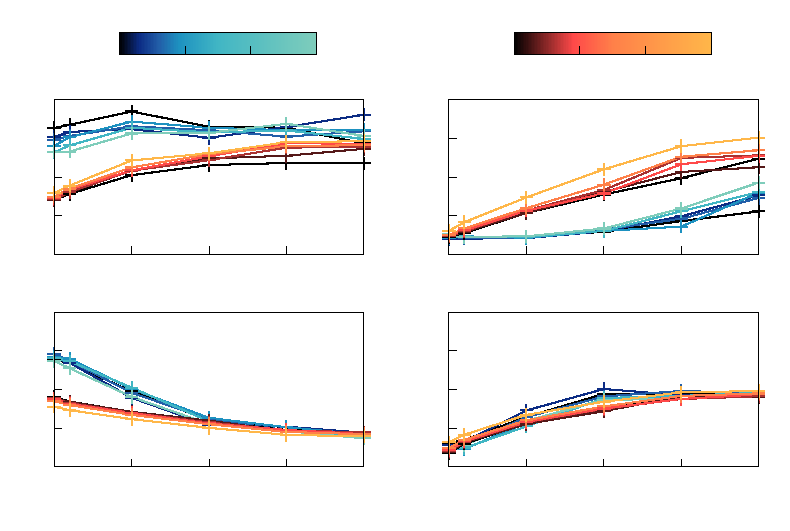
\includegraphics{licl-zif-hbonds-fit-pressure}}%
    \gplfronttext
  \end{picture}%
\endgroup

%     \caption{Variations of the time constant and weights of the bi-exponential
%     hydrogen bonds autocorrelation decay as function of the pressure in bulk
%     (blue shades) and confined (red shades) liquids.}
%     \label{fig:licl-zif:hbonds:fit:pressure}
% \end{figure}
%
% % \begin{figure}[ht]
% %     \centering
% %     % GNUPLOT: LaTeX picture with Postscript
\begingroup
  \makeatletter
  \providecommand\color[2][]{%
    \GenericError{(gnuplot) \space\space\space\@spaces}{%
      Package color not loaded in conjunction with
      terminal option `colourtext'%
    }{See the gnuplot documentation for explanation.%
    }{Either use 'blacktext' in gnuplot or load the package
      color.sty in LaTeX.}%
    \renewcommand\color[2][]{}%
  }%
  \providecommand\includegraphics[2][]{%
    \GenericError{(gnuplot) \space\space\space\@spaces}{%
      Package graphicx or graphics not loaded%
    }{See the gnuplot documentation for explanation.%
    }{The gnuplot epslatex terminal needs graphicx.sty or graphics.sty.}%
    \renewcommand\includegraphics[2][]{}%
  }%
  \providecommand\rotatebox[2]{#2}%
  \@ifundefined{ifGPcolor}{%
    \newif\ifGPcolor
    \GPcolortrue
  }{}%
  \@ifundefined{ifGPblacktext}{%
    \newif\ifGPblacktext
    \GPblacktextfalse
  }{}%
  % define a \g@addto@macro without @ in the name:
  \let\gplgaddtomacro\g@addto@macro
  % define empty templates for all commands taking text:
  \gdef\gplbacktext{}%
  \gdef\gplfronttext{}%
  \makeatother
  \ifGPblacktext
    % no textcolor at all
    \def\colorrgb#1{}%
    \def\colorgray#1{}%
  \else
    % gray or color?
    \ifGPcolor
      \def\colorrgb#1{\color[rgb]{#1}}%
      \def\colorgray#1{\color[gray]{#1}}%
      \expandafter\def\csname LTw\endcsname{\color{white}}%
      \expandafter\def\csname LTb\endcsname{\color{black}}%
      \expandafter\def\csname LTa\endcsname{\color{black}}%
      \expandafter\def\csname LT0\endcsname{\color[rgb]{1,0,0}}%
      \expandafter\def\csname LT1\endcsname{\color[rgb]{0,1,0}}%
      \expandafter\def\csname LT2\endcsname{\color[rgb]{0,0,1}}%
      \expandafter\def\csname LT3\endcsname{\color[rgb]{1,0,1}}%
      \expandafter\def\csname LT4\endcsname{\color[rgb]{0,1,1}}%
      \expandafter\def\csname LT5\endcsname{\color[rgb]{1,1,0}}%
      \expandafter\def\csname LT6\endcsname{\color[rgb]{0,0,0}}%
      \expandafter\def\csname LT7\endcsname{\color[rgb]{1,0.3,0}}%
      \expandafter\def\csname LT8\endcsname{\color[rgb]{0.5,0.5,0.5}}%
    \else
      % gray
      \def\colorrgb#1{\color{black}}%
      \def\colorgray#1{\color[gray]{#1}}%
      \expandafter\def\csname LTw\endcsname{\color{white}}%
      \expandafter\def\csname LTb\endcsname{\color{black}}%
      \expandafter\def\csname LTa\endcsname{\color{black}}%
      \expandafter\def\csname LT0\endcsname{\color{black}}%
      \expandafter\def\csname LT1\endcsname{\color{black}}%
      \expandafter\def\csname LT2\endcsname{\color{black}}%
      \expandafter\def\csname LT3\endcsname{\color{black}}%
      \expandafter\def\csname LT4\endcsname{\color{black}}%
      \expandafter\def\csname LT5\endcsname{\color{black}}%
      \expandafter\def\csname LT6\endcsname{\color{black}}%
      \expandafter\def\csname LT7\endcsname{\color{black}}%
      \expandafter\def\csname LT8\endcsname{\color{black}}%
    \fi
  \fi
    \setlength{\unitlength}{0.0500bp}%
    \ifx\gptboxheight\undefined%
      \newlength{\gptboxheight}%
      \newlength{\gptboxwidth}%
      \newsavebox{\gptboxtext}%
    \fi%
    \setlength{\fboxrule}{0.5pt}%
    \setlength{\fboxsep}{1pt}%
\begin{picture}(7580.00,3960.00)%
    \gplgaddtomacro\gplbacktext{%
      \csname LTb\endcsname%%
      \put(612,2352){\makebox(0,0)[r]{\strut{}$0$}}%
      \csname LTb\endcsname%%
      \put(612,2707){\makebox(0,0)[r]{\strut{}$1$}}%
      \csname LTb\endcsname%%
      \put(612,3063){\makebox(0,0)[r]{\strut{}$2$}}%
      \csname LTb\endcsname%%
      \put(612,3418){\makebox(0,0)[r]{\strut{}$3$}}%
      \csname LTb\endcsname%%
      \put(612,3773){\makebox(0,0)[r]{\strut{}$4$}}%
      \csname LTb\endcsname%%
      \put(714,2166){\makebox(0,0){\strut{}$0$}}%
      \csname LTb\endcsname%%
      \put(1406,2166){\makebox(0,0){\strut{}$5$}}%
      \csname LTb\endcsname%%
      \put(2099,2166){\makebox(0,0){\strut{}$10$}}%
      \csname LTb\endcsname%%
      \put(2791,2166){\makebox(0,0){\strut{}$15$}}%
      \csname LTb\endcsname%%
      \put(3483,2166){\makebox(0,0){\strut{}$20$}}%
    }%
    \gplgaddtomacro\gplfronttext{%
      \csname LTb\endcsname%%
      \put(222,3062){\rotatebox{-270}{\makebox(0,0){\strut{}$\tau_1$ (ps)}}}%
    }%
    \gplgaddtomacro\gplbacktext{%
      \csname LTb\endcsname%%
      \put(4402,2352){\makebox(0,0)[r]{\strut{}$0$}}%
      \csname LTb\endcsname%%
      \put(4402,2707){\makebox(0,0)[r]{\strut{}$20$}}%
      \csname LTb\endcsname%%
      \put(4402,3063){\makebox(0,0)[r]{\strut{}$40$}}%
      \csname LTb\endcsname%%
      \put(4402,3418){\makebox(0,0)[r]{\strut{}$60$}}%
      \csname LTb\endcsname%%
      \put(4402,3773){\makebox(0,0)[r]{\strut{}$80$}}%
      \csname LTb\endcsname%%
      \put(4504,2166){\makebox(0,0){\strut{}$0$}}%
      \csname LTb\endcsname%%
      \put(5196,2166){\makebox(0,0){\strut{}$5$}}%
      \csname LTb\endcsname%%
      \put(5889,2166){\makebox(0,0){\strut{}$10$}}%
      \csname LTb\endcsname%%
      \put(6581,2166){\makebox(0,0){\strut{}$15$}}%
      \csname LTb\endcsname%%
      \put(7273,2166){\makebox(0,0){\strut{}$20$}}%
    }%
    \gplgaddtomacro\gplfronttext{%
      \csname LTb\endcsname%%
      \put(3910,3062){\rotatebox{-270}{\makebox(0,0){\strut{}$\tau_2$ (ps)}}}%
      \csname LTb\endcsname%%
      \put(5422,3606){\makebox(0,0)[r]{\strut{}confined}}%
      \csname LTb\endcsname%%
      \put(5422,3420){\makebox(0,0)[r]{\strut{}bulk}}%
    }%
    \gplgaddtomacro\gplbacktext{%
      \csname LTb\endcsname%%
      \put(612,595){\makebox(0,0)[r]{\strut{}$0$}}%
      \csname LTb\endcsname%%
      \put(612,895){\makebox(0,0)[r]{\strut{}$25$}}%
      \csname LTb\endcsname%%
      \put(612,1195){\makebox(0,0)[r]{\strut{}$50$}}%
      \csname LTb\endcsname%%
      \put(612,1494){\makebox(0,0)[r]{\strut{}$75$}}%
      \csname LTb\endcsname%%
      \put(612,1794){\makebox(0,0)[r]{\strut{}$100$}}%
      \csname LTb\endcsname%%
      \put(714,409){\makebox(0,0){\strut{}$0$}}%
      \csname LTb\endcsname%%
      \put(1406,409){\makebox(0,0){\strut{}$5$}}%
      \csname LTb\endcsname%%
      \put(2099,409){\makebox(0,0){\strut{}$10$}}%
      \csname LTb\endcsname%%
      \put(2791,409){\makebox(0,0){\strut{}$15$}}%
      \csname LTb\endcsname%%
      \put(3483,409){\makebox(0,0){\strut{}$20$}}%
    }%
    \gplgaddtomacro\gplfronttext{%
      \csname LTb\endcsname%%
      \put(201,1194){\rotatebox{-270}{\makebox(0,0){\strut{}$A_1$ (\%)}}}%
      \csname LTb\endcsname%%
      \put(2098,130){\makebox(0,0){\strut{}\small concentration (mol/L)}}%
    }%
    \gplgaddtomacro\gplbacktext{%
      \csname LTb\endcsname%%
      \put(4402,595){\makebox(0,0)[r]{\strut{}$0$}}%
      \csname LTb\endcsname%%
      \put(4402,895){\makebox(0,0)[r]{\strut{}$25$}}%
      \csname LTb\endcsname%%
      \put(4402,1195){\makebox(0,0)[r]{\strut{}$50$}}%
      \csname LTb\endcsname%%
      \put(4402,1494){\makebox(0,0)[r]{\strut{}$75$}}%
      \csname LTb\endcsname%%
      \put(4402,1794){\makebox(0,0)[r]{\strut{}$100$}}%
      \csname LTb\endcsname%%
      \put(4504,409){\makebox(0,0){\strut{}$0$}}%
      \csname LTb\endcsname%%
      \put(5196,409){\makebox(0,0){\strut{}$5$}}%
      \csname LTb\endcsname%%
      \put(5889,409){\makebox(0,0){\strut{}$10$}}%
      \csname LTb\endcsname%%
      \put(6581,409){\makebox(0,0){\strut{}$15$}}%
      \csname LTb\endcsname%%
      \put(7273,409){\makebox(0,0){\strut{}$20$}}%
    }%
    \gplgaddtomacro\gplfronttext{%
      \csname LTb\endcsname%%
      \put(3991,1194){\rotatebox{-270}{\makebox(0,0){\strut{}$A_2$ (\%)}}}%
      \csname LTb\endcsname%%
      \put(5888,130){\makebox(0,0){\strut{}\small concentration (mol/L)}}%
    }%
    \gplbacktext
    \put(0,0){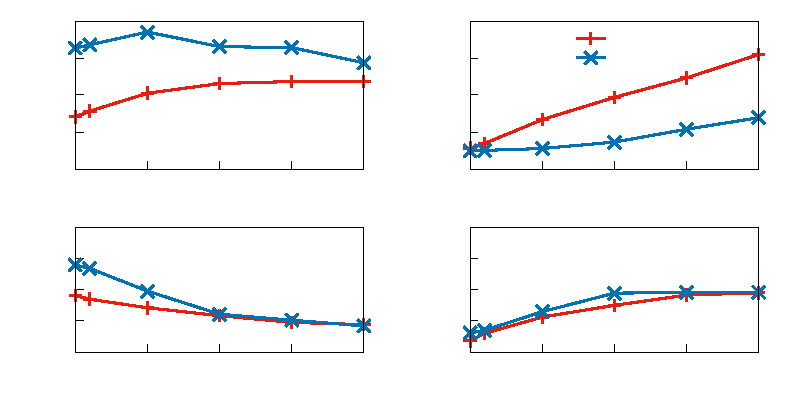
\includegraphics{licl-zif-hbonds-fit}}%
    \gplfronttext
  \end{picture}%
\endgroup

% %     \caption{Variations of the time constant and weights of the bi-exponential
% %     hydrogen bonds autocorrelation decay at \SI{0}{GPa} in bulk and confined
% %     liquid as function of the LiCl concentration.}
% %     \label{fig:licl-zif:hbonds:fit}
% % \end{figure}
%
% This geometric definition of hydrogen bonds has a minor inconvenient: small
% fluctuations of the atomic positions, near the cut-off values, can be mistaken
% for hydrogen bond forming and breaking. To overcome this issue, I also
% computed the time autocorrelation of the orientation vector $\vec u(t)$ of
% water molecules:
% \[C_{\text{rot}}(t) = \left\langle P_2(\vec u(t_0) \cdot \vec u(t_0 + t)) \right\rangle_{t_0} ,\]
% where $P_2(x)$ is the second order Legendre polynomial $P_2(x) = 1/2\ (3x^2 -
% 1)$\cite{Fogarty2014}. The resulting fit coefficients are presented in
% table~\ref{table:licl-zif:rotcf}. As water is a strongly associated liquid,
% breaking a hydrogen bond is predominantly correlated to rotational jumps, both
% autocorrelation decay in very similar ways, and I will mainly focus the
% discussion on hydrogen bonds dynamics.
%
% % \begin{figure}[ht]
% %     \centering
% %     % GNUPLOT: LaTeX picture with Postscript
\begingroup
  \makeatletter
  \providecommand\color[2][]{%
    \GenericError{(gnuplot) \space\space\space\@spaces}{%
      Package color not loaded in conjunction with
      terminal option `colourtext'%
    }{See the gnuplot documentation for explanation.%
    }{Either use 'blacktext' in gnuplot or load the package
      color.sty in LaTeX.}%
    \renewcommand\color[2][]{}%
  }%
  \providecommand\includegraphics[2][]{%
    \GenericError{(gnuplot) \space\space\space\@spaces}{%
      Package graphicx or graphics not loaded%
    }{See the gnuplot documentation for explanation.%
    }{The gnuplot epslatex terminal needs graphicx.sty or graphics.sty.}%
    \renewcommand\includegraphics[2][]{}%
  }%
  \providecommand\rotatebox[2]{#2}%
  \@ifundefined{ifGPcolor}{%
    \newif\ifGPcolor
    \GPcolortrue
  }{}%
  \@ifundefined{ifGPblacktext}{%
    \newif\ifGPblacktext
    \GPblacktextfalse
  }{}%
  % define a \g@addto@macro without @ in the name:
  \let\gplgaddtomacro\g@addto@macro
  % define empty templates for all commands taking text:
  \gdef\gplbacktext{}%
  \gdef\gplfronttext{}%
  \makeatother
  \ifGPblacktext
    % no textcolor at all
    \def\colorrgb#1{}%
    \def\colorgray#1{}%
  \else
    % gray or color?
    \ifGPcolor
      \def\colorrgb#1{\color[rgb]{#1}}%
      \def\colorgray#1{\color[gray]{#1}}%
      \expandafter\def\csname LTw\endcsname{\color{white}}%
      \expandafter\def\csname LTb\endcsname{\color{black}}%
      \expandafter\def\csname LTa\endcsname{\color{black}}%
      \expandafter\def\csname LT0\endcsname{\color[rgb]{1,0,0}}%
      \expandafter\def\csname LT1\endcsname{\color[rgb]{0,1,0}}%
      \expandafter\def\csname LT2\endcsname{\color[rgb]{0,0,1}}%
      \expandafter\def\csname LT3\endcsname{\color[rgb]{1,0,1}}%
      \expandafter\def\csname LT4\endcsname{\color[rgb]{0,1,1}}%
      \expandafter\def\csname LT5\endcsname{\color[rgb]{1,1,0}}%
      \expandafter\def\csname LT6\endcsname{\color[rgb]{0,0,0}}%
      \expandafter\def\csname LT7\endcsname{\color[rgb]{1,0.3,0}}%
      \expandafter\def\csname LT8\endcsname{\color[rgb]{0.5,0.5,0.5}}%
    \else
      % gray
      \def\colorrgb#1{\color{black}}%
      \def\colorgray#1{\color[gray]{#1}}%
      \expandafter\def\csname LTw\endcsname{\color{white}}%
      \expandafter\def\csname LTb\endcsname{\color{black}}%
      \expandafter\def\csname LTa\endcsname{\color{black}}%
      \expandafter\def\csname LT0\endcsname{\color{black}}%
      \expandafter\def\csname LT1\endcsname{\color{black}}%
      \expandafter\def\csname LT2\endcsname{\color{black}}%
      \expandafter\def\csname LT3\endcsname{\color{black}}%
      \expandafter\def\csname LT4\endcsname{\color{black}}%
      \expandafter\def\csname LT5\endcsname{\color{black}}%
      \expandafter\def\csname LT6\endcsname{\color{black}}%
      \expandafter\def\csname LT7\endcsname{\color{black}}%
      \expandafter\def\csname LT8\endcsname{\color{black}}%
    \fi
  \fi
    \setlength{\unitlength}{0.0500bp}%
    \ifx\gptboxheight\undefined%
      \newlength{\gptboxheight}%
      \newlength{\gptboxwidth}%
      \newsavebox{\gptboxtext}%
    \fi%
    \setlength{\fboxrule}{0.5pt}%
    \setlength{\fboxsep}{1pt}%
\begin{picture}(5660.00,5660.00)%
    \gplgaddtomacro\gplbacktext{%
      \csname LTb\endcsname%%
      \put(752,3264){\makebox(0,0)[r]{\strut{}$0$}}%
      \csname LTb\endcsname%%
      \put(752,3700){\makebox(0,0)[r]{\strut{}$0.2$}}%
      \csname LTb\endcsname%%
      \put(752,4135){\makebox(0,0)[r]{\strut{}$0.4$}}%
      \csname LTb\endcsname%%
      \put(752,4571){\makebox(0,0)[r]{\strut{}$0.6$}}%
      \csname LTb\endcsname%%
      \put(752,5006){\makebox(0,0)[r]{\strut{}$0.8$}}%
      \csname LTb\endcsname%%
      \put(752,5442){\makebox(0,0)[r]{\strut{}$1$}}%
      \csname LTb\endcsname%%
      \put(871,3047){\makebox(0,0){\strut{}$0$}}%
      \csname LTb\endcsname%%
      \put(1979,3047){\makebox(0,0){\strut{}$5$}}%
      \csname LTb\endcsname%%
      \put(3087,3047){\makebox(0,0){\strut{}$10$}}%
      \csname LTb\endcsname%%
      \put(4194,3047){\makebox(0,0){\strut{}$15$}}%
      \csname LTb\endcsname%%
      \put(5302,3047){\makebox(0,0){\strut{}$20$}}%
    }%
    \gplgaddtomacro\gplfronttext{%
      \csname LTb\endcsname%%
      \put(178,4353){\rotatebox{-270}{\makebox(0,0){\strut{}auto correlation}}}%
      \csname LTb\endcsname%%
      \put(2631,5247){\makebox(0,0)[r]{\strut{}0 mol/L}}%
      \csname LTb\endcsname%%
      \put(2631,5030){\makebox(0,0)[r]{\strut{}1 mol/L}}%
      \csname LTb\endcsname%%
      \put(2631,4813){\makebox(0,0)[r]{\strut{}5 mol/L}}%
      \csname LTb\endcsname%%
      \put(4383,5247){\makebox(0,0)[r]{\strut{}10 mol/L}}%
      \csname LTb\endcsname%%
      \put(4383,5030){\makebox(0,0)[r]{\strut{}15 mol/L}}%
      \csname LTb\endcsname%%
      \put(4383,4813){\makebox(0,0)[r]{\strut{}20 mol/L}}%
    }%
    \gplgaddtomacro\gplbacktext{%
      \csname LTb\endcsname%%
      \put(752,694){\makebox(0,0)[r]{\strut{}$0$}}%
      \csname LTb\endcsname%%
      \put(752,1078){\makebox(0,0)[r]{\strut{}$0.2$}}%
      \csname LTb\endcsname%%
      \put(752,1462){\makebox(0,0)[r]{\strut{}$0.4$}}%
      \csname LTb\endcsname%%
      \put(752,1845){\makebox(0,0)[r]{\strut{}$0.6$}}%
      \csname LTb\endcsname%%
      \put(752,2229){\makebox(0,0)[r]{\strut{}$0.8$}}%
      \csname LTb\endcsname%%
      \put(752,2613){\makebox(0,0)[r]{\strut{}$1$}}%
      \csname LTb\endcsname%%
      \put(871,477){\makebox(0,0){\strut{}$0$}}%
      \csname LTb\endcsname%%
      \put(1979,477){\makebox(0,0){\strut{}$5$}}%
      \csname LTb\endcsname%%
      \put(3087,477){\makebox(0,0){\strut{}$10$}}%
      \csname LTb\endcsname%%
      \put(4194,477){\makebox(0,0){\strut{}$15$}}%
      \csname LTb\endcsname%%
      \put(5302,477){\makebox(0,0){\strut{}$20$}}%
    }%
    \gplgaddtomacro\gplfronttext{%
      \csname LTb\endcsname%%
      \put(178,1653){\rotatebox{-270}{\makebox(0,0){\strut{}auto correlation}}}%
      \csname LTb\endcsname%%
      \put(3086,152){\makebox(0,0){\strut{}time (ps)}}%
    }%
    \gplbacktext
    \put(0,0){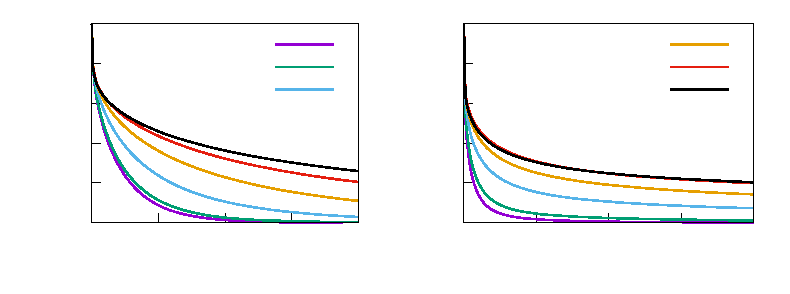
\includegraphics{licl-zif-rotcf}}%
    \gplfronttext
  \end{picture}%
\endgroup

% %     \caption{Rotational autocorrelation in bulk (left) and confined (right)
% %     electrolyte as function of LiCl concentration.}
% %     \label{fig:licl-zif:rotcf}
% % \end{figure}
%
% \begin{table}[ht]
%     \caption{Fit coefficients for the rotational autocorrelation decay at \SI{0}{GPa}.}
%     \label{table:licl-zif:rotcf}
%     \centering
%     \begin{tabular}{c c c c c c c c c c}
%         \toprule
%         \multicolumn{1}{c}{~} & \multicolumn{4}{c}{Bulk}                          &~& \multicolumn{4}{c}{Confined} \\
%         \multicolumn{1}{c}{~} & $\tau_1$ (ps) & $\tau_2$ (ps) & $A_1$   & $A_2$   &~& $\tau_1$ (ps) & $\tau_2$ (ps) & $A_1$   & $A_2$   \\
%         \midrule
%         \SI{0}{mol/L}         &    2.69       &    1.05       & 55.6 \% & 17.2 \% &~&    0.85       &     4.65      &  32.2 \% &  5.0  \% \\
%         \SI{1}{mol/L}         &    1.84       &    4.02       & 40.3 \% & 30.0 \% &~&    1.23       &     10.9      &  31.5 \% &  6.2  \% \\
%         \SI{5}{mol/L}         &    2.42       &    7.69       & 33.5 \% & 37.1 \% &~&    1.92       &     24.3      &  30.6 \% &  15.9 \% \\
%         \SI{10}{mol/L}        &    2.80       &    13.8       & 24.8 \% & 45.8 \% &~&    2.33       &     33.6      &  27.1 \% &  25.3 \% \\
%         \SI{15}{mol/L}        &    3.24       &    22.8       & 21.4 \% & 48.5 \% &~&    2.62       &     47.1      &  24.7 \% &  30.1 \% \\
%         \SI{20}{mol/L}        &    3.34       &    31.8       & 20.8 \% & 48.3 \% &~&    2.54       &     51.0      &  23.7 \% &  29.7 \% \\
%         \bottomrule
%     \end{tabular}
% \end{table}
%
% % \begin{figure}[ht]
% %     \centering
% %     % GNUPLOT: LaTeX picture with Postscript
\begingroup
  \makeatletter
  \providecommand\color[2][]{%
    \GenericError{(gnuplot) \space\space\space\@spaces}{%
      Package color not loaded in conjunction with
      terminal option `colourtext'%
    }{See the gnuplot documentation for explanation.%
    }{Either use 'blacktext' in gnuplot or load the package
      color.sty in LaTeX.}%
    \renewcommand\color[2][]{}%
  }%
  \providecommand\includegraphics[2][]{%
    \GenericError{(gnuplot) \space\space\space\@spaces}{%
      Package graphicx or graphics not loaded%
    }{See the gnuplot documentation for explanation.%
    }{The gnuplot epslatex terminal needs graphicx.sty or graphics.sty.}%
    \renewcommand\includegraphics[2][]{}%
  }%
  \providecommand\rotatebox[2]{#2}%
  \@ifundefined{ifGPcolor}{%
    \newif\ifGPcolor
    \GPcolortrue
  }{}%
  \@ifundefined{ifGPblacktext}{%
    \newif\ifGPblacktext
    \GPblacktextfalse
  }{}%
  % define a \g@addto@macro without @ in the name:
  \let\gplgaddtomacro\g@addto@macro
  % define empty templates for all commands taking text:
  \gdef\gplbacktext{}%
  \gdef\gplfronttext{}%
  \makeatother
  \ifGPblacktext
    % no textcolor at all
    \def\colorrgb#1{}%
    \def\colorgray#1{}%
  \else
    % gray or color?
    \ifGPcolor
      \def\colorrgb#1{\color[rgb]{#1}}%
      \def\colorgray#1{\color[gray]{#1}}%
      \expandafter\def\csname LTw\endcsname{\color{white}}%
      \expandafter\def\csname LTb\endcsname{\color{black}}%
      \expandafter\def\csname LTa\endcsname{\color{black}}%
      \expandafter\def\csname LT0\endcsname{\color[rgb]{1,0,0}}%
      \expandafter\def\csname LT1\endcsname{\color[rgb]{0,1,0}}%
      \expandafter\def\csname LT2\endcsname{\color[rgb]{0,0,1}}%
      \expandafter\def\csname LT3\endcsname{\color[rgb]{1,0,1}}%
      \expandafter\def\csname LT4\endcsname{\color[rgb]{0,1,1}}%
      \expandafter\def\csname LT5\endcsname{\color[rgb]{1,1,0}}%
      \expandafter\def\csname LT6\endcsname{\color[rgb]{0,0,0}}%
      \expandafter\def\csname LT7\endcsname{\color[rgb]{1,0.3,0}}%
      \expandafter\def\csname LT8\endcsname{\color[rgb]{0.5,0.5,0.5}}%
    \else
      % gray
      \def\colorrgb#1{\color{black}}%
      \def\colorgray#1{\color[gray]{#1}}%
      \expandafter\def\csname LTw\endcsname{\color{white}}%
      \expandafter\def\csname LTb\endcsname{\color{black}}%
      \expandafter\def\csname LTa\endcsname{\color{black}}%
      \expandafter\def\csname LT0\endcsname{\color{black}}%
      \expandafter\def\csname LT1\endcsname{\color{black}}%
      \expandafter\def\csname LT2\endcsname{\color{black}}%
      \expandafter\def\csname LT3\endcsname{\color{black}}%
      \expandafter\def\csname LT4\endcsname{\color{black}}%
      \expandafter\def\csname LT5\endcsname{\color{black}}%
      \expandafter\def\csname LT6\endcsname{\color{black}}%
      \expandafter\def\csname LT7\endcsname{\color{black}}%
      \expandafter\def\csname LT8\endcsname{\color{black}}%
    \fi
  \fi
    \setlength{\unitlength}{0.0500bp}%
    \ifx\gptboxheight\undefined%
      \newlength{\gptboxheight}%
      \newlength{\gptboxwidth}%
      \newsavebox{\gptboxtext}%
    \fi%
    \setlength{\fboxrule}{0.5pt}%
    \setlength{\fboxsep}{1pt}%
\begin{picture}(7580.00,5100.00)%
    \gplgaddtomacro\gplbacktext{%
      \csname LTb\endcsname%%
      \put(408,2667){\makebox(0,0)[r]{\strut{}$0$}}%
      \csname LTb\endcsname%%
      \put(408,3037){\makebox(0,0)[r]{\strut{}$1$}}%
      \csname LTb\endcsname%%
      \put(408,3408){\makebox(0,0)[r]{\strut{}$2$}}%
      \csname LTb\endcsname%%
      \put(408,3778){\makebox(0,0)[r]{\strut{}$3$}}%
      \csname LTb\endcsname%%
      \put(408,4148){\makebox(0,0)[r]{\strut{}$4$}}%
      \csname LTb\endcsname%%
      \put(510,2481){\makebox(0,0){\strut{}$0$}}%
      \csname LTb\endcsname%%
      \put(1253,2481){\makebox(0,0){\strut{}$5$}}%
      \csname LTb\endcsname%%
      \put(1997,2481){\makebox(0,0){\strut{}$10$}}%
      \csname LTb\endcsname%%
      \put(2740,2481){\makebox(0,0){\strut{}$15$}}%
      \csname LTb\endcsname%%
      \put(3483,2481){\makebox(0,0){\strut{}$20$}}%
    }%
    \gplgaddtomacro\gplfronttext{%
      \csname LTb\endcsname%%
      \put(120,3407){\rotatebox{-270}{\makebox(0,0){\strut{}$\tau_1$ (ps)}}}%
      \csname LTb\endcsname%%
      \put(1137,4440){\makebox(0,0){\strut{}\footnotesize 0}}%
      \csname LTb\endcsname%%
      \put(1768,4440){\makebox(0,0){\strut{}\footnotesize 0.33}}%
      \csname LTb\endcsname%%
      \put(2399,4440){\makebox(0,0){\strut{}\footnotesize 0.67}}%
      \csname LTb\endcsname%%
      \put(3031,4440){\makebox(0,0){\strut{}\footnotesize 1}}%
      \csname LTb\endcsname%%
      \put(2084,5016){\makebox(0,0){\strut{}\footnotesize bulk liquid pressure (GPa)}}%
    }%
    \gplgaddtomacro\gplbacktext{%
      \csname LTb\endcsname%%
      \put(4198,2667){\makebox(0,0)[r]{\strut{}$0$}}%
      \csname LTb\endcsname%%
      \put(4198,3037){\makebox(0,0)[r]{\strut{}$25$}}%
      \csname LTb\endcsname%%
      \put(4198,3408){\makebox(0,0)[r]{\strut{}$50$}}%
      \csname LTb\endcsname%%
      \put(4198,3778){\makebox(0,0)[r]{\strut{}$75$}}%
      \csname LTb\endcsname%%
      \put(4198,4148){\makebox(0,0)[r]{\strut{}$100$}}%
      \csname LTb\endcsname%%
      \put(4300,2481){\makebox(0,0){\strut{}$0$}}%
      \csname LTb\endcsname%%
      \put(5043,2481){\makebox(0,0){\strut{}$5$}}%
      \csname LTb\endcsname%%
      \put(5787,2481){\makebox(0,0){\strut{}$10$}}%
      \csname LTb\endcsname%%
      \put(6530,2481){\makebox(0,0){\strut{}$15$}}%
      \csname LTb\endcsname%%
      \put(7273,2481){\makebox(0,0){\strut{}$20$}}%
    }%
    \gplgaddtomacro\gplfronttext{%
      \csname LTb\endcsname%%
      \put(3808,3407){\rotatebox{-270}{\makebox(0,0){\strut{}$\tau_2$ (ps)}}}%
    }%
    \gplgaddtomacro\gplbacktext{%
      \csname LTb\endcsname%%
      \put(408,627){\makebox(0,0)[r]{\strut{}$0$}}%
      \csname LTb\endcsname%%
      \put(408,998){\makebox(0,0)[r]{\strut{}$25$}}%
      \csname LTb\endcsname%%
      \put(408,1368){\makebox(0,0)[r]{\strut{}$50$}}%
      \csname LTb\endcsname%%
      \put(408,1739){\makebox(0,0)[r]{\strut{}$75$}}%
      \csname LTb\endcsname%%
      \put(408,2109){\makebox(0,0)[r]{\strut{}$100$}}%
      \csname LTb\endcsname%%
      \put(510,441){\makebox(0,0){\strut{}$0$}}%
      \csname LTb\endcsname%%
      \put(1253,441){\makebox(0,0){\strut{}$5$}}%
      \csname LTb\endcsname%%
      \put(1997,441){\makebox(0,0){\strut{}$10$}}%
      \csname LTb\endcsname%%
      \put(2740,441){\makebox(0,0){\strut{}$15$}}%
      \csname LTb\endcsname%%
      \put(3483,441){\makebox(0,0){\strut{}$20$}}%
    }%
    \gplgaddtomacro\gplfronttext{%
      \csname LTb\endcsname%%
      \put(69,1368){\rotatebox{-270}{\makebox(0,0){\strut{}$A_1$ (\%)}}}%
      \csname LTb\endcsname%%
      \put(1996,162){\makebox(0,0){\strut{}\footnotesize concentration (mol/L)}}%
    }%
    \gplgaddtomacro\gplbacktext{%
      \csname LTb\endcsname%%
      \put(4198,627){\makebox(0,0)[r]{\strut{}$0$}}%
      \csname LTb\endcsname%%
      \put(4198,998){\makebox(0,0)[r]{\strut{}$25$}}%
      \csname LTb\endcsname%%
      \put(4198,1368){\makebox(0,0)[r]{\strut{}$50$}}%
      \csname LTb\endcsname%%
      \put(4198,1739){\makebox(0,0)[r]{\strut{}$75$}}%
      \csname LTb\endcsname%%
      \put(4198,2109){\makebox(0,0)[r]{\strut{}$100$}}%
      \csname LTb\endcsname%%
      \put(4300,441){\makebox(0,0){\strut{}$0$}}%
      \csname LTb\endcsname%%
      \put(5043,441){\makebox(0,0){\strut{}$5$}}%
      \csname LTb\endcsname%%
      \put(5787,441){\makebox(0,0){\strut{}$10$}}%
      \csname LTb\endcsname%%
      \put(6530,441){\makebox(0,0){\strut{}$15$}}%
      \csname LTb\endcsname%%
      \put(7273,441){\makebox(0,0){\strut{}$20$}}%
    }%
    \gplgaddtomacro\gplfronttext{%
      \csname LTb\endcsname%%
      \put(3808,1368){\rotatebox{-270}{\makebox(0,0){\strut{}$A_2$ (\%)}}}%
      \csname LTb\endcsname%%
      \put(5786,162){\makebox(0,0){\strut{}\footnotesize concentration (mol/L)}}%
    }%
    \gplgaddtomacro\gplbacktext{%
    }%
    \gplgaddtomacro\gplfronttext{%
      \csname LTb\endcsname%%
      \put(4926,4440){\makebox(0,0){\strut{}\footnotesize 0}}%
      \csname LTb\endcsname%%
      \put(5557,4440){\makebox(0,0){\strut{}\footnotesize 0.33}}%
      \csname LTb\endcsname%%
      \put(6188,4440){\makebox(0,0){\strut{}\footnotesize 0.67}}%
      \csname LTb\endcsname%%
      \put(6820,4440){\makebox(0,0){\strut{}\footnotesize 1}}%
      \csname LTb\endcsname%%
      \put(5873,5016){\makebox(0,0){\strut{}\footnotesize confined liquid pressure (GPa)}}%
    }%
    \gplgaddtomacro\gplbacktext{%
    }%
    \gplgaddtomacro\gplfronttext{%
    }%
    \gplgaddtomacro\gplbacktext{%
    }%
    \gplgaddtomacro\gplfronttext{%
    }%
    \gplgaddtomacro\gplbacktext{%
    }%
    \gplgaddtomacro\gplfronttext{%
    }%
    \gplbacktext
    \put(0,0){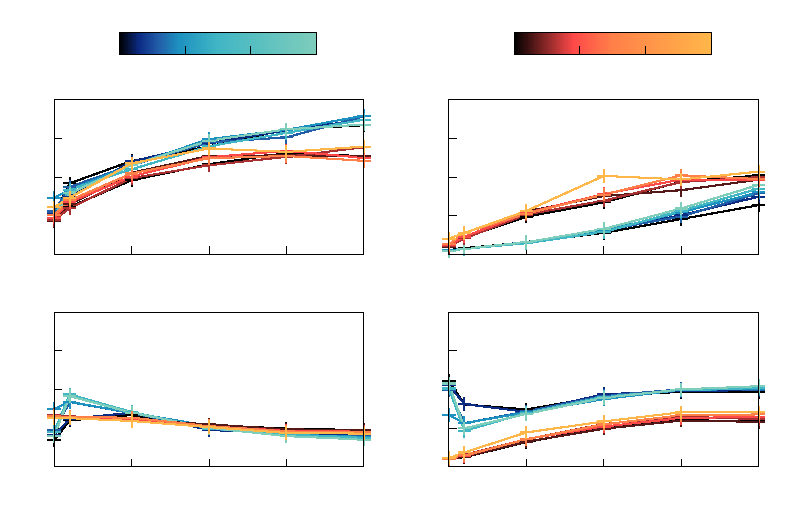
\includegraphics{licl-zif-rotcf-fit-pressure}}%
    \gplfronttext
  \end{picture}%
\endgroup

% %     \caption{Variations of the time constant and weights of the bi-exponential
% %     rotational autocorrelation decay as function of the pressure in bulk
% %     (blue shades) and confined (red shades) liquids.}
% %     \label{fig:licl-zif:rotcf:fit:pressure}
% % \end{figure}
%
% In the bulk liquid, the shortest lifetime is almost constant around \SI{3}{ps}
% as the concentration increases, but the weight of this fast process ($A_1$)
% decreases. This suggests that this fastest lifetime is associated with hydrogen
% bonds between water molecules surrounded only by other water molecules. As more
% and more ions are added in the system, water molecules are less likely to be
% surrounded only by other water molecules --- as is indicated by the results I
% presented in section~\ref{sec:licl-zifliquid-structure}. This lifetime is smaller in the
% confined liquid than it is in the bulk phase, which has already been shown for
% water at interfaces: \citeauthor{Fogarty2014}\cite{Fogarty2014} showed that it
% is linked to the librational motions of the OH bonds, and the dynamics of these
% \emph{dangling} OH groups at interfaces is faster than bulk\cite{Scatena2001}.
% On the other hand, the second lifetime, associated to the slowest process,
% increases with concentration, as well as the corresponding weight ($A_2$). This
% points to hydrogen bonds between water molecules bounded to ions.
%
% In the confined liquid, weights still evolve in the same way with respect to the
% concentration, which point to them being associated with the same kind of
% hydrogen bonds. The second lifetime increases in the confined liquid compared to
% the bulk liquid. This slowdown of water dynamics under confinement is
% well-known\cite{Fogarty2014}, and has been observed in many classes of
% nanoporous materials\cite{Jeffery2004, RomeroVargasCastrillon2009, Haigis2013,
% Scalfi2018}. It is attributed to the stronger organization of water as well as
% water molecules finding fewer partners for hydrogen bond exchange. The same
% arguments also apply to the increase in LiCl concentration, both in the bulk and
% confined liquid. This is coherent with what we see on the changes on bulk
% modulus as concentration changes in table~\ref{table:bulk}.
%
% \subsection{Deformation of the framework}
% \label{sec:licl-zifdeformation}
%
% \begin{figure}[ht]
%     \centering
%     % GNUPLOT: LaTeX picture with Postscript
\begingroup
  \makeatletter
  \providecommand\color[2][]{%
    \GenericError{(gnuplot) \space\space\space\@spaces}{%
      Package color not loaded in conjunction with
      terminal option `colourtext'%
    }{See the gnuplot documentation for explanation.%
    }{Either use 'blacktext' in gnuplot or load the package
      color.sty in LaTeX.}%
    \renewcommand\color[2][]{}%
  }%
  \providecommand\includegraphics[2][]{%
    \GenericError{(gnuplot) \space\space\space\@spaces}{%
      Package graphicx or graphics not loaded%
    }{See the gnuplot documentation for explanation.%
    }{The gnuplot epslatex terminal needs graphicx.sty or graphics.sty.}%
    \renewcommand\includegraphics[2][]{}%
  }%
  \providecommand\rotatebox[2]{#2}%
  \@ifundefined{ifGPcolor}{%
    \newif\ifGPcolor
    \GPcolortrue
  }{}%
  \@ifundefined{ifGPblacktext}{%
    \newif\ifGPblacktext
    \GPblacktextfalse
  }{}%
  % define a \g@addto@macro without @ in the name:
  \let\gplgaddtomacro\g@addto@macro
  % define empty templates for all commands taking text:
  \gdef\gplbacktext{}%
  \gdef\gplfronttext{}%
  \makeatother
  \ifGPblacktext
    % no textcolor at all
    \def\colorrgb#1{}%
    \def\colorgray#1{}%
  \else
    % gray or color?
    \ifGPcolor
      \def\colorrgb#1{\color[rgb]{#1}}%
      \def\colorgray#1{\color[gray]{#1}}%
      \expandafter\def\csname LTw\endcsname{\color{white}}%
      \expandafter\def\csname LTb\endcsname{\color{black}}%
      \expandafter\def\csname LTa\endcsname{\color{black}}%
      \expandafter\def\csname LT0\endcsname{\color[rgb]{1,0,0}}%
      \expandafter\def\csname LT1\endcsname{\color[rgb]{0,1,0}}%
      \expandafter\def\csname LT2\endcsname{\color[rgb]{0,0,1}}%
      \expandafter\def\csname LT3\endcsname{\color[rgb]{1,0,1}}%
      \expandafter\def\csname LT4\endcsname{\color[rgb]{0,1,1}}%
      \expandafter\def\csname LT5\endcsname{\color[rgb]{1,1,0}}%
      \expandafter\def\csname LT6\endcsname{\color[rgb]{0,0,0}}%
      \expandafter\def\csname LT7\endcsname{\color[rgb]{1,0.3,0}}%
      \expandafter\def\csname LT8\endcsname{\color[rgb]{0.5,0.5,0.5}}%
    \else
      % gray
      \def\colorrgb#1{\color{black}}%
      \def\colorgray#1{\color[gray]{#1}}%
      \expandafter\def\csname LTw\endcsname{\color{white}}%
      \expandafter\def\csname LTb\endcsname{\color{black}}%
      \expandafter\def\csname LTa\endcsname{\color{black}}%
      \expandafter\def\csname LT0\endcsname{\color{black}}%
      \expandafter\def\csname LT1\endcsname{\color{black}}%
      \expandafter\def\csname LT2\endcsname{\color{black}}%
      \expandafter\def\csname LT3\endcsname{\color{black}}%
      \expandafter\def\csname LT4\endcsname{\color{black}}%
      \expandafter\def\csname LT5\endcsname{\color{black}}%
      \expandafter\def\csname LT6\endcsname{\color{black}}%
      \expandafter\def\csname LT7\endcsname{\color{black}}%
      \expandafter\def\csname LT8\endcsname{\color{black}}%
    \fi
  \fi
    \setlength{\unitlength}{0.0500bp}%
    \ifx\gptboxheight\undefined%
      \newlength{\gptboxheight}%
      \newlength{\gptboxwidth}%
      \newsavebox{\gptboxtext}%
    \fi%
    \setlength{\fboxrule}{0.5pt}%
    \setlength{\fboxsep}{1pt}%
\begin{picture}(5660.00,3400.00)%
    \gplgaddtomacro\gplbacktext{%
      \csname LTb\endcsname%%
      \put(297,477){\makebox(0,0){\strut{}$0$}}%
      \csname LTb\endcsname%%
      \put(1298,477){\makebox(0,0){\strut{}$10$}}%
      \csname LTb\endcsname%%
      \put(2299,477){\makebox(0,0){\strut{}$20$}}%
      \csname LTb\endcsname%%
      \put(3300,477){\makebox(0,0){\strut{}$30$}}%
      \csname LTb\endcsname%%
      \put(4301,477){\makebox(0,0){\strut{}$40$}}%
      \csname LTb\endcsname%%
      \put(5302,477){\makebox(0,0){\strut{}$50$}}%
    }%
    \gplgaddtomacro\gplfronttext{%
      \csname LTb\endcsname%%
      \put(2799,152){\makebox(0,0){\strut{}$\phi$ (°)}}%
      \csname LTb\endcsname%%
      \put(4383,2987){\makebox(0,0)[r]{\strut{}0 mol/L}}%
      \csname LTb\endcsname%%
      \put(4383,2770){\makebox(0,0)[r]{\strut{}1 mol/L}}%
      \csname LTb\endcsname%%
      \put(4383,2553){\makebox(0,0)[r]{\strut{}5 mol/L}}%
      \csname LTb\endcsname%%
      \put(4383,2336){\makebox(0,0)[r]{\strut{}10 mol/L}}%
      \csname LTb\endcsname%%
      \put(4383,2119){\makebox(0,0)[r]{\strut{}15 mol/L}}%
      \csname LTb\endcsname%%
      \put(4383,1902){\makebox(0,0)[r]{\strut{}20 mol/L}}%
      \csname LTb\endcsname%%
      \put(4383,1685){\makebox(0,0)[r]{\strut{}empty}}%
    }%
    \gplbacktext
    \put(0,0){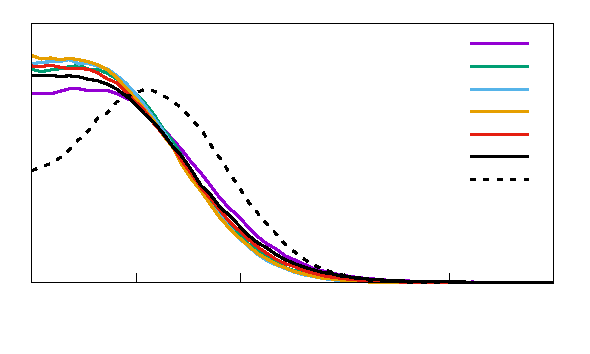
\includegraphics{licl-zif-dihedrals}}%
    \gplfronttext
  \end{picture}%
\endgroup

%     \caption{Swing dihedral angle distribution in empty and intruded \ZIF8 at
%     all the LiCl concentrations.}
%     \label{fig:licl-zif:dihedrals}
% \end{figure}
%
% So far, I have studied the property of the confined liquid inside the \ZIF8
% framework, and the changes in the structure and dynamic of this liquid as it
% goes from a bulk to a confined state. It is also interesting to look at the
% changes the framework undergoes when going from an empty state to an intruded
% state. Macroscopic changes to the volume are relatively small (less than 4\%),
% and presented in the next section, specially in figure~\ref{fig:licl-zif:pv}. In
% this section I will look at the internal deformations of the framework under
% intrusion. I used the distribution of the \ce{Zn-Zn-Zn-CH3} dihedral swing angle
% to characterize the deformations of the framework under intrusion. The
% distributions for empty and intruded \ZIF8 are presented in
% figure~\ref{fig:licl-zif:dihedrals}.
%
% The distribution for the empty framework reproduces the results from
% chapter~\ref{sec:ab-initio}: it is a Gaussian distribution, centered around the
% equilibrium value of 15°, and with fluctuations of the order of 10°. The
% distributions for \ZIF8 containing the electrolyte liquid does not seems to
% depend on the electrolyte concentration. Instead they are all centered around
% 5°, and still have the same order of magnitude for fluctuations. This is to be
% contrasted with the effect of nitrogen adsorption at \SI{77}{K} in \ZIF8; where
% the equilibrium value goes from 10° to 25° as the pores fill up with nitrogen.
% It is however interesting to note that the presence of ions does not impact the
% structure more than the presence of pure water does. This is coherent with the
% results presented in figure~\ref{fig:licl-zif:density}, where the water
% molecules are located inside the 6-member windows. Water molecules take the
% place of linkers that rotate to accommodate them in the windows. As ions never
% enter this window, they don't have any effect on the linkers rotation.
%
% \subsection{Elastic properties}
%
% \begin{figure}[ht]
%     \centering
%     % GNUPLOT: LaTeX picture with Postscript
\begingroup
  \makeatletter
  \providecommand\color[2][]{%
    \GenericError{(gnuplot) \space\space\space\@spaces}{%
      Package color not loaded in conjunction with
      terminal option `colourtext'%
    }{See the gnuplot documentation for explanation.%
    }{Either use 'blacktext' in gnuplot or load the package
      color.sty in LaTeX.}%
    \renewcommand\color[2][]{}%
  }%
  \providecommand\includegraphics[2][]{%
    \GenericError{(gnuplot) \space\space\space\@spaces}{%
      Package graphicx or graphics not loaded%
    }{See the gnuplot documentation for explanation.%
    }{The gnuplot epslatex terminal needs graphicx.sty or graphics.sty.}%
    \renewcommand\includegraphics[2][]{}%
  }%
  \providecommand\rotatebox[2]{#2}%
  \@ifundefined{ifGPcolor}{%
    \newif\ifGPcolor
    \GPcolortrue
  }{}%
  \@ifundefined{ifGPblacktext}{%
    \newif\ifGPblacktext
    \GPblacktextfalse
  }{}%
  % define a \g@addto@macro without @ in the name:
  \let\gplgaddtomacro\g@addto@macro
  % define empty templates for all commands taking text:
  \gdef\gplbacktext{}%
  \gdef\gplfronttext{}%
  \makeatother
  \ifGPblacktext
    % no textcolor at all
    \def\colorrgb#1{}%
    \def\colorgray#1{}%
  \else
    % gray or color?
    \ifGPcolor
      \def\colorrgb#1{\color[rgb]{#1}}%
      \def\colorgray#1{\color[gray]{#1}}%
      \expandafter\def\csname LTw\endcsname{\color{white}}%
      \expandafter\def\csname LTb\endcsname{\color{black}}%
      \expandafter\def\csname LTa\endcsname{\color{black}}%
      \expandafter\def\csname LT0\endcsname{\color[rgb]{1,0,0}}%
      \expandafter\def\csname LT1\endcsname{\color[rgb]{0,1,0}}%
      \expandafter\def\csname LT2\endcsname{\color[rgb]{0,0,1}}%
      \expandafter\def\csname LT3\endcsname{\color[rgb]{1,0,1}}%
      \expandafter\def\csname LT4\endcsname{\color[rgb]{0,1,1}}%
      \expandafter\def\csname LT5\endcsname{\color[rgb]{1,1,0}}%
      \expandafter\def\csname LT6\endcsname{\color[rgb]{0,0,0}}%
      \expandafter\def\csname LT7\endcsname{\color[rgb]{1,0.3,0}}%
      \expandafter\def\csname LT8\endcsname{\color[rgb]{0.5,0.5,0.5}}%
    \else
      % gray
      \def\colorrgb#1{\color{black}}%
      \def\colorgray#1{\color[gray]{#1}}%
      \expandafter\def\csname LTw\endcsname{\color{white}}%
      \expandafter\def\csname LTb\endcsname{\color{black}}%
      \expandafter\def\csname LTa\endcsname{\color{black}}%
      \expandafter\def\csname LT0\endcsname{\color{black}}%
      \expandafter\def\csname LT1\endcsname{\color{black}}%
      \expandafter\def\csname LT2\endcsname{\color{black}}%
      \expandafter\def\csname LT3\endcsname{\color{black}}%
      \expandafter\def\csname LT4\endcsname{\color{black}}%
      \expandafter\def\csname LT5\endcsname{\color{black}}%
      \expandafter\def\csname LT6\endcsname{\color{black}}%
      \expandafter\def\csname LT7\endcsname{\color{black}}%
      \expandafter\def\csname LT8\endcsname{\color{black}}%
    \fi
  \fi
    \setlength{\unitlength}{0.0500bp}%
    \ifx\gptboxheight\undefined%
      \newlength{\gptboxheight}%
      \newlength{\gptboxwidth}%
      \newsavebox{\gptboxtext}%
    \fi%
    \setlength{\fboxrule}{0.5pt}%
    \setlength{\fboxsep}{1pt}%
\begin{picture}(5660.00,6800.00)%
    \gplgaddtomacro\gplbacktext{%
      \csname LTb\endcsname%%
      \put(595,4094){\makebox(0,0)[r]{\strut{}$15$}}%
      \csname LTb\endcsname%%
      \put(595,4716){\makebox(0,0)[r]{\strut{}$20$}}%
      \csname LTb\endcsname%%
      \put(595,5338){\makebox(0,0)[r]{\strut{}$25$}}%
      \csname LTb\endcsname%%
      \put(595,5960){\makebox(0,0)[r]{\strut{}$30$}}%
      \csname LTb\endcsname%%
      \put(595,6582){\makebox(0,0)[r]{\strut{}$35$}}%
      \csname LTb\endcsname%%
      \put(923,3877){\makebox(0,0){\strut{}$0$}}%
      \csname LTb\endcsname%%
      \put(1965,3877){\makebox(0,0){\strut{}$0.25$}}%
      \csname LTb\endcsname%%
      \put(3008,3877){\makebox(0,0){\strut{}$0.5$}}%
      \csname LTb\endcsname%%
      \put(4051,3877){\makebox(0,0){\strut{}$0.75$}}%
      \csname LTb\endcsname%%
      \put(5093,3877){\makebox(0,0){\strut{}$1$}}%
    }%
    \gplgaddtomacro\gplfronttext{%
      \csname LTb\endcsname%%
      \put(140,5338){\rotatebox{-270}{\makebox(0,0){\strut{}volume (\si{nm^3})}}}%
      \csname LTb\endcsname%%
      \put(3008,3552){\makebox(0,0){\strut{}pressure (GPa)}}%
      \csname LTb\endcsname%%
      \put(2631,6387){\makebox(0,0)[r]{\strut{}0 mol/L}}%
      \csname LTb\endcsname%%
      \put(2631,6170){\makebox(0,0)[r]{\strut{}1 mol/L}}%
      \csname LTb\endcsname%%
      \put(2631,5953){\makebox(0,0)[r]{\strut{}5 mol/L}}%
      \csname LTb\endcsname%%
      \put(4383,6387){\makebox(0,0)[r]{\strut{}10 mol/L}}%
      \csname LTb\endcsname%%
      \put(4383,6170){\makebox(0,0)[r]{\strut{}15 mol/L}}%
      \csname LTb\endcsname%%
      \put(4383,5953){\makebox(0,0)[r]{\strut{}20 mol/L}}%
    }%
    \gplgaddtomacro\gplbacktext{%
      \csname LTb\endcsname%%
      \put(595,694){\makebox(0,0)[r]{\strut{}$110$}}%
      \csname LTb\endcsname%%
      \put(595,1316){\makebox(0,0)[r]{\strut{}$120$}}%
      \csname LTb\endcsname%%
      \put(595,1939){\makebox(0,0)[r]{\strut{}$130$}}%
      \csname LTb\endcsname%%
      \put(595,2561){\makebox(0,0)[r]{\strut{}$140$}}%
      \csname LTb\endcsname%%
      \put(595,3183){\makebox(0,0)[r]{\strut{}$150$}}%
      \csname LTb\endcsname%%
      \put(923,477){\makebox(0,0){\strut{}$0$}}%
      \csname LTb\endcsname%%
      \put(1965,477){\makebox(0,0){\strut{}$0.25$}}%
      \csname LTb\endcsname%%
      \put(3008,477){\makebox(0,0){\strut{}$0.5$}}%
      \csname LTb\endcsname%%
      \put(4051,477){\makebox(0,0){\strut{}$0.75$}}%
      \csname LTb\endcsname%%
      \put(5093,477){\makebox(0,0){\strut{}$1$}}%
    }%
    \gplgaddtomacro\gplfronttext{%
      \csname LTb\endcsname%%
      \put(21,1938){\rotatebox{-270}{\makebox(0,0){\strut{}volume (\si{nm^3})}}}%
      \csname LTb\endcsname%%
      \put(3008,152){\makebox(0,0){\strut{}pressure (GPa)}}%
      \csname LTb\endcsname%%
      \put(4383,2988){\makebox(0,0)[r]{\strut{}empty}}%
    }%
    \gplbacktext
    \put(0,0){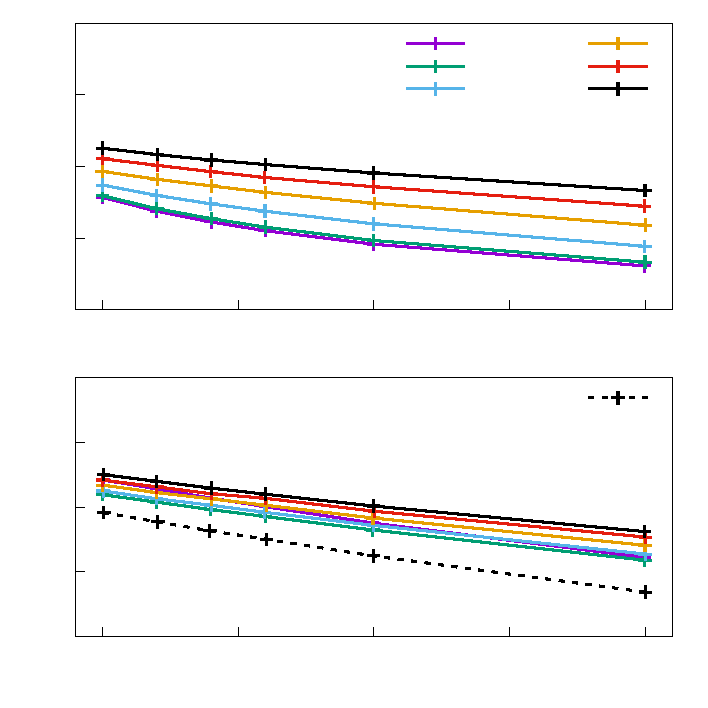
\includegraphics{licl-zif-pv}}%
    \gplfronttext
  \end{picture}%
\endgroup

%     \caption{Deformation of bulk liquid (top) and \ZIF8 with confined electrolyte
%     (bottom) as function of the pressure. Lines connect the different simulations
%     using the same concentration.}
%     \label{fig:licl-zif:pv}
% \end{figure}
%
% Given its potential applications in mechanical energy storage, one of the most
% important properties of the \ZIF8/electrolyte system is its mechanical behavior,
% and notably its stability under high pressure. As an increasing stress is
% applied to a material, it will first deform in a reversible and linear fashion,
% in what is called the linear elastic regime. Under higher stress, the
% material will start to deform in an irreversible way, and finally break.
% Information on the linear elastic regime and its extent is useful to study the
% stability of materials under stress, as stiffer materials are generally tougher
% and able to bear higher stress before failing. This is particularly important
% for soft nanoporous materials, where the mechanical stability range is lower
% than in inorganic porous materials such as zeolites, and where pressure-induced
% amorphization is common at moderate (sub-gigapascal)
% pressures\cite{Bennett2011, Cao2012, AOrtiz2013}.
%
% I probed the mechanical response of the \ZIF8/electrolyte system using direct
% simulations of the system under explicit hydrostatic stress. We can first note
% that even though I allowed arbitrary changes to the unit cell lengths and tilt
% factors, all the simulations cells remained orthorhombic. The
% figure~\ref{fig:licl-zif:pv} present the changes in volume as the pressure
% increases, for all the liquid concentrations. We can see that up to \SI{1}{GPa},
% the deformation remains in the elastic regime, and that the response is almost
% linear. Moreover, confining an electrolyte in the \ZIF8 structure do not
% drastically affect the mechanical properties of the system.
%
% From these curves, I extracted the bulk modulus $K$ of the system, defined as
% \[K = -V\left(\frac{\partial P}{\partial V}\right)_{N,T}\]
% The values obtained for all concentrations are reported in
% table~\ref{table:bulk}. The value for the empty \ZIF8 is close to the
% experimental\cite{Tan2012} value of \SI{7.8}{GPa}. The bulk modulii of pure
% water and \SI{1}{mol/L} are further away from the experimental
% values\cite{Lanman1934} of \SI{2.4}{GPa} and \SI{2.6}{GPa} respectively. These
% differences are likely coming from the force-fields we used, which were not
% parameterized on mechanical properties of the framework or the liquids.
%
% \begin{table}[ht]
%     \caption{Bulk modulus of the bulk electrolyte liquids and of \ZIF8
%     containing a confined electrolyte liquid.}
%     \label{table:bulk}
%     \centering
%     \renewcommand{\arraystretch}{1.1}
%     \begin{tabular}{c c c}
%         \toprule
%         Concentration   & Bulk liquid  & Liquid $\in$ \ZIF8 \\
%         \midrule
%         \SI{0}{mol/L}   &    4.3 GPa   &  11.2 GPa    \\
%         \SI{1}{mol/L}   &    4.4 GPa   &  13.0 GPa    \\
%         \SI{5}{mol/L}   &    5.0 GPa   &  13.6 GPa    \\
%         \SI{10}{mol/L}  &    6.1 GPa   &  14.4 GPa    \\
%         \SI{15}{mol/L}  &    7.2 GPa   &  15.2 GPa    \\
%         \SI{20}{mol/L}  &    8.4 GPa   &  15.4 GPa    \\
%         \bottomrule
%         Empty \ZIF8     &              &  10.5 GPa     \\
%         \bottomrule
%     \end{tabular}
% \end{table}
%
% The trends, however, are interesting to see. Adding water to the pores of \ZIF8
% only changes the bulk modulus by a moderate amount (10\%), meaning that most of
% the stiffness comes from the \ZIF8 framework --- the stiffer component of the
% two. However, adding ions to the liquid has a larger effect, both in the bulk
% state and the confined state, with the bulk modulus increasing by up to 50\% at
% \SI{20}{mol/L} with respect to the empty framework. Since I generated the
% structures in such a way that the volume occupied by the liquid is always the
% same, the increase in bulk modulus is not be related to changes in the size
% occupied by the ions relatively to water. Rather, this increase in bulk modulus
% comes from the stronger interactions between ions and water molecules, compared
% to interactions between water molecules. The interactions between lithium
% cations and water molecules are stronger than water--water hydrogen bonds, and
% will make the liquid less compressible, especially at high concentration where,
% statistically, all water molecules are bonded to at least one lithium atom. This
% is further supported by the fact that the bulk modulus increases by the same
% order of magnitude ($\approx$ \SI{5}{GPa}) in both the bulk liquid and the
% confined liquid in \ZIF8.
%
% \subsection{Thermodynamics of the intrusion}
%
% In order to shed light into the thermodynamics of electrolyte intrusion in
% \ZIF8, I extracted the potential energy for various sub-components of the total
% system by taking the average value of the interaction energy of the
% corresponding sub-components. The resulting average energies are presented in
% table~\ref{table:thermo:raw}; where $E_\text{total}$ is the total potential
% energy of the electrolyte confined in \ZIF8; $E_\text{ZIF}$ is the interaction
% of \ZIF8 with itself; $E_\text{LiCl}$ is the interaction of the confined
% electrolyte with itself; and $E_\text{ZIF/LiCl}$ is the interaction of the
% electrolyte with the \ZIF8. $E_\text{LiCl}^\text{bulk}$ refers to the total
% potential energy of the bulk electrolyte with the same number of particles as
% the confined one. Every quantity is expressed for one unit cell of \ZIF8, plus
% the confined liquid inside.
%
% \begin{table}[ht]
%     \caption{Average interaction energy in kcal/mol per unit cell for various
%     sub-systems. See the text for the definition of each sub-system.
%     For reference, $k_BT$ is \SI{0.6}{kcal/mol} at \SI{300}{K}.}
%     \label{table:thermo:raw}
%     \centering
%     \renewcommand{\arraystretch}{1.1}
%     \begin{tabular}{c c c c c c}
%         \toprule
%         Concentration  & $E_\text{Total}$ & $E_\text{ZIF}$ & $E_\text{LiCl}$ & $E_\text{LiCl/ZIF}$ & $E_\text{LiCl}^\text{bulk}$ \\
%         \midrule
%         \SI{0}{mol/L}  &     $-1617$        &    $-758.1$      &   $-703.1$        &     $-155.5$           &   $-822.9$    \\
%         \SI{1}{mol/L}  &     $-1859$        &    $-739.5$      &   $-974.0$        &     $-145.8$          &   $-1080$     \\
%         \SI{5}{mol/L}  &     $-2753$        &    $-738.3$      &   $-1864$         &     $-149.7$           &   $-1995$     \\
%         \SI{10}{mol/L} &     $-3628$        &    $-735.5$      &   $-2744$         &     $-148.6$           &   $-2898$     \\
%         \SI{15}{mol/L} &     $-4295$        &    $-732.5$      &   $-3416$         &     $-146.0$           &   $-3581$     \\
%         \SI{20}{mol/L} &     $-4818$        &    $-728.4$      &   $-3949$         &     $-140.9$           &   $-4117$     \\
%         \bottomrule
%         Empty          &     $-746.8$       &    $-746.8$      &                 &                      &             \\
%         \bottomrule
%     \end{tabular}
% \end{table}
%
% From these values, I can extract a few thermodynamic quantities of interest,
% presented in table~\ref{table:thermo}:
% \[\begin{aligned}
%     \Delta E_\text{ZIF} (c)  &= E_\text{ZIF}(c) - E_\text{ZIF}^\text{empty};\\
%     \Delta E_\text{LiCl} (c) &= E_\text{LiCl}(c) - E_\text{LiCl}^\text{bulk}(c);\\
%     \Delta H_\text{intr} (c) &= E_\text{total}(c) - E_\text{LiCl}^\text{bulk}(c) - E_\text{ZIF}^\text{empty}.\\
% \end{aligned}\]
% $\Delta E_\text{ZIF}$ is the energetic change in \ZIF8 during intrusion; $\Delta
% E_\text{LiCl}$ is the energetic change in the electrolyte during intrusion; and
% $\Delta H_\text{intr}$ is the intrusion enthalpy, \emph{i.e.} the enthalpy
% change during the \mbox{\ZIF8 + liquid $\rightarrow$ liquid $\in$
% \ZIF8} process. The sign convention is taken so that all of these energies are
% negative when the confined state is more stable.
%
% \begin{table}[ht]
%     \caption{Derived thermodynamic quantities in kcal/mol per unit cell. See
%     the text for the definition of each quantity.}
%     \label{table:thermo}
%     \centering
%     \renewcommand{\arraystretch}{1.3}
%     \begin{tabular}{c | c c c }
%         \toprule
%         Concentration  & $\Delta E_\text{ZIF}$ & $\Delta E_\text{LiCl}$ & $\Delta H_\text{intr}$ \\
%         \midrule
%         \SI{0}{mol/L}  &    $-11.3$            &    $-120$                &    $-47.3$               \\
%         \SI{1}{mol/L}  &       7.3             &    $-106$                &    $-32.2$               \\
%         \SI{5}{mol/L}  &       8.5             &    $-131$                &    $-11.2$               \\
%         \SI{10}{mol/L} &      11.3             &    $-154$                &     16.8               \\
%         \SI{15}{mol/L} &      14.3             &    $-165$                &     32.8               \\
%         \SI{20}{mol/L} &      18.4             &    $-168$                &     45.8               \\
%         \bottomrule
%     \end{tabular}
% \end{table}
%
% We can see in table~\ref{table:thermo} that the intrusion process has a
% relatively small impact on the ZIF: the energy difference between the empty and
% intruded states $\Delta E_\text{ZIF}$ is in the range of tens of $kT$ (at \SI{300}{K},
% $kT \approx \SI{0.6}{kcal/mol}$). The \ZIF8 framework is slightly destabilized
% (energetically) in presence of the intruded liquid except at \SI{0}{mol/L},
% where it is slightly stabilized. The overall effect is small compared to the two
% next trends we see. I have already shown that the presence of ions have little
% to no effect on the \ZIF8 structure in section~\ref{sec:licl-zifdeformation}.
%
% First, the liquid is always more energetically stable in the intruded phase than
% in the bulk phase ($\Delta E_\text{LiCl}$). This might seems strange as \ZIF8 is
% an hydrophobic material, but the values presented only account for energetic
% contributions, and do not contain entropy. figure~\ref{fig:licl-zif:density}
% shows that the entropy of the confined liquid can indeed be expected to be lower
% than the entropy of the bulk liquid, because of the strong organization of the
% confined fluid. As the LiCl concentration increase, the intruded phases becomes
% more and more stabilized, the ions adding additional rigidity and strong
% interactions in the pores network.
%
% Secondly, we see that the energetic behavior of the whole process ($\Delta
% H_\text{intr}$) is more complex: the intrusion process is energetically
% favorable for low concentrations ($\leq \SI{5}{mol/L}$), and becomes unfavorable
% at higher LiCl concentrations ($\geq \SI{10}{mol/L}$). The interaction between
% the liquid and \ZIF8 ($E_\text{LiCl/ZIF}$ in table~\ref{table:thermo:raw}) makes
% for the difference between $\Delta E_\text{ZIF} + \Delta E_\text{LiCl}$ and
% $\Delta H_\text{intr}$. Even if the process is energetically favorable at low
% concentrations, intrusion is not spontaneous because of the entropy contribution
% to the Gibbs free energy, which makes the adsorption overall thermodynamically
% unfavorable. This balance of effects, computed here from molecular simulations,
% could be measured experimentally using high-pressure calorimetry, as it has been
% done for the purely siliceous silicalite-1 zeolite\cite{Karbowiak2009,
% Karbowiak2010}.
%
% \newpage
% \subsection{Thermodynamics of ion entry into the nanopores}
%
% \begin{figure}[ht]
%     \centering
%     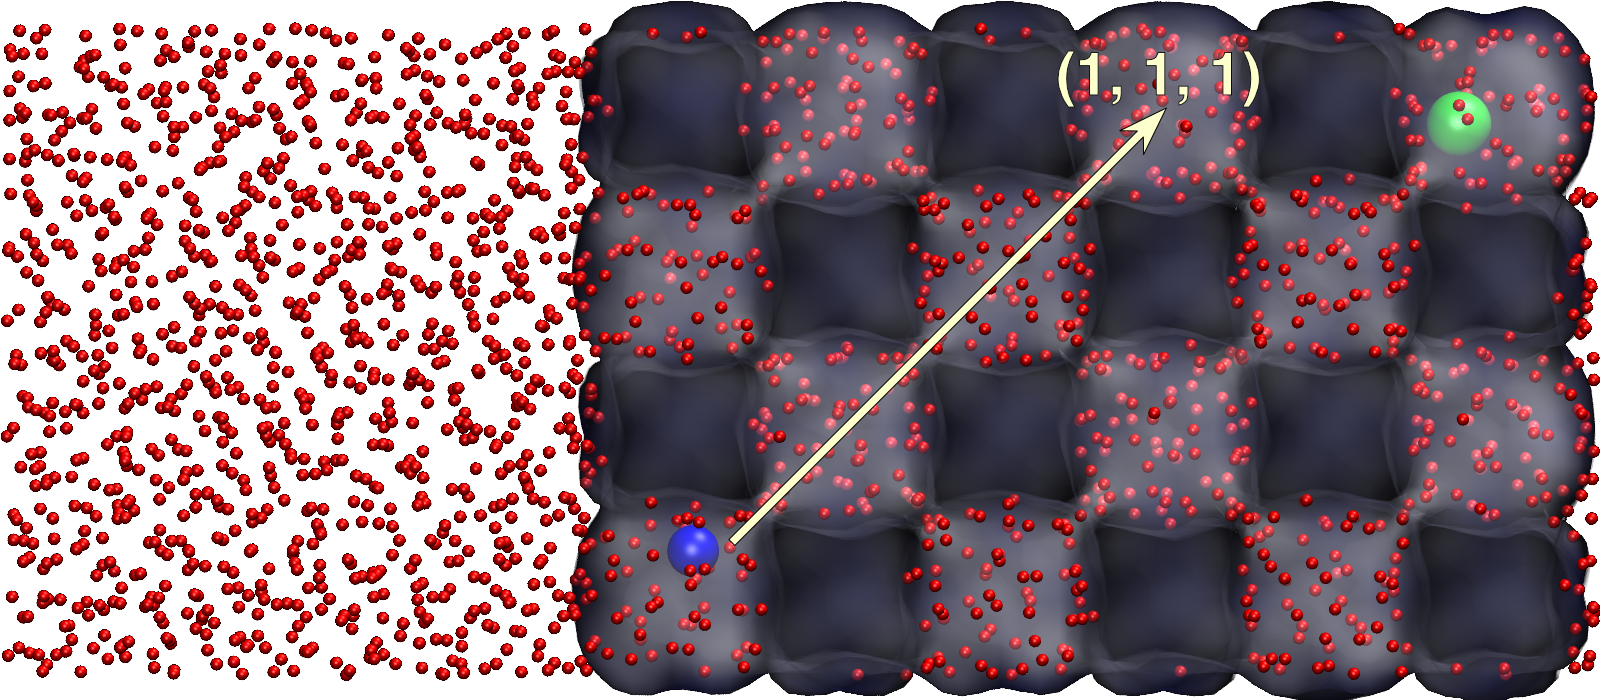
\includegraphics[width=0.9\textwidth]{figures/images/licl-zif-umbrella}
%     \caption{Representation of the system used for umbrella sampling simulation
%     to compute the free energy profile of entry of lithium ions in \ZIF8. We
%     used similar systems for the free energy profile of entry of chlorine and
%     water. Water molecules are represented in red, lithium ions in pink and
%     chlorine ion in green. \ZIF8 is represented as a transparent matrix.}
%     \label{fig:licl-zif:umbrella-system}
% \end{figure}
%
% In the previous sections, I described the behavior of intruded electrolytes in
% the pores of \ZIF8, using full periodic boundary conditions. Here, I want to
% investigate the thermodynamics of the process by which species (water molecules
% and ions) can actually enter the nanopores space, \emph{i.e.} pass through the
% windows of the material and its external surface. I have thus modeled an
% explicit water/\ZIF8 interface, depicted in
% figure~\ref{fig:licl-zif:umbrella-system}: the system here contains both water
% in the bulk state in a \SI{34}{\AA}$\times$\SI{34}{\AA}$\times$\SI{30}{\AA}
% reservoir, and water confined inside \ZIF8. I used umbrella sampling simulations
% and the WHAM analysis method\cite{WHAM} to reconstruct the free energy profile
% of a single species (\ce{Li+}, \ce{Cl-}, or \ce{H2O}) entering \ZIF8 along the
% (111) crystallographic axis. I placed the molecule of interest at \SI{5}{\AA} of
% a window between the bulk and confined water, and the corresponding counter ion
% on the other side of the \ZIF8 slab (to keep the system neutral yet minimize
% ion--ion interactions). I ran a total of 121 umbrella sampling simulation for
% each species, spaced every \SI{0.33}{\AA}. Each simulation ran for \SI{500}{ps}
% in the $NVT$ ensemble, using the last step of the previous simulation as
% starting point. The resulting free energy profile is presented in
% figure~\ref{fig:licl-zif:free}, together with the average number of neighbors at
% a given position on the axis (lower panel).
%
% \begin{figure}[ht]
%     \centering
%     % GNUPLOT: LaTeX picture with Postscript
\begingroup
  \makeatletter
  \providecommand\color[2][]{%
    \GenericError{(gnuplot) \space\space\space\@spaces}{%
      Package color not loaded in conjunction with
      terminal option `colourtext'%
    }{See the gnuplot documentation for explanation.%
    }{Either use 'blacktext' in gnuplot or load the package
      color.sty in LaTeX.}%
    \renewcommand\color[2][]{}%
  }%
  \providecommand\includegraphics[2][]{%
    \GenericError{(gnuplot) \space\space\space\@spaces}{%
      Package graphicx or graphics not loaded%
    }{See the gnuplot documentation for explanation.%
    }{The gnuplot epslatex terminal needs graphicx.sty or graphics.sty.}%
    \renewcommand\includegraphics[2][]{}%
  }%
  \providecommand\rotatebox[2]{#2}%
  \@ifundefined{ifGPcolor}{%
    \newif\ifGPcolor
    \GPcolortrue
  }{}%
  \@ifundefined{ifGPblacktext}{%
    \newif\ifGPblacktext
    \GPblacktextfalse
  }{}%
  % define a \g@addto@macro without @ in the name:
  \let\gplgaddtomacro\g@addto@macro
  % define empty templates for all commands taking text:
  \gdef\gplbacktext{}%
  \gdef\gplfronttext{}%
  \makeatother
  \ifGPblacktext
    % no textcolor at all
    \def\colorrgb#1{}%
    \def\colorgray#1{}%
  \else
    % gray or color?
    \ifGPcolor
      \def\colorrgb#1{\color[rgb]{#1}}%
      \def\colorgray#1{\color[gray]{#1}}%
      \expandafter\def\csname LTw\endcsname{\color{white}}%
      \expandafter\def\csname LTb\endcsname{\color{black}}%
      \expandafter\def\csname LTa\endcsname{\color{black}}%
      \expandafter\def\csname LT0\endcsname{\color[rgb]{1,0,0}}%
      \expandafter\def\csname LT1\endcsname{\color[rgb]{0,1,0}}%
      \expandafter\def\csname LT2\endcsname{\color[rgb]{0,0,1}}%
      \expandafter\def\csname LT3\endcsname{\color[rgb]{1,0,1}}%
      \expandafter\def\csname LT4\endcsname{\color[rgb]{0,1,1}}%
      \expandafter\def\csname LT5\endcsname{\color[rgb]{1,1,0}}%
      \expandafter\def\csname LT6\endcsname{\color[rgb]{0,0,0}}%
      \expandafter\def\csname LT7\endcsname{\color[rgb]{1,0.3,0}}%
      \expandafter\def\csname LT8\endcsname{\color[rgb]{0.5,0.5,0.5}}%
    \else
      % gray
      \def\colorrgb#1{\color{black}}%
      \def\colorgray#1{\color[gray]{#1}}%
      \expandafter\def\csname LTw\endcsname{\color{white}}%
      \expandafter\def\csname LTb\endcsname{\color{black}}%
      \expandafter\def\csname LTa\endcsname{\color{black}}%
      \expandafter\def\csname LT0\endcsname{\color{black}}%
      \expandafter\def\csname LT1\endcsname{\color{black}}%
      \expandafter\def\csname LT2\endcsname{\color{black}}%
      \expandafter\def\csname LT3\endcsname{\color{black}}%
      \expandafter\def\csname LT4\endcsname{\color{black}}%
      \expandafter\def\csname LT5\endcsname{\color{black}}%
      \expandafter\def\csname LT6\endcsname{\color{black}}%
      \expandafter\def\csname LT7\endcsname{\color{black}}%
      \expandafter\def\csname LT8\endcsname{\color{black}}%
    \fi
  \fi
    \setlength{\unitlength}{0.0500bp}%
    \ifx\gptboxheight\undefined%
      \newlength{\gptboxheight}%
      \newlength{\gptboxwidth}%
      \newsavebox{\gptboxtext}%
    \fi%
    \setlength{\fboxrule}{0.5pt}%
    \setlength{\fboxsep}{1pt}%
\begin{picture}(5660.00,5660.00)%
    \gplgaddtomacro\gplbacktext{%
      \csname LTb\endcsname%%
      \put(752,3264){\makebox(0,0)[r]{\strut{}$-10$}}%
      \csname LTb\endcsname%%
      \put(752,3627){\makebox(0,0)[r]{\strut{}$0$}}%
      \csname LTb\endcsname%%
      \put(752,3990){\makebox(0,0)[r]{\strut{}$10$}}%
      \csname LTb\endcsname%%
      \put(752,4353){\makebox(0,0)[r]{\strut{}$20$}}%
      \csname LTb\endcsname%%
      \put(752,4716){\makebox(0,0)[r]{\strut{}$30$}}%
      \csname LTb\endcsname%%
      \put(752,5079){\makebox(0,0)[r]{\strut{}$40$}}%
      \csname LTb\endcsname%%
      \put(752,5442){\makebox(0,0)[r]{\strut{}$50$}}%
      \csname LTb\endcsname%%
      \put(871,3047){\makebox(0,0){\strut{}$-20$}}%
      \csname LTb\endcsname%%
      \put(1425,3047){\makebox(0,0){\strut{}$-15$}}%
      \csname LTb\endcsname%%
      \put(1979,3047){\makebox(0,0){\strut{}$-10$}}%
      \csname LTb\endcsname%%
      \put(2533,3047){\makebox(0,0){\strut{}$-5$}}%
      \csname LTb\endcsname%%
      \put(3087,3047){\makebox(0,0){\strut{}$0$}}%
      \csname LTb\endcsname%%
      \put(3640,3047){\makebox(0,0){\strut{}$5$}}%
      \csname LTb\endcsname%%
      \put(4194,3047){\makebox(0,0){\strut{}$10$}}%
      \csname LTb\endcsname%%
      \put(4748,3047){\makebox(0,0){\strut{}$15$}}%
      \csname LTb\endcsname%%
      \put(5302,3047){\makebox(0,0){\strut{}$20$}}%
    }%
    \gplgaddtomacro\gplfronttext{%
      \csname LTb\endcsname%%
      \put(178,4353){\rotatebox{-270}{\makebox(0,0){\strut{}free energy (kcal/mol)}}}%
      \csname LTb\endcsname%%
      \put(2924,5247){\makebox(0,0)[r]{\strut{}\ce{Li}}}%
      \csname LTb\endcsname%%
      \put(2924,5030){\makebox(0,0)[r]{\strut{}\ce{Cl}}}%
      \csname LTb\endcsname%%
      \put(2924,4813){\makebox(0,0)[r]{\strut{}\ce{H2O}}}%
    }%
    \gplgaddtomacro\gplbacktext{%
      \csname LTb\endcsname%%
      \put(633,694){\makebox(0,0)[r]{\strut{}$0$}}%
      \csname LTb\endcsname%%
      \put(633,1078){\makebox(0,0)[r]{\strut{}$2$}}%
      \csname LTb\endcsname%%
      \put(633,1462){\makebox(0,0)[r]{\strut{}$4$}}%
      \csname LTb\endcsname%%
      \put(633,1845){\makebox(0,0)[r]{\strut{}$6$}}%
      \csname LTb\endcsname%%
      \put(633,2229){\makebox(0,0)[r]{\strut{}$8$}}%
      \csname LTb\endcsname%%
      \put(633,2613){\makebox(0,0)[r]{\strut{}$10$}}%
      \csname LTb\endcsname%%
      \put(752,477){\makebox(0,0){\strut{}$-20$}}%
      \csname LTb\endcsname%%
      \put(1321,477){\makebox(0,0){\strut{}$-15$}}%
      \csname LTb\endcsname%%
      \put(1890,477){\makebox(0,0){\strut{}$-10$}}%
      \csname LTb\endcsname%%
      \put(2458,477){\makebox(0,0){\strut{}$-5$}}%
      \csname LTb\endcsname%%
      \put(3027,477){\makebox(0,0){\strut{}$0$}}%
      \csname LTb\endcsname%%
      \put(3596,477){\makebox(0,0){\strut{}$5$}}%
      \csname LTb\endcsname%%
      \put(4165,477){\makebox(0,0){\strut{}$10$}}%
      \csname LTb\endcsname%%
      \put(4733,477){\makebox(0,0){\strut{}$15$}}%
      \csname LTb\endcsname%%
      \put(5302,477){\makebox(0,0){\strut{}$20$}}%
    }%
    \gplgaddtomacro\gplfronttext{%
      \csname LTb\endcsname%%
      \put(178,1653){\rotatebox{-270}{\makebox(0,0){\strut{}number of neighbors}}}%
      \csname LTb\endcsname%%
      \put(3027,152){\makebox(0,0){\strut{}x ($\AA$)}}%
    }%
    \gplbacktext
    \put(0,0){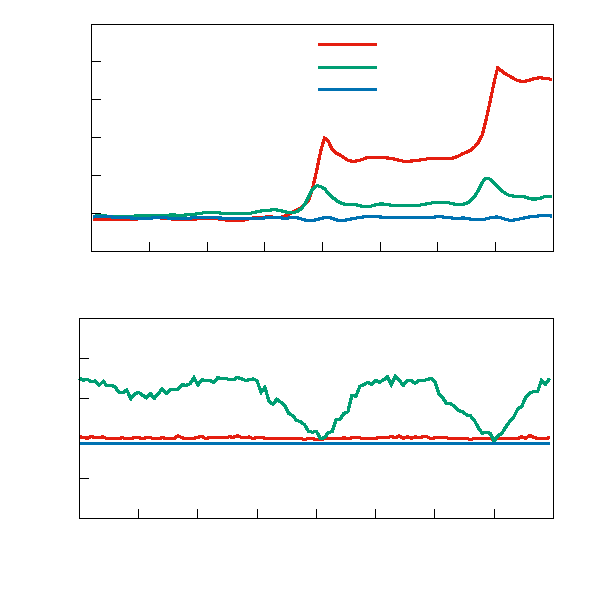
\includegraphics{licl-zif-free-energy}}%
    \gplfronttext
  \end{picture}%
\endgroup

%     \caption{Free energy profile (top) of a single molecule entering \ZIF8 and
%     corresponding number of neighbors (bottom) in the first solvation shell as
%     function of the position of the molecule along the (111) crystallographic
%     axis. The first \ZIF8 windows is at $x=0$; the $x<0$ area corresponds to
%     bulk water, and the $x>0$ area to water-filled \ZIF8. We evaluated the
%     uncertainty on the free energy profile using Monte Carlo
%     bootstrapping\cite{WHAM}, and found it to be at most \SI{0.08}{kcal/mol} for
%     \ce{H2O}, and \SI{0.3}{kcal/mol} for \ce{Cl-} and \ce{Li+}.}
%     \label{fig:licl-zif:free}
% \end{figure}
%
% The first conclusion is that there is no free energy barrier for entry of the
% water molecule: the energy profile is flat and the number of neighbors is
% constant and around 4. This is coherent with the results already presented on
% the location of water molecules inside the \ZIF8 windows and on the number of
% neighbors for water molecules inside \ZIF8. It also confirms that the nature of
% the liquid-phase intrusion process is not a kinetic limitation of water
% adsorption, but actually due to thermodynamic hydrophobicity of the framework.
% For chlorine anions, we observe two barriers on the free energy profile, which
% correspond to the \ZIF8 windows at 0 and \SI{15}{\AA}. These barriers are
% correlated to a lower number of neighbors for the anion, dropping to a value of
% 4: there is not enough space inside the window to fit a chlorine ion and 7 water
% molecules, and the anion has to partially desolvate to pass through the window
% --- explaining the presence of the free energy barrier. Outside of these
% barrier, the profile is flat and at the same level as in the bulk liquid,
% meaning that while the entry of a single chlorine ion is a rare event, at long
% thermodynamic time scale, Cl ions should be able to enter in \ZIF8. Generally
% speaking, the Cl ions have a kinetic barrier to entry in the \ZIF8.
%
% The results for Li are more surprising. We see both a high barrier at the first
% ($x=\SI{0}{\AA}$) and second ($x=\SI{15}{\AA}$) windows; and an
% energetic difference between outside and inside the pores of roughly
% \SI{15}{kcal/mol}. This energy difference is not only due to the bulk liquid to
% confined liquid transition, as it is also present in the transition between
% before and after the second window. At the same time, these barriers and energy
% differences are not linked to a difference in solvation as in the chlorine case,
% as the number of neighbors of lithium stays constant and around 4. Indeed, the
% solvation of \ce{Li+} by water is much stronger, and its solvation sphere is
% smaller in size than \ce{Cl-}. As lithium does not partially desolvate or
% rearrange to pass the barrier, the whole solvation sphere needs to go though a
% relatively small window, thus making the barrier higher. This points to a
% difference in nature between the \ce{Li+} and \ce{Cl-} ions, which will have to
% be probed further, for example by studies on other ions of different size.
%
% \newpage
% \subsection{Conclusion}
%
% Liquid intrusion of water and concentrated aqueous solutions in hydrophobic
% materials have been proposed for applications in mechanical energy storage and
% dissipation, and recently ZIF frameworks have been highlighted for the high
% energy density that they can store. However, while the process of intrusion has
% been well studied in various zeolitic materials over the last 20 years, there is
% relatively little information available on the behavior --- at the microscopic
% scale --- of water and electrolytes in hydrophobic metal--organic frameworks.
% These systems are difficult to probe experimentally, because liquid intrusion
% has to occur under high pressure. Therefore, we have used molecular dynamics
% simulations to shed some light onto the properties of LiCl aqueous solutions at
% various concentrations confined inside the pores of the \ZIF8 metal--organic
% framework. We show that the presence of the electrolyte has a moderate impact on
% the \ZIF8 framework, while the presence of the \ZIF8 matrix strongly influences
% the behavior of the confined aqueous solution, affecting the overall properties
% of the system. We also computed the free energy profile for the entry of water
% molecules and ions into the nanopores, showing a difference between anions and
% cations.
%
% While this work provides an interesting picture of the LiCl electrolytes in
% \ZIF8, it also opens a few venues for future research. The main one is the
% impact of the ion size on the properties of the confined liquid. Experiments
% have been performed experimentally with other ions of larger size, including
% KCl, and there it is not even clear what fraction of the larger cations
% (\ce{K+}) actually can diffuse inside the nanopores. Computational approaches to
% these systems will be of great help in rationalizing the experimental results
% and provide a view of the microscopic mechanisms that are behind them.
%
% Another one is to give a deeper look at the free energy barriers for ions
% passing through the windows of \ZIF8. While the windows are found, in the gas
% phase, to be very flexible and let diffuse molecules of large diameter (up to
% butane), we find that the entry of solvated species, such as ions in water, can
% be linked to a significant free energy barrier. Our free energy simulations of
% this process will have to be extended to other ions, in order to probe the
% influence of the size of both the ion and its solvation shell, but also to look
% at the influence of electrolyte concentration on the free energy profiles.
% Initial tests in this direction have shown that it should be technically
% possible, but convergence in such highly constrained systems is very difficult
% to achieve.
%
% Finally, this work focused on the \ZIF8 framework, perhaps the most archetypal
% of the ZIF materials. The influence of framework functionalization with various
% imidazolate derivatives, which has shown to greatly impact adsorption in the gas
% phase, will surely also manifest itself in the liquid-phase intrusion processes.

\newpage
\section{Adsorption of water in imogolites}

During my PhD, I worked with Laura Scalfi during her master internship in the
group to study water adsorption in the alumino-silicate nanotubes called
imogolites. This study is published in \citejournal{Scalfi2018}\cite{Scalfi2018}.

Imogolite is an alumino-silicate material, with formula \ce{Al2SiO3(OH)4}, that
was first discovered in volcanic ashes in Japan\cite{Yoshinaga1962}. It is the
only known alumino-silicate material that spontaneously forms inorganic
nanotubes, and there exists no planar equivalent material in nature --- unlike
carbon nanotubes, of which graphene is the planar form. Imogolite nanotubes are
monodisperse in diameter, and can be readily synthesized with controlled length
and diameter, for example by substituting silicon with
germanium\cite{Amara2013}. This precise control of the imogolite nanotube
dimensions is interesting for applications that rely on one-dimensional pore
channels, in fields such as nanofluidic devices, membranes for filtration and
separation, desalination, etc. Moreover, from a theoretical point of view, its
hollow cylindrical topology and tuneable size make it a very attractive model to
study the properties of fluids under confinement. Their structure was first
described by \citeauthor{Cradwick1972}\cite{Cradwick1972} from electron
diffraction measurements as a cylindrical assembly of silicon tetrahedra and
aluminum octahedra (see figure~\ref{fig:imogolite:structure}). This sheet
spontaneously folds into a nanotube because of bond length mismatch and
formation of hydrogen bonds\cite{Lee2011,Gonzalez2014}. The imogolite nanotubes
are characterized using the same nomenclature as carbon nanotubes. Both natural
and synthetic imogolite nanotubes exhibit a zigzag folding, with a variable
number $n$ of \ce{Al2O3SiOH(OH)3} units (called gibbsite units) along the
nanotube circumference. The cylindrical unit cell then contains $2n$ gibbsite
units.  Natural imogolite is a nanotube with size $n=12$, while depending on the
details of the synthesis conditions, synthetic imogolites correspond to values
of $n$ typically between 12 and 14, and sometimes larger.

\begin{figure}[b]
    \centering
    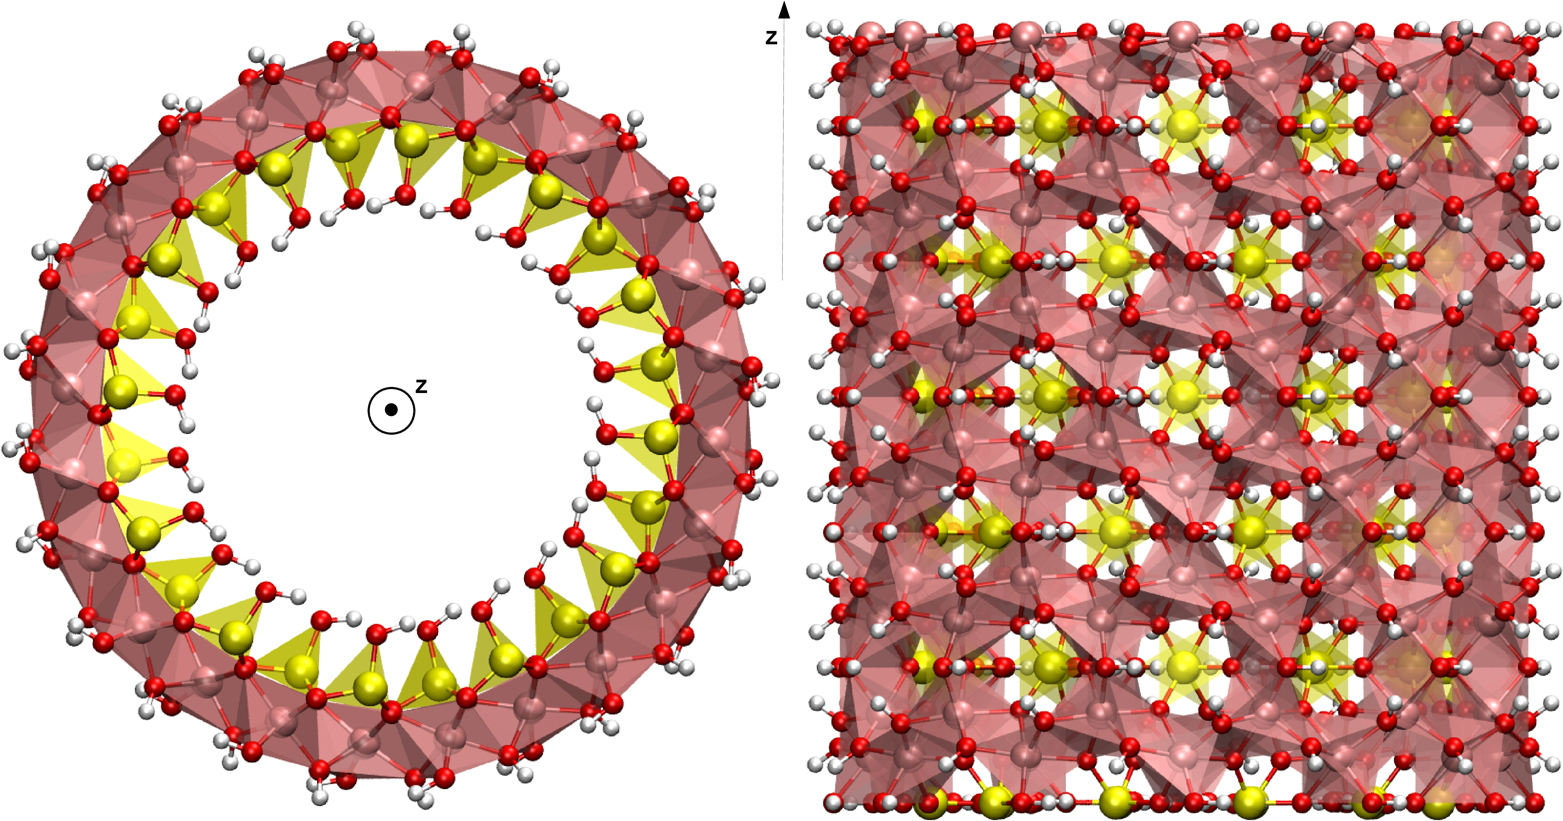
\includegraphics[width=\textwidth]{figures/images/imogolite}
    \caption{Imogolite nanotube ($n=12$) with three unit cells along the tube
    axis $z$. Color code: aluminum (pink), silicon (yellow), oxygen (red),
    hydrogen (white). Note the hydrogen bonds between silanol groups on the
    inner surface (left panel).}
    \label{fig:imogolite:structure}
\end{figure}

Although imogolites have been the subject of several experimental studies, only
a few theoretical works have been carried out until now. In particular, there is
relatively little data --- experimental or computational --- on the hydration of
these nanotubes and the behavior of the confined water molecules inside the pore
space. Imogolite nanotubes differ markedly from the more common carbon nanotubes
in both geometry and chemistry, and the behavior of water inside their pores is
still very much open. It is experimentally challenging to address these issues,
especially differentiating the water inside the nanotubes from the water
outside, and a computational approach through molecular modeling is therefore a
natural complement to the published experimental results.

A single imogolite nanotube presents two surfaces, both available for
adsorption. The outer surface is composed of a gibbsite-like sheet of aluminum
octahedra. The inner surface is formed of silicon tetrahedra with one hydroxyl
group exposed and the three other corners of the tetrahedron linked to three
aluminum octahedra. Therefore both surfaces are covered with hydroxyl groups
that are expected to have a hydrophilic behavior. Based on electrostatic
calculations, authors have suggested that the inner surface is strongly
hydrophilic whereas the outer surface might be more
hydrophobic\cite{Gustafsson2001,Guimaraes2007}. Because adsorption on the outer
surface of the nanotubes depends strongly on experimental conditions affecting
the bundling of the nanotubes, and therefore the spacing between them, we
focused on the adsorption and behavior of water confined \emph{inside} imogolite
nanotubes. Moreover, the strong curvature and limited space inside the nanotube
provide for strong confinement effects on which little experimental data is
available.

% Most of the theoretical studies on imogolite nanotubes focus on the energetics
% of empty nanotubes. The sharp monodispersity in nanotube diameters has been
% explained by both quantum chemistry and classical studies, that show the strain
% energy has a minimum for a given nanotube diameter, contrary to carbon nanotubes
% where the energetically favorable structure is that of infinite diameter (i.e.,
% the graphene slab\cite{tamura2002, guimaraes2007,
% zhao2009, demichelis2010}). Several studies also focused
% on computing vibrational spectra\cite{tamura2002,
% alvarez-ramirez2007,konduri2007} and studying the energetics
% and dynamics of the rolling of the nanotubes themselves.\cite{lee2011,
% gonzalez2014, gonzalez2016} Finally, other works have pointed
% at more complex aspects, such as defects \cite{gustafsson2001} and
% deformation or hexagonalisation of the nanotubes.\cite{tamura2002,
% Amara2014, creton2008-1}
%
% \section{Systems}
%
% \subsection{Imogolite structure}
%
% In order to produce imogolite nanotube models, we started from the structure of
% \citeauthor{Cradwick1972}\cite{Cradwick1972} for a $n=10$ nanotube
% with $C_{2n}$ symmetry. We formed a flat gibbsite-like sheet by unfolding the
% nanotube and adding hydrogen atoms (not present on the electron diffraction
% data). We relaxed the slab geometry and unit cell with density functional theory
% (DFT, see computational details in next section) in the $C_m$ space group. From
% this relaxed planar structure, we rolled back a nanotube of size $n=12$. Using
% the Bilbao Crystallographic Server\cite{Aroyo2006}, we identified the
% space groups of the nanotube to be $P4/m$. We relaxed the nanotube structure and
% cell parameters with periodic DFT calculations, with large inter-nanotube
% spacing (\SI{60}{\AA}) so that there are no interactions between nanotubes. We show
% on figure~\ref{fig::nt12-hb1}, two views from top and side of the
% $n=12$ nanotube with three unit cells along the $z$ axis.
%
% The internal surface of an imogolite nanotube can be described as a periodic
% sequence of silicon rings along the nanotube axis. Two adjacent rings are
% rotated of $\pi / n$. When dry, silanol groups within a ring form hydrogen bonds
% so that all the hydroxyl groups are in a plane normal to the nanotube axis, as
% shown in figure \ref{fig::nt12-hb1}. The internal diameter, computed between
% internal oxygens (noted \ce{O_{int}}), is \SI{12.8}{\AA} and the external diameter,
% computed between external oxygens (noted \ce{O_{ext}}), is approximately
% \SI{22}{\AA}. \citeauthor{Konduri2008}\cite{Konduri2008} highlighted that as a
% consequence the inner pore is not smooth and uniform as for the carbon nanotube,
% but the pore is rugged: narrower where there are silanol groups and larger
% between these silicon rings. One can picture the internal cavity as a hollow
% cylinder with equally spaced circular furrows in the circumference.

\subsection{Simulation methods}

\TODO: n=12

Imogolite nanotubes can have a length from \SI{10}{nm} up to a few micrometers
and experiments show that they tend to pack into bundles when dry. The periodic
pattern seems to be a monoclinic assembly \cite{Ackerman1993, Mukherjee2005}
with $\beta \approx 78${\textdegree}. Given our focus on adsorption inside the
nanotubes, following other theoretical studies, we chose to represent the
nanotubes in a hexagonal packing that is close to the monoclinic
one\cite{AlvarezRamirez2007, Konduri2008, Zang2010}. Lattice constants are
chosen to ensure close contact (but no overlap) between neighboring nanotubes,
at $a = b = \SI{24.2}{\AA}$. This choice is consistent with experiments and
other theoretical studies. Along the tube axis, we studied super-cells with
lattice parameters $c = n \times \SI{8.486}{\AA}$ where $n = 1$, 3 or 5 (where
the value of \SI{8.486}{\AA} was determined by geometry optimization with
variable cell).

% \subsection{Density Functional Theory calculations}
%
% Energy minimization of the nanotubes and slabs were performed with Density
% Functional Theory (DFT) calculations with periodic boundary conditions and the
% use of symmetry to reduce computational cost. We used these calculations with
% the CRYSTAL14\cite{dovesi2014} software package. The exchange--correlation
% functional used was the solid-adapted generalized gradient approximation (GGA)
% PBEsol, and the basis set for all atoms (Si, Al, O, H) was double-$\zeta$
% valence polarized (DZVP).
%
% We also performed DFT-based molecular dynamics simulations, aka first principles
% or \emph{ab initio} molecular dynamics (MD), as a way to generate reference data
% for comparison and validation of classical force fields. These simulations were
% run with CP2K.\cite{hutter_<span_2014} Temperature was kept constant at \SI{300}{K}
% with a CSVR (canonical sampling through velocity rescaling)
% thermostat,\cite{Bussi2007} with a time constant of \SI{200}{fs}. The timestep was
% \SI{0.5}{fs}, and the system was deuterated for computational convenience. After \SI{5}{ps}
% of equilibration, production trajectories were accumulated for \SI{30}{ps}.
%
% \subsection{Classical simulations}

Why we used classical simulations to study structure and dynamics of water in
imogolites at large timescales. We ran MD simulations in the canonical $NVT$
ensemble with the LAMMPS code\cite{Plimpton1993}, using a timestep of
\SI{0.5}{fs}. After \SI{100}{ps} of equilibration, we collected trajectories
from \SI{200}{ps} to \SI{50}{ns}, depending on the properties studied in each
case. We also performed series of Grand Canonical Monte Carlo (GCMC) simulations
with fixed chemical potential, volume and temperature $\mu VT$, to simulate the
behavior of the system on equilibrium with a reservoir at a given pressure
linked to the chemical potential. In the gas phase, water was considered to be
an ideal gas, and the chemical potential is then easily linked to the gas
pressure\cite{Desbiens2005}. Series of GCMC simulations were used to compute
adsorption isotherms, with water vapor pressure going from 2 to 3\,\SI{600}{Pa}.

To describe the interactions of the nanotube, we relied on the CLAYFF force
field\cite{Cygan2004}, which has been extensively used in the literature
\cite{Konduri2008, Zang2010, Gonzalez2016}. Water was described in the flexible
Single-Point Charge (fSPC) model\cite{Teleman1987}, which is naturally suited
for coupling with CLAYFF. CLAYFF is a general force field developed to model
clay minerals, that have the same chemical nature of the imogolite. It relies
almost exclusively on non-bonded interactions, where interatomic potentials are
the sum of electrostatic (Coulombic) and Lennard-Jones interactions. In addition
to these non-bonding interactions, CLAYFF includes a harmonic bond term for
hydroxyl bonds (\ce{O-H} stretching); and a \ce{M-O-H} harmonic bending
potential.

% \section{Results and discussion}
%
% \subsection{Validation of the force field}
%
% The CLAYFF force field has been used in the literature for classical molecular
% simulations of imogolite nanotubes,\cite{Konduri2008,
% Zang2010, gonzalez2016} owing to the similarities
% between clays and imogolite. Here, we set out to check its validity in the
% description of both neat imogolite nanotubes as well as water-filled tubes. As a
% reference, we compared it to trajectories obtained from first-principles
% molecular dynamics, where the evaluation of interatomic forces is done at the
% DFT level. We found that the structure of the nanotube itself is relatively
% rigid, and dictated by equilibrium Si---O and Al---O bond lengths, so that the
% skeleton (aluminum Al, silicon Si, and bridging oxygens O$_{\text{br}}$) is well
% reproduced with the CLAYFF potential (in both variants).
%
% \begin{figure}[ht]
% 	\centering
% 	% \includegraphics[width=0.5\linewidth]{angles}\hfill
% 	% \includegraphics[width=0.5\linewidth]{density_hint}
% 	\caption{Left: angle distributions for \ce{Si-O_{int}-H_{int}} angles (top) and \ce{Al-O_{ext}-H_{ext}} angles (bottom) for DFT (red line), CLAYFF (dark blue line) and extended-CLAYFF (sky blue line) simulations. Right: density of the internal hydrogen atoms, \ce{H_{int}}, along the nanotube axis $z$ for an empty nanotube (solid lines) and a fully hydrated nanotube (dashed lines). Data from DFT are shown in red, data from CLAYFF in dark blue, and from extended-CLAYFF in sky blue.}
%     \label{fig:imogolite:ff-angles}
% \end{figure}
%
% Secondly, we focus on the description of the inner and outer surface groups. We
% plot in figure~\ref{fig:imogolite:ff-angles} the calculated distributions of
% \ce{Si-O_{int}-H_{int}} angles for silanol groups inside the tube, and
% \ce{Al-O_{ext}-H_{ext}} angles for AlOH groups on the outer surface. There are
% clear discrepancies between CLAYFF results and reference first principles data:
% average \ce{M-O-H} angles are much larger, and their distribution broader. For
% CLAYFF, angles go all the way up to 180{\textdegree} and, for AlOH, down below
% 90{\textdegree}; this contrasts with the clearly Gaussian distributions obtained
% by DFT, and centered at 115{\textdegree} and 117{\textdegree}, for SiOH and AlOH
% respectively.
%
% In contrast, augmenting the CLAYFF force field with the additional \ce{M-O-H}
% bending term (the "extended CLAYFF") leads to a clear improvement of the
% imogolite description. The distributions of both SiOH and AlOH angles are closer
% to those obtained from first-principles MD, although the match is not perfect
% --- as could be expected for a generic force field without \emph{ad hoc}
% reparameterization. The average value of the SiOH angle with extended CLAYFF is
% 122{\textdegree}, which is 7{\textdegree} larger than the reference data. The
% same is true of the outer AlOH groups.
%
% These discrepancies in imogolite structure strongly affect water--imogolite
% interactions, and from here water adsorption, structure and dynamics. To further
% assess the necessity of using the extended CLAYFF instead of CLAYFF, we
% performed simulations of fully hydrated nanotubes, and compared them against
% data from first-principles MD. On the right panel of figure~\ref{fig:imogolite:ff-angles}, we
% show the density profiles along the nanotube axis $z$ for the internal
% hydrogens. First, we observe that in the empty nanotube, the density
% distributions are all around $z=0$ (the plane in which are located the silicon
% atoms). This allows hydrogen-bonding with other silanol groups in the same $z=0$
% plane. Secondly, upon hydration, there is a clear move of the SiOH hydrogen
% atoms toward symmetric positions at $\pm \SI{0.75}{\AA}$, due to hydrogen bonding
% with the water molecules --- a detailed analysis of this hydrated structure will
% be given below. This change in the H localization, which we observe in the
% first-principles MD, is well reproduced by the extended CLAYFF force field.
% However, it is markedly different in regular CLAYFF, where we see a unique broad
% population with two bumps. Thus the distribution of internal hydrogen atoms,
% fundamental for adsorption studies and the description of hydrated imogolites,
% is best described by the extended CLAYFF model. This aspect has been
% recently studied by \citeauthor{pouvreau2017}\cite{pouvreau2017} that similarly
% showed the necessity of a M--O--H bending term to properly describe basal and
% edge surfaces of gibbsite and brucite. From here on, we will use exclusively
% the extended CLAYFF force field.

\subsection{Water adsorption}

In order to characterize water adsorption in the gas phase and obtain
physically meaningful water uptake values, we performed GCMC simulations for
water pressure between 2 and \SI{3600}{Pa}. Full details of the simulations, done with
two different water models (SPC and TIP4P/2005) are presented in Supporting
Information, as well as isotherms. For computational reasons, rigid water models
were preferred in the GCMC calculations. We observe (figure~S1) that the
imogolite nanotube is hydrophilic, i.e. the filling occurs at a pressure below
the bulk saturation pressure. This is in agreement with the affinity of
water for silanol-rich surfaces, or zeolites with many silanol
defects\cite{Coudert2009}. The value of the pore filling pressure varies
strongly with the nature of the model chosen for the description of the water,
and the movement allowed for the silanol groups --- consistent with the findings
of \citeauthor{Zang2010}\cite{Zang2010}. We find transition pressures of
\SI{0.1}{kPa} for TIP4P05, and \SI{1}{kPa} for the SPC water model. The order of magnitude
of those values are within the range of experimental data, for example the
gravimetric study of \citeauthor{Konduri2008}\cite{Konduri2008}, which features a
smooth isotherm with water uptake in the same range (0.1 to \SI{1}{kPa}; see
figure~S1).

\begin{figure}[ht]
	\centering
	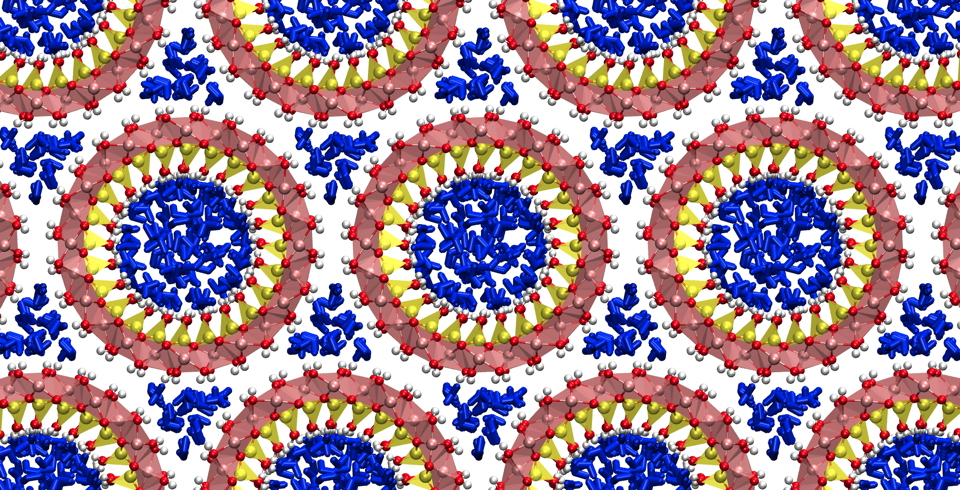
\includegraphics[width=0.8\linewidth]{figures/images/imogolite-gcmc-result}
	\caption{Fully hydrated imogolite nanotube ($n=12$) with hexagonal packing. Water molecules are represented as blue sticks.}
    \label{fig:imogolite:gcmc-result}
\end{figure}

\begin{figure}[t]
    \centering
    % GNUPLOT: LaTeX picture with Postscript
\begingroup
  \makeatletter
  \providecommand\color[2][]{%
    \GenericError{(gnuplot) \space\space\space\@spaces}{%
      Package color not loaded in conjunction with
      terminal option `colourtext'%
    }{See the gnuplot documentation for explanation.%
    }{Either use 'blacktext' in gnuplot or load the package
      color.sty in LaTeX.}%
    \renewcommand\color[2][]{}%
  }%
  \providecommand\includegraphics[2][]{%
    \GenericError{(gnuplot) \space\space\space\@spaces}{%
      Package graphicx or graphics not loaded%
    }{See the gnuplot documentation for explanation.%
    }{The gnuplot epslatex terminal needs graphicx.sty or graphics.sty.}%
    \renewcommand\includegraphics[2][]{}%
  }%
  \providecommand\rotatebox[2]{#2}%
  \@ifundefined{ifGPcolor}{%
    \newif\ifGPcolor
    \GPcolortrue
  }{}%
  \@ifundefined{ifGPblacktext}{%
    \newif\ifGPblacktext
    \GPblacktextfalse
  }{}%
  % define a \g@addto@macro without @ in the name:
  \let\gplgaddtomacro\g@addto@macro
  % define empty templates for all commands taking text:
  \gdef\gplbacktext{}%
  \gdef\gplfronttext{}%
  \makeatother
  \ifGPblacktext
    % no textcolor at all
    \def\colorrgb#1{}%
    \def\colorgray#1{}%
  \else
    % gray or color?
    \ifGPcolor
      \def\colorrgb#1{\color[rgb]{#1}}%
      \def\colorgray#1{\color[gray]{#1}}%
      \expandafter\def\csname LTw\endcsname{\color{white}}%
      \expandafter\def\csname LTb\endcsname{\color{black}}%
      \expandafter\def\csname LTa\endcsname{\color{black}}%
      \expandafter\def\csname LT0\endcsname{\color[rgb]{1,0,0}}%
      \expandafter\def\csname LT1\endcsname{\color[rgb]{0,1,0}}%
      \expandafter\def\csname LT2\endcsname{\color[rgb]{0,0,1}}%
      \expandafter\def\csname LT3\endcsname{\color[rgb]{1,0,1}}%
      \expandafter\def\csname LT4\endcsname{\color[rgb]{0,1,1}}%
      \expandafter\def\csname LT5\endcsname{\color[rgb]{1,1,0}}%
      \expandafter\def\csname LT6\endcsname{\color[rgb]{0,0,0}}%
      \expandafter\def\csname LT7\endcsname{\color[rgb]{1,0.3,0}}%
      \expandafter\def\csname LT8\endcsname{\color[rgb]{0.5,0.5,0.5}}%
    \else
      % gray
      \def\colorrgb#1{\color{black}}%
      \def\colorgray#1{\color[gray]{#1}}%
      \expandafter\def\csname LTw\endcsname{\color{white}}%
      \expandafter\def\csname LTb\endcsname{\color{black}}%
      \expandafter\def\csname LTa\endcsname{\color{black}}%
      \expandafter\def\csname LT0\endcsname{\color{black}}%
      \expandafter\def\csname LT1\endcsname{\color{black}}%
      \expandafter\def\csname LT2\endcsname{\color{black}}%
      \expandafter\def\csname LT3\endcsname{\color{black}}%
      \expandafter\def\csname LT4\endcsname{\color{black}}%
      \expandafter\def\csname LT5\endcsname{\color{black}}%
      \expandafter\def\csname LT6\endcsname{\color{black}}%
      \expandafter\def\csname LT7\endcsname{\color{black}}%
      \expandafter\def\csname LT8\endcsname{\color{black}}%
    \fi
  \fi
    \setlength{\unitlength}{0.0500bp}%
    \ifx\gptboxheight\undefined%
      \newlength{\gptboxheight}%
      \newlength{\gptboxwidth}%
      \newsavebox{\gptboxtext}%
    \fi%
    \setlength{\fboxrule}{0.5pt}%
    \setlength{\fboxsep}{1pt}%
\begin{picture}(6220.00,3400.00)%
    \gplgaddtomacro\gplbacktext{%
      \csname LTb\endcsname%%
      \put(633,694){\makebox(0,0)[r]{\strut{}$0$}}%
      \csname LTb\endcsname%%
      \put(633,1005){\makebox(0,0)[r]{\strut{}$2$}}%
      \csname LTb\endcsname%%
      \put(633,1316){\makebox(0,0)[r]{\strut{}$4$}}%
      \csname LTb\endcsname%%
      \put(633,1627){\makebox(0,0)[r]{\strut{}$6$}}%
      \csname LTb\endcsname%%
      \put(633,1938){\makebox(0,0)[r]{\strut{}$8$}}%
      \csname LTb\endcsname%%
      \put(633,2249){\makebox(0,0)[r]{\strut{}$10$}}%
      \csname LTb\endcsname%%
      \put(633,2560){\makebox(0,0)[r]{\strut{}$12$}}%
      \csname LTb\endcsname%%
      \put(633,2871){\makebox(0,0)[r]{\strut{}$14$}}%
      \csname LTb\endcsname%%
      \put(633,3182){\makebox(0,0)[r]{\strut{}$16$}}%
      \csname LTb\endcsname%%
      \put(752,477){\makebox(0,0){\strut{}$10^{-3}$}}%
      \csname LTb\endcsname%%
      \put(2029,477){\makebox(0,0){\strut{}$10^{-2}$}}%
      \csname LTb\endcsname%%
      \put(3307,477){\makebox(0,0){\strut{}$10^{-1}$}}%
      \csname LTb\endcsname%%
      \put(4585,477){\makebox(0,0){\strut{}$10^{0}$}}%
      \csname LTb\endcsname%%
      \put(5862,477){\makebox(0,0){\strut{}$10^{1}$}}%
    }%
    \gplgaddtomacro\gplfronttext{%
      \csname LTb\endcsname%%
      \put(178,1938){\rotatebox{-270}{\makebox(0,0){\strut{}water uptake (\%wt)}}}%
      \csname LTb\endcsname%%
      \put(3307,152){\makebox(0,0){\strut{}pressure (kPa)}}%
      \csname LTb\endcsname%%
      \put(2616,2966){\makebox(0,0)[r]{\strut{}\footnotesize experimental\cite{Konduri2008}}}%
      \csname LTb\endcsname%%
      \put(2616,2780){\makebox(0,0)[r]{\strut{}\footnotesize rigid nanotube\cite{Zang2010}}}%
      \csname LTb\endcsname%%
      \put(2616,2594){\makebox(0,0)[r]{\strut{}\footnotesize flexible nanotube\cite{Zang2010}}}%
      \csname LTb\endcsname%%
      \put(2616,2408){\makebox(0,0)[r]{\strut{}\footnotesize TIP4P (this work)}}%
      \csname LTb\endcsname%%
      \put(2616,2222){\makebox(0,0)[r]{\strut{}\footnotesize SPC (this work)}}%
    }%
    \gplbacktext
    \put(0,0){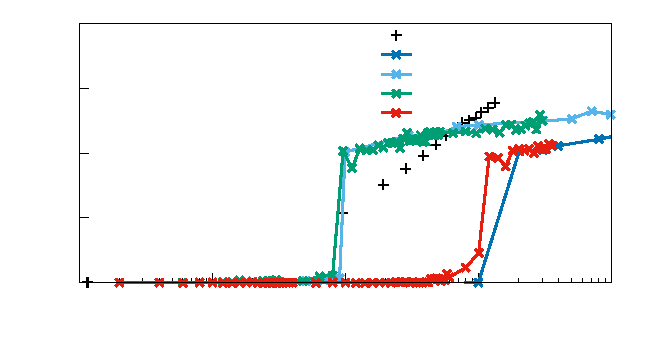
\includegraphics{imogolite-isotherms}}%
    \gplfronttext
  \end{picture}%
\endgroup

    \caption{\TODO}
    \label{fig:imogolite:isotherms}
\end{figure}

In contrast to the adsorption pressure model dependence, there is a excellent
agreement between the various models on the saturation uptake of water once the
pore is filled, i.e. on the density of the water adsorbed inside the imogolite
nanotube. Uptake is found to be 10~\% by weight after the transition, both for
the SPC and TIP4P/2005 water models. We thus derived from the GCMC calculations
an initial configuration for the simulation of the fully filled imogolite
nanotube, from the plateau of the SPC adsorption isotherm. This initial
configuration contains three nanotube ($n=12$) unit cells along the $z$ axis, 98
water molecules inside the nanotubes and 18 water molecules outside. It is
represented in figure~\ref{fig:imogolite:gcmc-result}. We used this fully
hydrated tube as a starting configuration for classical molecular dynamics
simulations, with the extended CLAYFF force field and fSPC water model.

\subsection{Structure of confined water}

\begin{figure}[t]
    \centering
    % GNUPLOT: LaTeX picture with Postscript
\begingroup
  \makeatletter
  \providecommand\color[2][]{%
    \GenericError{(gnuplot) \space\space\space\@spaces}{%
      Package color not loaded in conjunction with
      terminal option `colourtext'%
    }{See the gnuplot documentation for explanation.%
    }{Either use 'blacktext' in gnuplot or load the package
      color.sty in LaTeX.}%
    \renewcommand\color[2][]{}%
  }%
  \providecommand\includegraphics[2][]{%
    \GenericError{(gnuplot) \space\space\space\@spaces}{%
      Package graphicx or graphics not loaded%
    }{See the gnuplot documentation for explanation.%
    }{The gnuplot epslatex terminal needs graphicx.sty or graphics.sty.}%
    \renewcommand\includegraphics[2][]{}%
  }%
  \providecommand\rotatebox[2]{#2}%
  \@ifundefined{ifGPcolor}{%
    \newif\ifGPcolor
    \GPcolortrue
  }{}%
  \@ifundefined{ifGPblacktext}{%
    \newif\ifGPblacktext
    \GPblacktextfalse
  }{}%
  % define a \g@addto@macro without @ in the name:
  \let\gplgaddtomacro\g@addto@macro
  % define empty templates for all commands taking text:
  \gdef\gplbacktext{}%
  \gdef\gplfronttext{}%
  \makeatother
  \ifGPblacktext
    % no textcolor at all
    \def\colorrgb#1{}%
    \def\colorgray#1{}%
  \else
    % gray or color?
    \ifGPcolor
      \def\colorrgb#1{\color[rgb]{#1}}%
      \def\colorgray#1{\color[gray]{#1}}%
      \expandafter\def\csname LTw\endcsname{\color{white}}%
      \expandafter\def\csname LTb\endcsname{\color{black}}%
      \expandafter\def\csname LTa\endcsname{\color{black}}%
      \expandafter\def\csname LT0\endcsname{\color[rgb]{1,0,0}}%
      \expandafter\def\csname LT1\endcsname{\color[rgb]{0,1,0}}%
      \expandafter\def\csname LT2\endcsname{\color[rgb]{0,0,1}}%
      \expandafter\def\csname LT3\endcsname{\color[rgb]{1,0,1}}%
      \expandafter\def\csname LT4\endcsname{\color[rgb]{0,1,1}}%
      \expandafter\def\csname LT5\endcsname{\color[rgb]{1,1,0}}%
      \expandafter\def\csname LT6\endcsname{\color[rgb]{0,0,0}}%
      \expandafter\def\csname LT7\endcsname{\color[rgb]{1,0.3,0}}%
      \expandafter\def\csname LT8\endcsname{\color[rgb]{0.5,0.5,0.5}}%
    \else
      % gray
      \def\colorrgb#1{\color{black}}%
      \def\colorgray#1{\color[gray]{#1}}%
      \expandafter\def\csname LTw\endcsname{\color{white}}%
      \expandafter\def\csname LTb\endcsname{\color{black}}%
      \expandafter\def\csname LTa\endcsname{\color{black}}%
      \expandafter\def\csname LT0\endcsname{\color{black}}%
      \expandafter\def\csname LT1\endcsname{\color{black}}%
      \expandafter\def\csname LT2\endcsname{\color{black}}%
      \expandafter\def\csname LT3\endcsname{\color{black}}%
      \expandafter\def\csname LT4\endcsname{\color{black}}%
      \expandafter\def\csname LT5\endcsname{\color{black}}%
      \expandafter\def\csname LT6\endcsname{\color{black}}%
      \expandafter\def\csname LT7\endcsname{\color{black}}%
      \expandafter\def\csname LT8\endcsname{\color{black}}%
    \fi
  \fi
    \setlength{\unitlength}{0.0500bp}%
    \ifx\gptboxheight\undefined%
      \newlength{\gptboxheight}%
      \newlength{\gptboxwidth}%
      \newsavebox{\gptboxtext}%
    \fi%
    \setlength{\fboxrule}{0.5pt}%
    \setlength{\fboxsep}{1pt}%
\begin{picture}(7580.00,3680.00)%
    \gplgaddtomacro\gplbacktext{%
    }%
    \gplgaddtomacro\gplfronttext{%
      \csname LTb\endcsname%%
      \put(752,434){\makebox(0,0){\strut{}$-10$}}%
      \csname LTb\endcsname%%
      \put(1324,434){\makebox(0,0){\strut{}$-5$}}%
      \csname LTb\endcsname%%
      \put(1895,434){\makebox(0,0){\strut{}$0$}}%
      \csname LTb\endcsname%%
      \put(2466,434){\makebox(0,0){\strut{}$5$}}%
      \csname LTb\endcsname%%
      \put(3038,434){\makebox(0,0){\strut{}$10$}}%
      \csname LTb\endcsname%%
      \put(1895,109){\makebox(0,0){\strut{}$x\ (\AA)$}}%
      \csname LTb\endcsname%%
      \put(521,805){\makebox(0,0)[r]{\strut{}$-10$}}%
      \csname LTb\endcsname%%
      \put(521,1377){\makebox(0,0)[r]{\strut{}$-5$}}%
      \csname LTb\endcsname%%
      \put(521,1948){\makebox(0,0)[r]{\strut{}$0$}}%
      \csname LTb\endcsname%%
      \put(521,2519){\makebox(0,0)[r]{\strut{}$5$}}%
      \csname LTb\endcsname%%
      \put(521,3091){\makebox(0,0)[r]{\strut{}$10$}}%
      \csname LTb\endcsname%%
      \put(105,1948){\rotatebox{-270}{\makebox(0,0){\strut{}$y\ (\AA)$}}}%
    }%
    \gplgaddtomacro\gplbacktext{%
    }%
    \gplgaddtomacro\gplfronttext{%
      \csname LTb\endcsname%%
      \put(4542,434){\makebox(0,0){\strut{}$-10$}}%
      \csname LTb\endcsname%%
      \put(5114,434){\makebox(0,0){\strut{}$-5$}}%
      \csname LTb\endcsname%%
      \put(5685,434){\makebox(0,0){\strut{}$0$}}%
      \csname LTb\endcsname%%
      \put(6256,434){\makebox(0,0){\strut{}$5$}}%
      \csname LTb\endcsname%%
      \put(6828,434){\makebox(0,0){\strut{}$10$}}%
      \csname LTb\endcsname%%
      \put(5685,109){\makebox(0,0){\strut{}$x\ (\AA)$}}%
      \csname LTb\endcsname%%
      \put(4311,805){\makebox(0,0)[r]{\strut{}$-10$}}%
      \csname LTb\endcsname%%
      \put(4311,1377){\makebox(0,0)[r]{\strut{}$-5$}}%
      \csname LTb\endcsname%%
      \put(4311,1948){\makebox(0,0)[r]{\strut{}$0$}}%
      \csname LTb\endcsname%%
      \put(4311,2519){\makebox(0,0)[r]{\strut{}$5$}}%
      \csname LTb\endcsname%%
      \put(4311,3091){\makebox(0,0)[r]{\strut{}$10$}}%
      \csname LTb\endcsname%%
      \put(3895,1948){\rotatebox{-270}{\makebox(0,0){\strut{}$y\ (\AA)$}}}%
    }%
    \gplbacktext
    \put(0,0){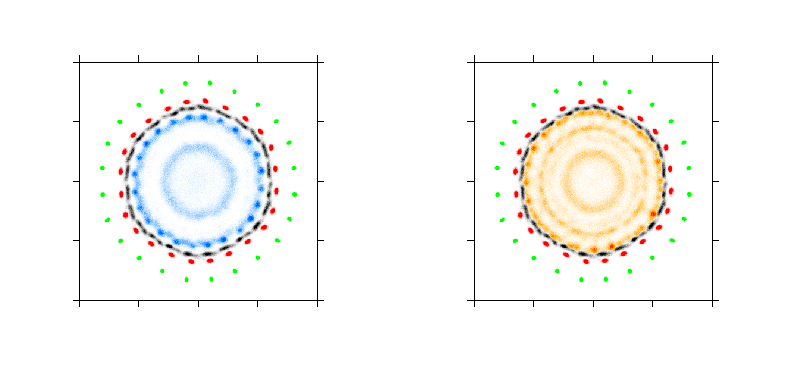
\includegraphics{imogolite-density-xy}}%
    \gplfronttext
  \end{picture}%
\endgroup

    \caption{Two-dimensional density profiles in the $xy$ plane for atoms from
    the silanols groups (Si in green, O in red, H in black) and water molecules
    (\ce{O_w} in blue on the left, \ce{H_w} in orange on the right).}
    \label{fig:imogolite:density:xy}
\end{figure}

From the analysis of the MD trajectories of the fully hydrated imogolite, we
computed density profiles of all atom types (water \ce{O_{w}} and \ce{H_{w}};
silanol groups Si, \ce{O_{int}}, and \ce{H_{int}}). They are plotted in
figure~\ref{fig:imogolite:density:xy} in the $xy$ plane, i.e. as if viewed "from the
top" of the (infinite) nanotube. From the water oxygen distribution \ce{O_w},
it is clear that there are two different populations of water molecules:
strongly structured water adsorbed next to the inner surface (a first hydration
layer, at distances between 4.5 and \SI{5.8}{\AA} from the nanotube's center), and
more disordered water filling up the center of the nanotube. This is also
clearly visible in the cylindrical distribution functions (figure \TODO), where we
see that the two populations are not completely separate, i.e. the density does
not fall to zero in-between. Furthermore, we see a slight deviation of the
nanotube from a purely circular form: the position of the Si atoms show a
slightly hexagonal deformation, due to the symmetry of the packing of nanotubes
in bundles\cite{Amara2014}. This deformation is only very
small, with Si displacements of 0.1 to \SI{0.2}{\AA} at most, due to the rigid
nature of the imogolite nanotube, especially with such a small diameter.  This
deformation is both linked to the hexagonal packing and the adsorption stress
exerted by the water molecules --- as shown previously for water/quartz
interfaces\cite{Gor2016}, and more generally for adsorbates in soft porous
materials\cite{Neimark2009, Mouhat2015}. In the case of imogolite, the stress
exerted is counterbalanced by the relative stiffness of the nanotube, although
the extent and details of the deformation depend on the packing of the
nanotubes. For example\citeauthor{Creton2008}\cite{Creton2008}, used a
larger distance between the nanotubes and observed a transition between an
ellipsoid shape to a more cylindrical shape when increasing water densities.

\begin{figure}[t]
    \centering
    % GNUPLOT: LaTeX picture with Postscript
\begingroup
  \makeatletter
  \providecommand\color[2][]{%
    \GenericError{(gnuplot) \space\space\space\@spaces}{%
      Package color not loaded in conjunction with
      terminal option `colourtext'%
    }{See the gnuplot documentation for explanation.%
    }{Either use 'blacktext' in gnuplot or load the package
      color.sty in LaTeX.}%
    \renewcommand\color[2][]{}%
  }%
  \providecommand\includegraphics[2][]{%
    \GenericError{(gnuplot) \space\space\space\@spaces}{%
      Package graphicx or graphics not loaded%
    }{See the gnuplot documentation for explanation.%
    }{The gnuplot epslatex terminal needs graphicx.sty or graphics.sty.}%
    \renewcommand\includegraphics[2][]{}%
  }%
  \providecommand\rotatebox[2]{#2}%
  \@ifundefined{ifGPcolor}{%
    \newif\ifGPcolor
    \GPcolortrue
  }{}%
  \@ifundefined{ifGPblacktext}{%
    \newif\ifGPblacktext
    \GPblacktextfalse
  }{}%
  % define a \g@addto@macro without @ in the name:
  \let\gplgaddtomacro\g@addto@macro
  % define empty templates for all commands taking text:
  \gdef\gplbacktext{}%
  \gdef\gplfronttext{}%
  \makeatother
  \ifGPblacktext
    % no textcolor at all
    \def\colorrgb#1{}%
    \def\colorgray#1{}%
  \else
    % gray or color?
    \ifGPcolor
      \def\colorrgb#1{\color[rgb]{#1}}%
      \def\colorgray#1{\color[gray]{#1}}%
      \expandafter\def\csname LTw\endcsname{\color{white}}%
      \expandafter\def\csname LTb\endcsname{\color{black}}%
      \expandafter\def\csname LTa\endcsname{\color{black}}%
      \expandafter\def\csname LT0\endcsname{\color[rgb]{1,0,0}}%
      \expandafter\def\csname LT1\endcsname{\color[rgb]{0,1,0}}%
      \expandafter\def\csname LT2\endcsname{\color[rgb]{0,0,1}}%
      \expandafter\def\csname LT3\endcsname{\color[rgb]{1,0,1}}%
      \expandafter\def\csname LT4\endcsname{\color[rgb]{0,1,1}}%
      \expandafter\def\csname LT5\endcsname{\color[rgb]{1,1,0}}%
      \expandafter\def\csname LT6\endcsname{\color[rgb]{0,0,0}}%
      \expandafter\def\csname LT7\endcsname{\color[rgb]{1,0.3,0}}%
      \expandafter\def\csname LT8\endcsname{\color[rgb]{0.5,0.5,0.5}}%
    \else
      % gray
      \def\colorrgb#1{\color{black}}%
      \def\colorgray#1{\color[gray]{#1}}%
      \expandafter\def\csname LTw\endcsname{\color{white}}%
      \expandafter\def\csname LTb\endcsname{\color{black}}%
      \expandafter\def\csname LTa\endcsname{\color{black}}%
      \expandafter\def\csname LT0\endcsname{\color{black}}%
      \expandafter\def\csname LT1\endcsname{\color{black}}%
      \expandafter\def\csname LT2\endcsname{\color{black}}%
      \expandafter\def\csname LT3\endcsname{\color{black}}%
      \expandafter\def\csname LT4\endcsname{\color{black}}%
      \expandafter\def\csname LT5\endcsname{\color{black}}%
      \expandafter\def\csname LT6\endcsname{\color{black}}%
      \expandafter\def\csname LT7\endcsname{\color{black}}%
      \expandafter\def\csname LT8\endcsname{\color{black}}%
    \fi
  \fi
    \setlength{\unitlength}{0.0500bp}%
    \ifx\gptboxheight\undefined%
      \newlength{\gptboxheight}%
      \newlength{\gptboxwidth}%
      \newsavebox{\gptboxtext}%
    \fi%
    \setlength{\fboxrule}{0.5pt}%
    \setlength{\fboxsep}{1pt}%
\begin{picture}(5660.00,4520.00)%
    \gplgaddtomacro\gplbacktext{%
    }%
    \gplgaddtomacro\gplfronttext{%
      \csname LTb\endcsname%%
      \put(712,2212){\makebox(0,0){\strut{}$-10$}}%
      \csname LTb\endcsname%%
      \put(1750,2212){\makebox(0,0){\strut{}$-5$}}%
      \csname LTb\endcsname%%
      \put(2787,2212){\makebox(0,0){\strut{}$0$}}%
      \csname LTb\endcsname%%
      \put(3824,2212){\makebox(0,0){\strut{}$5$}}%
      \csname LTb\endcsname%%
      \put(4862,2212){\makebox(0,0){\strut{}$10$}}%
      \csname LTb\endcsname%%
      \put(575,2440){\makebox(0,0)[r]{\strut{}$0$}}%
      \csname LTb\endcsname%%
      \put(575,2755){\makebox(0,0)[r]{\strut{}$2$}}%
      \csname LTb\endcsname%%
      \put(575,3069){\makebox(0,0)[r]{\strut{}$4$}}%
      \csname LTb\endcsname%%
      \put(575,3383){\makebox(0,0)[r]{\strut{}$6$}}%
      \csname LTb\endcsname%%
      \put(575,3697){\makebox(0,0)[r]{\strut{}$8$}}%
      \csname LTb\endcsname%%
      \put(575,4012){\makebox(0,0)[r]{\strut{}$10$}}%
      \csname LTb\endcsname%%
      \put(278,3226){\rotatebox{-270}{\makebox(0,0){\strut{}$r\ (\AA)$}}}%
    }%
    \gplgaddtomacro\gplbacktext{%
    }%
    \gplgaddtomacro\gplfronttext{%
      \csname LTb\endcsname%%
      \put(712,373){\makebox(0,0){\strut{}$-10$}}%
      \csname LTb\endcsname%%
      \put(1750,373){\makebox(0,0){\strut{}$-5$}}%
      \csname LTb\endcsname%%
      \put(2787,373){\makebox(0,0){\strut{}$0$}}%
      \csname LTb\endcsname%%
      \put(3824,373){\makebox(0,0){\strut{}$5$}}%
      \csname LTb\endcsname%%
      \put(4862,373){\makebox(0,0){\strut{}$10$}}%
      \csname LTb\endcsname%%
      \put(2787,48){\makebox(0,0){\strut{}$z\ (\AA)$}}%
      \csname LTb\endcsname%%
      \put(524,574){\makebox(0,0)[r]{\strut{}$0$}}%
      \csname LTb\endcsname%%
      \put(524,818){\makebox(0,0)[r]{\strut{}$2$}}%
      \csname LTb\endcsname%%
      \put(524,1062){\makebox(0,0)[r]{\strut{}$4$}}%
      \csname LTb\endcsname%%
      \put(524,1304){\makebox(0,0)[r]{\strut{}$6$}}%
      \csname LTb\endcsname%%
      \put(524,1548){\makebox(0,0)[r]{\strut{}$8$}}%
      \csname LTb\endcsname%%
      \put(524,1792){\makebox(0,0)[r]{\strut{}$10$}}%
      \csname LTb\endcsname%%
      \put(227,1183){\rotatebox{-270}{\makebox(0,0){\strut{}$r\ (\AA)$}}}%
    }%
    \gplbacktext
    \put(0,0){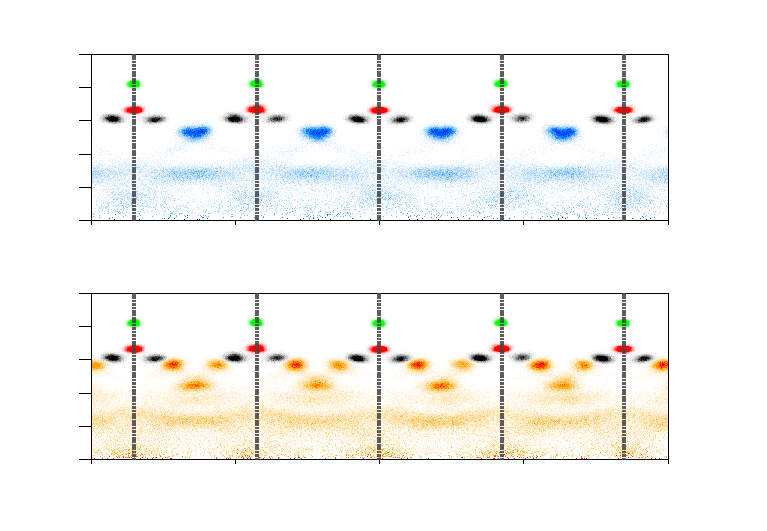
\includegraphics{imogolite-density-rz}}%
    \gplfronttext
  \end{picture}%
\endgroup

    \caption{Two-dimensional density profiles (the radial dimension versus the
    projection along the $z$ axis) for surface atoms (Si, O, H) and water atoms
    (\ce{O_w}, \ce{H_w}). Silicon rings are indicated by dashed lines.}
    \label{fig:imogolite:density:rz}
\end{figure}

To better understand the structuration of the first adsorbed layer, we plot in
figure~\ref{fig:imogolite:density:rz} the same densities, but this time as a function of
cylindrical coordinates $z$ and $\rho$, where $\rho$ is the distance to the
central axis of the nanotube. There, the strongly preferential location for the
confined water oxygen atoms becomes clear: the water molecules sit in the wider
furrows, situated in-between two rings of silanol groups (SiOH rings are
located every \SI{4.25}{\AA} along the $z$ axis, and are depicted on
figure~\ref{fig:imogolite:density:rz} by dotted lines). This preferential
localization of the adsorbed water contrasts sharply with that of water inside
carbon nanotubes, whose internal surface is smoother. It was, however,
demonstrated in other nanopores of small dimensions with "dangling" hydroxyl
groups accessible to the water for hydrogen-bonding\cite{Haigis2013}.

These molecules are strongly hydrogen-bonded to the silanol groups, as indicated
by the well-defined positions for \ce{H_{int}} atoms, which are rearranged
compared to their relaxed position. Indeed, in the dry imogolite nanotube, the
most stable position for the internal hydrogen atoms is in the silanol ring
plane ($z = 0$), where they are pointing toward a neighboring \ce{O_{int}} atom.
This conformation allows the formation a relatively weak hydrogen bond, because
the \ce{O_{int}-H_{int}$\cdots$O_{int}} distance is large. In the hydrated tube,
the hydrogen atoms' most common position is shifted out of that silanol ring
plane (see figure~\ref{fig:imogolite:density:rz}). This is reflected by a change in the
\ce{O_{br}-Si-O_{int}-H_{int}} dihedral angle (see figure~S3), which goes from
0{\textdegree} to 60{\textdegree}; where \ce{O_{br}} is the oxygen atom bridging
the aluminum to the silicon.

We thus propose the following model to better visualize and understand the
structure of the adsorbed water. We model the inner surface of the nanotube as a
periodic sequence of triangles, where each silanol group SiOH is a vertex. The
Si--Si and O--O radial distribution functions show two first neighbor peaks at
4.2 and \SI{4.7}{\AA} for silicon, and at 3.3 and \SI{4.6}{\AA} for internal oxygens.
This means that the triangles are isosceles with two angles of 66.5{\textdegree}
and one angle of 47{\textdegree}. This pattern is depicted on
figure~\ref{fig:imogolite:hbonds:sites}. Above the center of each triangle is a potential water
adsorption site. However, analysis of the sites show that no neighboring sites
in the same $xy$ plane can be occupied at the same time, due to short-distance
intermolecular repulsion of water molecules, so that at most half of the
adsorption sites are occupied in the filled tube. Then, each of the hydrogen
atoms of the SiOH groups that form the vertices of a triangle will point toward
one of the three occupied neighboring adsorption sites.

\begin{figure}[t]
	\centering
	% \includegraphics[width=0.7\linewidth]{model}
	\caption{Illustration of the model on the $n=12$ nanotube (only half of the nanotube is shown). The triangular adsorption sites are highlighted by drawing yellow triangles between silicon atoms and red triangles between oxygen atoms. In the right panel, water molecules within the first adsorption layer are drawn and hydrogen bonds are depicted in dotted blue sticks.}
    \label{fig:imogolite:hbonds:sites}
\end{figure}

\begin{figure}[t]
  \centering
  % \includegraphics[width=.8\linewidth]{density_flat}
  % \includegraphics[width=.8\linewidth]{density_flat_hw}
  % \includegraphics[width=.8\linewidth]{density_flat_hint}
  \caption{Density profiles on the flattened hydrated nanotube planes for water oxygen, water hydrogen and internal hydrogen. The circular coordinate corresponds to a curvilinear abscissa that draws a circle of radius $R = 6.5$ {\AA} centered on the axis $z$. On all the graphs, internal oxygens appear as yellow dots.}
  \label{fig:imogolite:density:circular}
\end{figure}

A final visualization can be obtained by a density plot of O and H atoms, where
the density is mapped against $z$ and a circular coordinate, as if a slice of
the nanotube had been "cut and unrolled". These densities are presented in
figure~\ref{fig:imogolite:density:circular}. Red dotted lines show the SiOH rings, while orange
dotted lines show the triangular mesh described above. The adsorption sites on
top of each triangle are clearly visible. We further see that there is a strong
anisotropy of the system, where there is possible circular movement of the water
molecules in-between sites in the same $z$ plane, while there is no observed
density crossing the silanol rings, as already observed by
\citeauthor{Creton2008}\cite{Creton2008}. This shows that there is surface
diffusion of water molecules, but only in the $xy$ plane.

\subsection{Hydrogen bonding patterns}

The localization of the first layer of adsorbed water on the inner surface of
the imogolite nanotube, and the strong hydrogen bonds that are created with the
tube's silanol groups, make the first layer of water strongly ordered. We can
see on figure~\ref{fig:imogolite:density:rz} (bottom panel) that this includes rotational
ordering of the water molecules, with three marked preferential positions for
their hydrogen atoms at room temperature. Two of those, equivalent by symmetry,
correspond to the formation of a hydrogen bond, donated by the water molecule to
the silanol group (acting as acceptor). The third position corresponds to a
hydrogen atom "dangling" toward the inside of the nanotube. Because the water
molecules have 2 hydrogen atoms that can occupy these positions, there are 3
possible geometries, summarized on figure~\ref{fig:imogolite:hbonds:surface}: a water molecule
can be donating two hydrogen bonds (case A); accepting one and donating one
(case B); or accepting two hydrogen bonds from neighboring silanol groups (case
C).

\begin{figure}
\centering
% \includegraphics[width=0.5\linewidth]{waters}
	\caption{Three possible geometries of water adsorbed in the first layer of the imogolite inner surface.}
    \label{fig:imogolite:hbonds:surface}
\end{figure}


% In this section, we quantified the hydrogen-bond network and dynamics with a set
% of geometric criteria, that are commonly used in the literature for hydrogen
% bonds in water. We consider a hydrogen bond {D---H$\cdots$A} to be present
% between donor atom D and acceptor atom A if, and only if, the D$\cdots$A
% distance is less than \SI{3.5}{\AA} and the $\widehat{\text{HDA}}$ angle is less
% than 30{\textdegree}.\cite{Luzar_hydrogen-bond_1996} We performed hydrogen bond
% analysis on the hydrated and empty nanotubes, and differentiated the types of
% hydrogen bonds according to the donor and acceptor groups. Water hydroxyls and
% silanols can both be donor and acceptor.


The average number of hydrogen bonds formed during the trajectory is presented
in table~\ref{tab:imogolite:hbonds:count}. The change in silanol--silanol hydrogen bonding
confirms the structural change upon adsorption: when the nanotube is empty,
approximately half of the silanol groups are linked by a hydrogen bond within
silicon rings (as detected per our rather strict criteria). When hydrated, only
2\% form a hydrogen bond with another silanol group. Regarding the hydrogen
bonds between a water molecule and the surface, 94\% of the silanol groups
donate a hydrogen bond to a water molecule and each silanol group receives on
average 0.96 hydrogen bonds from water. Since a silanol group can donate only 1
hydrogen bond and can receive 1 or 2 hydrogen bonds, the bonding possibilities
of the surface are extensively used. Within the nanotube, on average 57\% of
water molecules receive or donate at least one hydrogen bond from or to a
silanol group, i.e. are in the first adsorbed layer.


\begin{table}[t]
\centering
\begin{tabular}{|c|c|c|c|}
\hline
Donor   & Acceptor & Empty Nanotube  & Hydrated Nanotube \\ \hline
Silanol & Silanol  & $35.4 \pm 2.3$  & $2.0  \pm 1.3$    \\ \hline
Water   & Silanol  &                 & $69.0 \pm 2.1$    \\ \hline
Silanol & Water    &                 & $68.7 \pm 1.7$    \\ \hline
Water   & Water    &                 & $112.4 \pm 3.7$   \\ \hline
\end{tabular}
\caption{Average number of hydrogen bonds ($\pm$ the standard deviation) for given donor-acceptor pairs along a 1 ns trajectory of empty and hydrated nanotubes. Total number of silanol groups: 72; total number of water molecules: 98.}
\label{tab:imogolite:hbonds:count}
\end{table}

\begin{table}[t]
\centering
\begin{tabular}{|c|c|c|c|c|c|}
\hline
Pattern & Occurrence & Donating & Accepting & Donating & Accepting\\
 & & to silanol & from silanol & to water & from water \\ \hline
1 & 22.4\% & 0 & 0 & 2 & 2 \\ \hline
2 & 14.9\% & 1 & 2 & 1 & 0 \\ \hline
3 & 9.3\% & 2 & 1 & 0 & 1 \\ \hline
4 & 7.8\% & 0 & 0 & 2 & 1 \\ \hline
5 & 7.3\% & 1 & 1 & 1 & 1 \\ \hline
6 & 6.3\% & 1 & 1 & 1 & 0 \\ \hline
\end{tabular}
\caption{Occurrence of the most recurrent patterns of hydrogen bonding characterized by the number of bonds given to silanol and water and received from silanol and water. Percentages are given with respect to the total number of water molecules.}
\label{tab:imogolite:hbonds:patterns}
\end{table}


To further characterize the local hydrogen bond network, we considered all 4
singular hydrogen bonding behaviors possible for a single water molecule:
donating to a silanol or a water molecule, or accepting from either. Each of
these singular behaviors can appear zero, once, or twice. The patterns that
represent more than {5\%} of the occurences found over the whole trajectory are
described in table~\ref{tab:imogolite:hbonds:patterns}.


\begin{figure}[t]
  % \includegraphics[width=\linewidth]{HB3}
  % \includegraphics[width=\linewidth]{HB5}
  % \includegraphics[width=\linewidth]{HB61}
\caption{Illustration of the most common hydrogen bonding patterns for water in an imogolite nanotube. For the numbering of patterns, see table~\ref{tab:imogolite:hbonds:patterns}.}
\label{fig:imogolite:hbonds:patterns}
\end{figure}


The six patterns highlighted by this analysis can be divided in two groups: (i)
water molecules that do not form any hydrogen bond with a silanol group
(patterns 1 and 4), that can have either 4 hydrogen bonds (tetragonal
arrangement) or 3 H bonds, similarly to bulk water; and (ii) molecules whose
adsorption on the inner surface of the nanotube involves at least one hydrogen
bond (types 2, 3, 5 and 6). It is worth noting that the mean number of hydrogen
bonds for a water molecule not bonded to the surface is 3.65, slightly higher
than the bulk value for fSPC water (3.60 hydroben bonds per water molecule). The
most common patterns are represented in
figure~\ref{fig:imogolite:hbonds:patterns}. For adsorbed molecules, the most
common pattern is an "upright" water molecule (pattern 2), in a plane bisecting
the triangular adsorption site.  This water molecule receives two H bonds from
two silanol groups and donates one hydrogen bond to the third silanol. A water
hydroxyl group is left pointing toward the center of the nanotube, free to
donate a hydrogen bond to a water molecule of the second layer. This creates a
structuration of the adsorbed water beyond the first layer, which is clearly
visible in the density maps (figures~\ref{fig:imogolite:density:xy} and
\ref{fig:imogolite:density:rz}), with a favorable position for water oxygen
atoms across that pending hydroxyl group. It also defines an equilibrium
distance between the first and second layer of adsorption, which corresponds to
a water--water hydrogen bond length.

The second most common pattern for the first layer of water is a water molecule
lying "flat" on the inner imogolite surface, donating two H bonds to
neighboring silanol groups and receiving one from the third silanol neighbor.
This allows the formation of a fourth hydrogen bond from a water molecule
outside of the first layer. In this case the direction of the hydrogen bond is
less constrained, explaining the "diffuse" part of the oxygen density in the
second water layer, seen in figure~\ref{fig:imogolite:density:rz}.

The large possibilities of organization of the first layer of adsorbed water
molecules, with orientational disorder, is reminiscent of the theory of
\citeauthor{Bernal1933}\cite{Bernal1933} regarding ice rules. From the
energetics of each individual configurations, as well as the frustration arising
from constraints (no more than two H bonds can be donated or received, and no
two neighboring adsorption sites can be populated at the same time), we believe
that a model of the orientational disorder in that strongly bound layer of
adsorbed water could be constructed, possibly explaining why the adsorption
sites are only occupied at nearly {38\%} at saturation uptake.

\subsection{Water dynamics}

From the structural analysis of the water density and the hydrogen bonds in the
adsorbed water, there are clear hints at the dynamic nature of the system and
the lability of the water molecules. We have seen that hydrogen bond patterns
are statistically distributed among several configurations, and that there is
anisotropic surface diffusion in the first layer of adsorbed water (see
figure~\ref{fig:imogolite:density:circular} and accompanying text). Analysis of trajectories shows
that this surface diffusion occurs without breaking all the hydrogen bonds
involved. By breaking a single hydrogen bond, an adsorbed water molecule can
flip around the axis formed by the remaining silanol groups, and thereby
diffuses to the adjacent site, then reforms a hydrogen bond with
another SiOH group. Since the triangular sites are isosceles and the surface is
curved, the flip is easier and requires less configurational change within the
furrows, than crossing the silicon rings. This explains the preferential
circular diffusion as opposed to the axial diffusion in fully loaded nanotube.
In this section, we go further to quantify the dynamics of the water inside the
imogolite nanotube.

To do so, we calculated autocorrelation functions of the presence of water
molecules, both within the first adsorption layer and in the less-ordered "core"
of the tube. Due to the relatively slow dynamics of the strongly-confined water,
these quantities were calculated from \SI{50}{ns} classical trajectories. For
all three possible donor--acceptor hydrogen bond types, we computed
autocorrelation functions. From these autocorrelation functions, the lifetime of
each H bond type was extracted, and are presented in
table~\ref{tab:imogolite:hbonds:lifetime}. The autocorrelation decay is not
strictly exponential, because the hydrogen bonds form multiple populations
(first and second layer, etc.) with different decays.


\begin{figure}[t]
    \centering
    % \includegraphics[width=\linewidth]{HBlifetime}
    % \includegraphics[width=\linewidth]{lifetime}
    \caption{(a) Autocorrelation of the hydrogen bond existence for three types of donor-acceptor couples: water-silanol (black line), silanol-water (blue line) and water-water (red line).\\ (b) Autocorrelation of presence in the first adsorbed layer. The computed data (black line) was fitted by an exponential function (red line), $y = 1 + 0.42 (\exp(-\frac{x}{0.41})-1)$.}
    \label{fig:imogolite:hbonds:lifetime}
\end{figure}

\begin{table}[t]
\centering
\begin{tabular}{|c|c|c|c|c|c|}
\hline
Donor & Acceptor & Characteristic time $\tau$ \\
\hline
Water & Water & 4.43 ps \\
\hline
Water & Silanol & 57.43 ps\\
\hline
Silanol & Water & 123.5 ps \\
\hline
\end{tabular}
\caption{Characteristic lifetime for hydrogen bonds calculated from the time length for the autocorrelation function to decay to 50\%.}
\label{tab:imogolite:hbonds:lifetime}
\end{table}


First, looking at the water--water hydrogen bonds, we see that their lifetime is
roughly 2 times higher in the imogolite nanotube than in bulk water (calculated
at \SI{2.67}{ps} from a simulation of pure fSPC water). This slow down of the water
dynamics under confinement has been well studied and explained in previous work,
and is due in part to the stronger organization of the water, and in part to
excluded volume effects (a water molecule finding fewer partners to "switch" a
hydrogen bond to)\cite{Fogarty2014, Fogarty2014-2}. Secondly, we
see that hydrogen bonds between water and the silanol-rich surface have a
lifetime more than an order of magnitude greater than water--water H bonds. A
study on hydrogen bonding of water on the $\alpha$-quartz interface --- whose
(001) surface is chemically similar to imogolite, in that it presents geminal
silanol groups --- calculated persistence times of SiOH--water hydrogen bonds
between 160 and \SI{170}{fs}\cite{Ozkanlar2013}. The extremely large
difference, and the very strong bonding of water on the imogolite inner surface,
can be explained by the cooperative effect of the formation of three hydrogen
bonds, on top of which is present the generic confinement slow-down.

We also investigated the residence time of water molecules in the first adsorbed
layer, inside the imogolite nanotube. There are two ways to define the "first
layer", by using geometrical radius, or by considering molecules that form at
least one hydrogen bond with the surface. We chose the latter option, which is
more chemically robust. The time autocorrelation function deriving from it is
plotted in figure~\ref{fig:imogolite:hbonds:lifetime}. It shows an exponential decay, and
reaches a plateau at 57\%, i.e. the average percentage of water molecules that
belong to that first layer. The decay time for the autocorrelation function is
found to be \SI{410}{ps}. This is two or four times larger than the indicative
lifetimes of hydrogen bonds with the surface (donated or received by the silanol
group, respectively). This confirms the existence of an "inner surface
diffusion" mechanism that allows diffusion between adsorption sites without
exiting the layer itself. We can also compare this lifetime to residence times
in protein adsorption sites. For example, for myoglobin\cite{Makarov2000},
residence times span from 10 to \SI{450}{ps} where the unusually high residence
times ($> \SI{80}{ps}$) correspond to water trapped either in the cavities
inside the protein or in the grooves and concave regions.

To complete this study, we extracted diffusion coefficients from mean square
displacement (figure \TODO) of water molecules in the nanotube. We find a diffusion
coefficient in the $z$ axis of $\SI{3.5e-6}{cm^2/s}$, which is three times
smaller than the coefficient calculated by \citeauthor{Zang2009}\cite{Zang2009}
for a similar but lower water density. Moreover, we do not see a long-time
diffusive behavior in the $xy$ plane because of the confinement.

\subsection{Conclusions}

This study of the properties of water adsorbed inside hydrophilic imogolite
nanotubes was motivated by the understanding of the specific behavior of water
due to its tight confinement, with numerous silanol groups on the inner surface
of the nanotubes. Because the strong interactions between water and imogolite,
and the slow dynamics of the confined water, we relied on a classical force
field in order to perform molecular dynamics studies. We validated the CLAYFF
force field, and found that it had to be employed in its extended version ---
with a Si--O--H bending term --- in order to correctly reproduce the reference
data we had produced from first-principles molecular dynamics. This is in
contrast with conventional clay materials, where this term is not as important,
and is ascribed to the strong curvature of the imogolite surface.

We then developed a model for the structure of adsorbed water, based on the
calculated atomic densities and statistical analysis of the hydrogen bonding
patterns observed between water molecules and silanol groups. We show that
adsorption in the first layer vicinal to the imogolite tube can be described by
an anisotropic triangular lattice of adsorption sites, which are not fully
populated. We showed that interactions between the water molecules adsorbed at
neighboring sites are complex, based on (i) exclusion of some nearest neighbor
pairs (where the sites are too close to be occupied at the same time), and (ii)
the number of hydrogen bonds donated (and accepted) by the water molecules to
(and from) neighboring silanol groups. Maximizing the number of hydrogen bonds
created, while adhering to these rules, creates frustration in the system and
leads to the emergence of a heavily disordered state. This situation is very
similar to the Bernal--Fowler rules describing the orientation of water
molecules in ice\cite{Bernal1933}. Finally, we also characterized the
dynamics of the confined water molecules, as well as the hydrogen bonds. We find
that in addition to the generic effect of slow-down of confined water, the
strong interactions of water molecules with the silanol groups giving rise to
lifetimes that compare to typical residence times of water in protein adsorption
sites.

In the future, it would be interesting to extend this study of the structure of
adsorbed water at varying temperature, or with changes in the imogolite nanotube
size (from the value of $n=12$ repeating units used in this study). Another
noteworthy perspective would be to consider the possibility of partial or total
functionalization of the silanol groups --- replacing for example some of the
hydrophilic --SiOH groups with hydrophobic --SiOCH$_{\text{3}}$. This would
affect the overall affinity of the internal surface of the imogolite nanotubes
for water, tuning them from very hydrophilic to potentially
hydrophobic\cite{Bonelli2016}, and changing the thermodynamics of adsorption. It
would also introduce more frustration into the adsorbed water and change the
"ice rules", affecting the structure of the confined phase. This could be
studied by atomistic simulations, as was done here, or at a more fundamental
scale by an Ising-type model of the adsorbed water molecules, dictated by the
energies of the various possible configurations of neighbording water molecules
and silanol groups.

\OnlyInSubfile{\printbibliography}

\end{document}
